\documentclass[12pt,a4paper]{memoir}
% custom commands
\newcommand{\version}[1]{\def\theversion{#1}}
\newcommand{\subtitle}[1]{\def\thesubtitle{#1}}

\newcommand{\authors}[1]{\def\theauthors{#1}\author{#1}}
\newcommand{\supervisor}[1]{\def\thesupervisor{#1}}
\newcommand{\tutor}[1]{\def\thetutor{#1}}

% translation for custom words
\newcommand{\authorname}{Author}
\newcommand{\authorsname}{Authors}
\newcommand{\supervisorname}{Supervisor}
\newcommand{\tutorname}{Tutor}

\newcommand{\thepartname}{Part}

\ifdefined\addto{%
\addto{\captionsfrench}{\renewcommand{\authorname}{Auteur}}%
\addto{\captionsfrench}{\renewcommand{\authorsname}{Auteurs}}%
\addto{\captionsfrench}{\renewcommand{\supervisorname}{Superviseur}}%
\addto{\captionsfrench}{\renewcommand{\tutorname}{Tuteur}}}
\addto{\captionsfrench}{\renewcommand{\thepartname}{Partie}}
\else{}
\fi

%%%%% Setting Titlepage %%%%%
%%%%%%%%%%%%%%%%%%%%%%%%%%%%%
\pretitle{\flushleft\Huge\textsf}
\posttitle{\\[-.65em]\rule{\linewidth}{1.5mm}\\[-.65em]
\ifx\thesubtitle\undefined%
\else%
  \hfill{\small\itshape \thesubtitle}%
\fi
\centering
\vfill

\includegraphics{Universite_de_Bordeaux.pdf}
\vfill
\iflanguage{french}{%
  {\Huge\bfseries Mémoire de fin d'étude}
% {\Huge Projet de deuxième année}
% {\Huge Projet de première année}
}{%
  {\Huge Master Thesis}
% {\Huge Master2 Project}
% {\Huge Master1 Project}
}\\
\vspace{1.25em}
\iflanguage{french}{%
  \LARGE
  Master \emph{Sciences et Technologies},\\
 % Mention \emph{Informatique},\\
Mention \emph{Mathématiques},\\
  Parcours \emph{Cryptologie et Sécurité Informatique}.\\
  \par\hfill%
}{%
  \LARGE
  Master in \emph{Sciences and Technologies},\\
  %Specialty in \emph{Computer Science},\\
Specialty in \emph{Mathematics},\\
 \emph{Cryptology and Computer Security}.\\
  \par\hfill
}}

%% author
\preauthor{\vspace{\fill}\\
\ifx\theauthors\undefined%
  \flushleft\textbf{\large\authorname}\\
\else%
  \flushleft\textbf{\large\authorsname}\\
\fi
\small}
\postauthor{\vspace{1em}
\ifx\thesupervisor\undefined%
\else%
  \newline\textbf{\large\supervisorname}\\\thesupervisor\\[1em]%
\fi
\ifx\thetutor\undefined%
\else%
  \textbf{\large\tutorname}\\\thetutor%
\fi
\\[-.25em]
\rule{\linewidth}{1mm}\\[-.25em]}

%% version and date
\predate{\hspace{\fill}
\ifx\theversion\undefined%
\else%
  version~\theversion~--~%
\fi}
\postdate{}

%% chapters style %%%%%%%%%%%%%%%%%%%%%%%%%%%%%%%%%%%%%%%%%%%%%%%%%%%%%%
%% You may try several styles (see more in the memoir manual).

%%%%\usepackage[a4paper]{geometry}
%\usepackage{natbib}         % Pour la bibliographie
\usepackage{url}            % Pour citer les adresses web
\usepackage[T1]{fontenc}    % Encodage des accents
\usepackage[utf8]{inputenc} % Lui aussi
\usepackage[english]{babel} 
\usepackage{numprint}       % Histoire que les chiffres soient bien

\usepackage{amsmath}        % La base pour les maths
\usepackage{mathrsfs}       % Quelques symboles supplémentaires
\usepackage{amssymb}        % encore des symboles.
\usepackage{amsfonts}       % Des fontes, eg pour \mathbb.


\usepackage{cancel}
%
% Choose how your presentation looks.
%
% For more themes, color themes and font themes, see:
% http://deic.uab.es/~iblanes/beamer_gallery/index_by_theme.html
%
\usetheme{Warsaw}


%\usepackage[svgnames]{xcolor} % De la couleur

%%% Si jamais vous voulez changer de police: décommentez les trois 
%\usepackage{tgpagella}
%\usepackage{tgadventor}
%\usepackage{inconsolata}

%%% Pour L'utilisation de Python
\usepackage{minted}
\usemintedstyle{friendly}

\usepackage{graphicx} % inclusion des graphiques
\usepackage{wrapfig}  % Dessins dans le texte.

\usepackage{tikz}     % Un package pour les dessins (utilisé pour l'environnement {code})

\usetikzlibrary{arrows}
\newcommand{\poubelle}[1]{}
\usepackage[framemethod=TikZ]{mdframed}
\usepackage{algorithm}
\usepackage{algorithmic}
\usepackage{xcolor}

\usepackage{pgf, tikz}
\usepackage[all]{xy}% pour les schemas


\newtheorem{prop}{Proposition}
\newtheorem{defin}{Definition}
\newtheorem{theo}{Theorem}
\newtheorem{coroll}{Corollary}
\newtheorem{lem}{Lemma}
\newtheorem{profl}{Lemma's proof}
\newtheorem{proft}{Theorem's proof}
\newtheorem{profc}{Corollary's proof}
\newtheorem{prope}{Property}
\newtheorem{algo}{Algorithme}


\setbeamercovered{transparent} 

%%%%% Report Title %%%%%
\title{Logarithm with correct rounding}


% If only one author use \author
\author{Sidali Zitouni-Terki \texttt{<sid-ali.zitouni-terki@etu.u-bordeaux.fr>}}

% If several authors use \authors{}
%\authors{Jean Dupont \texttt{<jean.dupont@etu.u-bordeaux.fr>}\\
%Stéphanie Martin \texttt{<stephanie.martin@etu.u-bordeaux.fr>}}

\supervisor{Paul Zimmermann \texttt{<Paul.Zimmermann@inria.fr>}}

\tutor{Gilles Zémor \texttt{<gilles.zemor@u-bordeaux.fr>}}
\date{september 2nd 2022}

\begin{document}


\maketitle
\cleardoublepage
\par\vspace*{\fill}
\section*{Declaration of authorship of the document}

I hereby certify that this material, which I now submit for
  assessment on the programme of study leading to the award of the
  Master in \emph{Sciences and Technologies}, Specialty in
  \emph{Mathematics} or \emph{Computer Science}, Track
  \emph{Cryptology and Computer Security}, is entirely my own work,
  that I have exercised reasonable care to ensure that the work is
  original, and does not to the best of my knowledge breach any law of
  copyright, and has not been taken from the work of others save and
  to the extent that such work has been cited and acknowledged within
  the text of my work.
  \bigskip

  \hfill\textbf{Date and Signature}
  \newpage
\section*{Remerciement}
Remerciements particuliers à mon superviseur Paul Zimmermann pour son aide et son soutien. Je le remercie également pour sa patience à mon égard.
Je remercie mon tuteur Gilles Zémor et tous les autres enseignants pour leurs apports théoriques et méthodologiques et leurs partages de connaissances qui m'ont fait bénéficié tout au long de mon parcours universitaire.\\
Je tiens également à exprimer mes sincères remerciements et ma gratitude aux membres du jury pour leur lectures et leur évaluation du travail.\\
Je remercie tout particulièrement :\\
Mes chers parents pour leur motivation et leur soutien constant et à qui je souhaite une longue vie pleine de santé.\\
Ma chère femme et ma belle-famille dont les mots d'encouragement m'ont motivé à reprendre et continuer mes études.\\
Mes filles bien-aimées, Farah et Tesnime.\\
Mes sœurs et mon frère qui m'ont soutenu dans ce travail. \\
Mes amis avec qui j'ai partagé des souvenirs inoubliables.
\newpage
 
\section*{Résumé}
L'implémentation des fonctions mathématiques avec arrondi correct est un sujet important en arithmétique flottant. Accéder à de telles fonctions nous permettrais d'avoir plus de précisions sur les calculs avec des nombres flottants. Nous avons des algorithmes, comme \textbf{Fast2Sum} et \textbf{DEKKER-PRODUCT}, qui nous aide à avoir plus de précisions. Grâce à ces algorithmes, nous pourrions implémenter le logarithme avec arrondi correct et avoir une fonction qui approche aux mieux au résultat du logarithme.\\
Ce rapport nous montre d'abord: comment on peut utiliser les quatre modes d'arrondis qui sont l'arrondi au plus proche, arrondi au plus proche de zéro, arrondi au plus proche de l'infini et l'arrondi au plus proche de moins l'infini, et comment a été calculé la précision de chaque algorithme utilisé pour le logarithme. Ensuite, nous expliquons comment cette fonction de mathématique a été implanté. 
Ce logarithme avec arrondi correct a réussi le test sur le millions de pires cas. \\
\ \\
\ \\
\section*{Abstract} 
The implementation of mathematical functions with rounding
correct is an important topic in floating point arithmetic. Access to such
functions would allow us to have more precision on the calculations with
floating numbers. We have algorithms, like \textbf{Fast2Sum} and
\textbf{DEKKER-PRODUCT}, which help us to have more precisions. Due
to these algorithms, we could implement the logarithm with rounding
correct and have a function that best approximate the result of the logarithm.
This report shows us first: how one can use the four modes
roundings which are rounding to the nearest, rounding to the nearest to zero,
rounding to nearest infinity and rounding to nearest minus infinity,
and how was calculated the accuracy of each algorithm used for
the logarithm. Inaddition,it explains how this function of mathematics were implanted. This logarithm with correct rounding passed the test on the millions of
worst cases.
\newpage

\tableofcontents
\newpage

%%%%%%Introduction %%%%%
\chapter*{Introduction}
\addcontentsline{toc}{chapter}{Introduction}.
This thesis aims to explain in a mathematical way the steps for the implementation of the logarithm with correct rounding on floating numbers.
This function is one of the functions of the COREMATH\footnote{\url{https://core-math.gitlabpages.inria.fr}} project. \\
This project implements mathematical functions with correct rounding to be able to integrate into mathematical libraries for the new revision of the
standard $IEEE 754$.\\
\ \\
The definition of correct rounding given by the $IEEE 754$ standard is as follows \enquote{Given a mathematical function $f$ and a floating point number $x$,
the correct rounding of $f(x)$ is the floating number $y$ closest to $f(x)$ according to the given rounding mode (nearest, towards zero, towards $-\infty$ or towards
$+\infty$)}. This standard imposes the correct rounding for the four elementary arithmetic operations which are addition, subtraction,
multiplication and division. But it does not impose for mathematical functions. For now, there is no mathematical library that gives us
exactly the correct rounding.\\
\ \\
This project already has the implementation of this logarithm for single precision ($binary32$ format of $ IEEE 754$). The calculation steps of our logarithm will be in
function of double precision ($binary64$ format of $IEEE 754$). We will use basic floating point algorithms which are \textbf{FastSum} and
\textbf{DEKKER-PRODUCT}. \\
\ \\
My research paper will be devited into five chapters. \\
In the first chapter, we explain floating point and the $IEEE754$ standard with some definitions. Then we integrate some arithmetic tools that will be used for calculations in chapters $4$, and $5$. Then we give some notation rules.\\
\ \\
In the second chapter, we detail the steps of the $cr\log$. first, we talk about the special cases. Then, we explain the argument reduction with the
algorithms of \textbf{Tang} and \textbf{Gal}. After, we calculate and evaluate the approximation polynomial thanks to the formula of \textbf{Taylor}.\\
\ \\
For the third chapter, we define the addition and multiplication algorithms which will give us results in \textbf{Double-Double} type and
calculate their relative errors for each of these functions.\\
\ \\
In the fourth chapter, we define other addition and multiplication algorithms which give us results in \textbf{Triple-Double} type and
we calculate their relative errors.\\
\ \\
The last chapter explain how the logarithm will unfold with its three $cr\log$.

%%%% Floating point %%%
\chapter{Floating point arithmetic}
The next defintion take from \cite{lefevre2004arithmetique}, \cite{markstein2008new} and \cite{muller2010handbook}.
\section{Definitions}
\begin{defin}:
\textbf{Floating point} is a way of writing real numbers. This expression is mostly used for computers. It is different from the fixed point. It is represented with a precision,  base(radix),  sign,  mantissa and exponent.\\ 
Let $x$ be a real number, so in this way we have $x = s.M.\beta^{e-p+1}$ with $s$ the \textbf{sign}, $M$ the \textbf{mantissa}, $\beta$ a \textbf{base}(\textbf{radix}), $e$ the \textbf{exponent} and $p$ the \textbf{precision}.
 \end{defin}
 $p$ represents the number of bits of the \textbf{mantissa}.
 In our research, we prefer to use $E = e - bias$ to be possible to have a negative exponent and also to have $E_{min}= 1 - E_{max}$.\\ 


Floating points are composed of several precisions given by the \textbf{IEEE 754} standard.\\

The next defintion take from \cite{enwiki:1096894205}.
\begin{defin} :
\textbf{IEEE 754} is a floating point standard created by \textbf{the Institute of Electrical and Electronics Engineers}. It is the  most used standard for computer calculations .
This standard imposes formats for each floating number with its representations of sign, mantissa, exponent and also the five rounding modes used.
\end{defin}

\textbf{IEEE 754-2008} defines three possible formats for base of $2$ of \textbf{floating point}: \textbf{Binary32}, \textbf{Binary64} and \textbf{Binary128}.

\begin{itemize}
    \item \textbf{Binary32} (\textbf{single precision}) (Figure $\ref{fig:B32}$) :\\ 
    \textbf{Binary32} is stored on $32$ bits, with $1$ bit for the \textbf{sign}, $8$ bits for the \textbf{exponent} and $23$ bits for the \textbf{mantissa} without its strong bit ($24$ bits). 
    
    \item \textbf{Binary64} (\textbf{double precision}) (Figure $\ref{fig:B64}$) :\\
    \textbf{Binary64} is stored on $64$ bits, with $1$ bit for the \textbf{sign}, $11$ bits for the \textbf{exponent} and $52$ bits for the \textbf{mantissa} without its strong bit ($53$ bits). 
    
    
    \item \textbf{Binary128} (\textbf{Quadruple precision}) (Figure $\ref{fig:B128}$) :\\
    \textbf{Binary128} is stored on $128$ bits, with $1$ bit for the \textbf{sign}, $15$ bits for the \textbf{exponent} and $112$ bits for the \textbf{mantissa} without its strong bit ($113$ bits). 
\end{itemize}

In the $3$ Schematics below of the $3$ formats, we have the leftmost bit is the strong bit and the rightmost is the weakest bit:
\begin{figure}[H]
    \centering
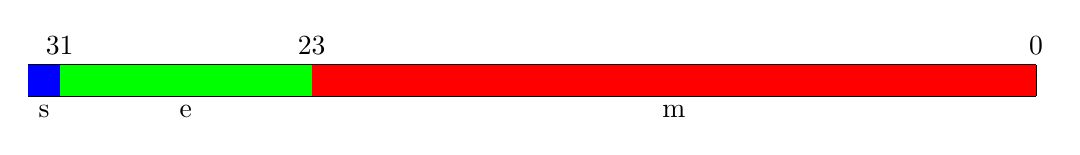
\begin{tikzpicture}
      \draw[step=0.4cm, black,  thin] (0, 0) grid (12.8, 0.4);   
     \fill [blue](0,0) rectangle(0.4,0.4);
     \fill [green](0.4,0) rectangle(3.6,0.4);
     \fill [red](3.6,0) rectangle(12.8,0.4);
     \draw (0.2,0) node[below] {s}  ;
     \draw (2,0) node[below] {e}  ;
     \draw (8.2,0) node[below] {m}  ;
     \draw (0.4,0.4) node[above]{31};
     \draw (3.6,0.4) node[above]{23};
     \draw (12.8,0.4) node[above]{0};
\end{tikzpicture}
\caption{Binary32}
\label{fig:B32}
\end{figure}
\begin{figure}[H]
    \centering
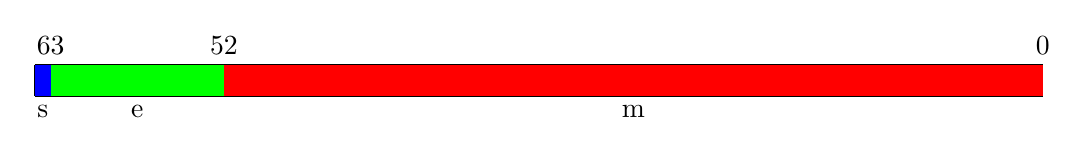
\begin{tikzpicture}
     \draw[step=0.4cm, black,  thin] (0, 0) grid (12.8, 0.4);   
     \fill [blue](0,0) rectangle(0.2,0.4);
     \fill [green](0.2,0) rectangle(2.4,0.4);
     \fill [red](2.4,0) rectangle(12.8,0.4);
     \draw (0.1,0) node[below] {s}  ;
     \draw (1.3,0) node[below] {e}  ;
     \draw (7.6,0) node[below] {m}  ;
     \draw (0.2,0.4) node[above]{63};
     \draw (2.4,0.4) node[above]{52};
     \draw (12.8,0.4) node[above]{0};
\end{tikzpicture}
\caption{Binary64}
\label{fig:B64}
\end{figure}
\begin{figure}[H]
    \centering
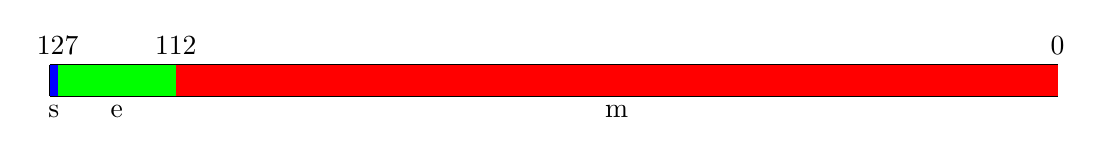
\begin{tikzpicture}
     \draw[step=0.4cm, black,  thin] (0, 0) grid (12.8, 0.4);   
     \fill [blue](0,0) rectangle(0.1,0.4);
     \fill [green](0.1,0) rectangle(1.6,0.4);
     \fill [red](1.6,0) rectangle(12.8,0.4);
     \draw (0.05,0) node[below] {s}  ;
     \draw (0.85,0) node[below] {e}  ;
     \draw (7.2,0) node[below] {m}  ;
     \draw (0.1,0.4) node[above]{127};
     \draw (1.6,0.4) node[above]{112};
     \draw (12.8,0.4) node[above]{0};
\end{tikzpicture}
\caption{Binary128}
\label{fig:B128}
\end{figure}     
We also have \textbf{Binary80} which is an \textbf{extended double precision} and two others possible formats for base of $10$:
 \begin{itemize}
     \item  \textbf{decimal64} is stored on $64$ bits.
     \item  \textbf{decimal128} is stored on $128$ bits.
 \end{itemize}
In \textbf{C} programming, \textbf{Binary32} represents \textbf{Float}, \textbf{Binary64} is \textbf{Double}, \textbf{Binary80} is \textbf{long-double} and \textbf{Binary128} is \textbf{float128}.\\
Throughout our research, we will only use \textbf{Binary64}.\\
The real numbers are transformed into a floating number and we need to round them.\\
According to the \textbf{IEEE 754} standard, there are four rounding modes among them, three are direct rounds:
\begin{itemize}
    \item \textbf{RNDN}: Rounding to nearest.\\
    It has two possibilities and the only difference between them is if the number falls in the midway.
    \begin{itemize}
        \item \textbf{Ties to even}:
         it rounds to the nearest even floating number.
        \item \textbf{Ties to away}:
        it rounds the nearest to the largest absolute value.  
    \end{itemize}
    \item \textbf{RNDZ}: Directed Rounding to $0$ (truncation).
    \item \textbf{RNDU}: Directed Rounding to $+\infty$ (rounding up or ceiling).
    \item \textbf{RNDD}: Directed Rounding to $-\infty$ (rounding down or floor).
\end{itemize}

The examples below shows us the four rounding modes.\\
\begin{table}[hbtp]
        \centering
    $$\begin{tabular}{|c|c|c|}
    \hline
    Real Number & +140.8215064611465 & +665.5752955525412\\
    \hline
    RNDN(Ties to even) & +140.821506461146 & +665.575295552541\\
    \hline
    RNDN(Ties to away) & +140.821506461147 & +665.575295552541\\
    \hline
    RNDZ & +140.821506461146 & +665.575295552541\\
    \hline
    RNDU & +140.821506461147 & +665.575295552542\\ 
    \hline
    RNDD & +140.821506461146 & +665.575295552541\\
    \hline
    \end{tabular}$$
        \caption{roundings with positive reals}
        \label{tab:positive reals}
    \end{table}
    
\begin{table}[hbtp]
        \centering   
$$\begin{tabular}{|c|c|c|}
    \hline
    Real Number & -140.8215064611465 & -665.5752955525412\\
    \hline
    RNDN(Ties to even) & -140.821506461146 & -665.575295552541\\
    \hline
    RNDN(Ties to away) & -140.821506461147 & -665.575295552541\\
    \hline
    RNDZ & -140.821506461146 & -665.575295552541\\
    \hline
    RNDU & -140.821506461146 & -665.575295552541\\ 
    \hline
    RNDD & -140.821506461147 & -665.575295552542\\
    \hline
    \end{tabular}$$ \\
\caption{roundings with negative reals}
   \label{tab:negative reals}     
    \end{table}
 
 We have the special values:
\begin{itemize}
    \item there exist two $0$: $+0$ and $-0$
    \item Infinity : $-\infty$ and $+\infty$
    \item NaN (Not a Number): result of the invalid operations.(for example :$0/0$, $\sqrt{-7}$,..)
    \item \textbf{Subnormal} Number: it is a number which has as exponent $=0$ and a pseudo-mantissa. (difference between the Mantissa and the pseudo-mantissa those which does not have a hidden $1$)
    \item   \textbf{Overflow} : according to \cite{belaid2013resolution} \enquote{This exception is caused when the result is too large in absolute value to be represented}.     
    \item \textbf{Underflow} : according to \cite{belaid2013resolution}  \enquote{This exception is caused when the actual result is too small in absolute value to be represented in the chosen format}. 
\end{itemize} 

\begin{defin}: \textbf{ulp(x)} \\
 According to \textbf{William Kahan} ($1960$) in \cite{muller2010handbook} The original definition of $ulp()$ by  \enquote{$ulp(x)$ is the gap between the two floating-point numbers nearest to $x$, even if $x$ is one of them}.\\
 $ulp(x)$ is the acronym of \textbf{Unit of the Last Place}. \\
 In the following we will use \textbf{Goldberg}'s definition:\\
Let $x$ a \textbf{floating-point} number, $x = d_0d_1d_2d_3d_4...d_{p-1}\beta^e$. we therefore have an error to represent it :$\lvert d_0d_1d_2d_3d_4...d_{p-1} - \frac{x}{\beta^e} \rvert $ which is the unit of the place.
\end{defin}

\begin{coroll}
If $x$ is a \textbf{floating-point} number, so we have :
$$ulp(x) \le 2^{-52} \lvert x \rvert$$.
\end{coroll}
\newpage

\section{Necessary tools}

\subsection{properties}
The properties are from \cite{muller2010handbook}.

\begin{prope}\label{prop:1} 
 If $X = RNDN(x)$ $\Rightarrow$ $\vert X - x \rvert \le \frac{1}{2}ulp(x)$
\end{prope}

\begin{prope} \label{prop:2} 
If $X = RNDN(x)$ $\Rightarrow$ $\vert X - x \rvert \le \frac{1}{2}ulp(X)$
\end{prope}

\begin{prope} \label{prop:3} 
If $X \in \{ RNDD(x), RNDU(x), RNDN(x)\} $ $\Rightarrow$ $\vert X - x \rvert \le ulp(x)$
\end{prope}

\begin{prope} \label{prop:4}
If $X \in \{ RNDD(x), RNDU(x), RNDN(x)\} $ $\Rightarrow$ $\vert X - x \rvert \le ulp(X)$
\end{prope}

\begin{prope}
If $x>0$ then $RNDZ(x)=RNDD(x)$.\\
If $x<0$ then $RNDZ(x)=RNDU(x)$.
\end{prope}
We need to calculate the relative error to know the accuracy of
our algorithms.\\

\begin{coroll}  
If $\lvert X - x \rvert \le \alpha. ulp(x)$  with $\alpha \in   \mathbf{R}$ $\Rightarrow$ $\frac{\lvert X - x \rvert}{\lvert x \rvert} \le \alpha.2^{-52}$
$\Rightarrow$\\ 
$\lvert X \rvert \le \lvert x \rvert (1 + \alpha.2^{-52})$.
\end{coroll}

\begin{proof} \color{-yellow}
We suppose $\lvert X - x \rvert \le \alpha. ulp(x)$,  as $ulp(x) \le 2^{-52}.\lvert x \rvert$ so we have:
$$\lvert X - x \rvert \le \alpha.2^{-52}.\lvert x \rvert$$
$$\frac{\lvert X - x \rvert}{\lvert x \rvert} \le \alpha.2^{-52}$$
According to the triangle inequality, we have that $\lvert X - x \rvert \ge \lvert X \rvert - \lvert x \rvert$ $\Rightarrow$
$$\lvert X \rvert - \lvert x \rvert \le \alpha.2^{-52}.\lvert x \rvert$$
$$\lvert X \rvert   \le \alpha.2^{-52}.\lvert x \rvert + \lvert x \rvert$$
$$\lvert X \rvert   \le \lvert x \rvert (1+\alpha.2^{-52}).$$
\end{proof}

Also need to calculate with $ulp(X)$ 
\begin{coroll}\label{cor1}
If $\lvert X - x \rvert \le \alpha. ulp(X)$  with $\alpha \in   \mathbf{R}$ $\Rightarrow$ $\lvert X \rvert \le  \vert x \rvert  + \alpha. ulp(X)$.
\end{coroll}

\begin{proof} \color{-yellow}
We suppose $\lvert X - x \rvert \le \alpha. ulp(x)$,  as $ulp(X) \le 2^{-52}.\lvert X \rvert$ so we have:
$$\lvert X - x \rvert \le \alpha.2^{-52}.\lvert X \rvert$$
$$\frac{\lvert X - x \rvert}{\lvert X \rvert} \le \alpha.2^{-52}$$
According to the triangle inequality, we have that $\lvert X - x \rvert \ge \lvert X \rvert - \lvert x \rvert$ $\Rightarrow$
$$\lvert X \rvert - \lvert x \rvert \le \alpha.2^{-52}.\lvert X \rvert$$
$$\lvert X \rvert   \le  \lvert x \rvert + \alpha.2^{-52}.\lvert X \rvert$$


\end{proof}

According to the collary \ref{cor1}, we have that $ulp(x) \le 2^{-52} .\lvert x \rvert $ then $ulp(1) = 2^{-52}$.\\
\ \\
The notations of the next part which are drawn from \cite{muller2010handbook}, we will simplify the calculations of precisions of our algorithm using \textbf{unit Roundoff}. \\
\subsection{Unit Roundoff} \label{sub:U}
The \textbf{unit Roundoff} has as \textbf{base} $2$ and as \textbf{precisions} $53$, so we have that:
$$
u = \left\{
\begin{array}{ll}
    \frac{1}{2}.ulp(1) = \frac{1}{2}.2^{-52} = 2^{-53}& for \  \ RNDN \\
    \ & \ \\
     ulp(1) = 2^{-52} & for \  \ (RNDU, RNDZ, RNDD)
\end{array}
\right.
$$

We can do only one calculation and at the end, we can replace $u$ by its values for each rounding mode.\\
\begin{coroll}\label{cor:U}
If $X=\circ(x)$ according to the properties \ref{prop:1}, \ref{prop:2}, \ref{prop:3} and \ref{prop:4} , we have his results:
\begin{itemize}
    \item $\lvert X - x \rvert \le u. \lvert x \rvert$
    \item $\lvert X - x \rvert \le u. \lvert X \rvert$
\end{itemize}
\end{coroll}

\begin{coroll}\label{cor:ux}
If $X = \circ(x)$   $\Rightarrow$ $\lvert X \rvert \le \lvert x \rvert (1 + \epsilon)$ with $\lvert \epsilon \rvert \le u$.
\end{coroll}

\begin{coroll} \label{coroll:UX}
If $X = \circ(x)$   $\Rightarrow$ $\lvert X \rvert \le \lvert x \rvert +   \epsilon$ with $\lvert \epsilon \rvert \le u . \lvert X \rvert$.
\end{coroll}
To proof the exactness of our operation, we use \textbf{Sterbenz}’s lemma.\\
The next subsection is taken from \cite{muller2010handbook}.
\subsection{\textbf{Sterbenz}’s lemma}
\begin{lemma}[\textbf{Sterbenz}]\label{lem:ster}
In a \textbf{radix\footnote{base}-$\beta$} floating-point system with \textbf{subnormal} numbers available, if $x$ and $y$ are finite \textbf{floating-point} numbers such that
$\frac{y}{2} \le x \le 2.y$ , then $x - y$ is exactly representable.
\end{lemma}
$\beta = 2$ for our research.\\
Lemma of \textbf{Sterbenz} implies for the $4$ rounding modes so the result is exact.
\begin{proof} \color{-yellow}
According to the technique of proof of Sterbeinz's lemma from \cite{muller2010handbook}.\\
We suppose that $ x \ge 0 $, $y \ge 0$ and $y \le x \le 2.y$.\\ 
Let $x = M_x.\beta^{e_x-p+1}$ and $y = M_y.\beta^{e_y-p+1}$ with their \textbf{exponents} ($e_x, e_y)$ and their \textbf{mantissa} $(M_x, M_y)$. We have:\\
$$\left\{
\begin{array}{l}
    e_{min}\le e_x \le e_{max} \\
    \ \\
    e_{min}\le e_y \le e_{max} \\
     \ \\
    0 \le M_x \le \beta^p-1 \\
    \ \\
    0 \le M_y \le \beta^p-1
\end{array}
\right.
$$

Firstly, we assume that $e_y \le e_x$, we define $\lambda = e_x - e_y$.
So we have : 
$$ x-y = (M_x.\beta^{\lambda} -M_y).\beta^{e_y-p+1}$$
We define $M = M_x.\beta^{\lambda} -M_y$.\\
According to the conditions at the beginning of the proof, we have:\\
\begin{itemize}
    \item $x\ge y$ $\Rightarrow$ $x-y \ge 0$ $\Rightarrow$ $M.\beta^{e_y-p+1} \ge 0$ as $\beta^{e_y-p+1} >0$ $\Rightarrow$ $M \ge 0$.
    \item $x\le 2.y$ $\Rightarrow$ $x-y \le y$ $\Rightarrow$ $M.\beta^{e_y-p+1} \le M_y.\beta^{e_y-p+1}$ $\Rightarrow$ $M \le M_y \le \beta^p - 1$
\end{itemize}
Secondly, we suppose that $M_y < M_x$ and that $e_y > e_x$, we define an other $\lambda=e_y - e_x $.
$$ x-y = (M_x -M_y.\beta^{\lambda}).\beta^{e_x-p+1}$$
We define $M = M_x -M_y.\beta^{\lambda}$.\\
According to the conditions at the beginning of the proof, we have:\\
\begin{itemize}
    \item $x\ge y$ $\Rightarrow$ $x-y \ge 0$ $\Rightarrow$ $M.\beta^{e_x-p+1} \ge 0$ as $\beta^{e_x-p+1} >0$ $\Rightarrow$ $M \ge 0$.
    \item $x\le 2.y$ $\Rightarrow$ $x-y \le y$ $\Rightarrow$ $M.\beta^{e_x-p+1} \le M_y.\beta^{e_y-p+1}$ $\Rightarrow$ $M \le M_y \le \beta^p - 1$
\end{itemize}
We have for our $2$ cases, the same result that is $x-y = M.\beta^{e-p+1}$ with  $e_{min}\le e_x \le e_{max}$ and $M \le \beta^p-1$.\\
We have proved that $x-y$ is  a floating point number so the calculation is exact.
\end{proof}

\section{Notations}
\begin{itemize}
    \item Function names are composed of $3$ letters followed by $3$ numbers.
If we have $Add$ then it's an addition and if we have $Mul$ then it's a multiplication.\\ 
The first $2$ numbers of the $3$ represent the argument and the last number represent the output of this function.
The number $1$ is a \textbf{Double} number, $2$ is a \textbf{Double-Double} and $3$ is a \textbf{Triple-Double}.
\item $RNDN$, $RNDU$, $RNDD$ and $RNDZ$ will be rounded as explained before.(table \ref{tab:positive reals} and table \ref{tab:negative reals})

\item $\circ()$ will represent all roundings. 

\item $cr\log_{fast-path}$, $cr\log_{accurate-path}$ and $cr\log_{advanced-accurate-path}$ for the sake of writing, we will change them to $cr\log_{fast}$, $cr\log_{accurate}$ and $cr\log_{advanced}$.

\item  \textbf{Double-Double} is a pair of \textbf{Double} numbers, \textbf{Triple-Double} is a triple of \textbf{Double} numbers.

\end{itemize}


In our research, we use as base $\beta = 2$,  precision $p = 53$ , $bias = 1023$ , $E_{min} = -1022$  and  as $E_{max} = 1023$.\\
The next chapter will be devited to calculate $cr\log$. 

%%% steps to implements cr_log 
\chapter{Steps to calculate crlog}
Before starting to implement $cr\log$, we will see what are its 
steps.\\
According to \cite{le2016computing}, first, we filter the special cases. Then, we
 reduce the argument range. After, we use the polynomial approximation and 
 evaluation.

\section{Special cases}
In the special cases, we have five possibilities:
\begin{itemize}
    \item input is $NaN$ return $NaN$
    \item Input is negatif return $NaN$
    \item Input is $+0$ or $-0$ return $-\infty$
    \item Input is $+\infty$ return $+\infty$
    \item Input is a \textbf{subnormal} number. We transform it into \textbf{normal} number then we calculate as if it is normal.
\end{itemize}

\section{Argument reduction}
We know that $\log(x.y) = \log(x) + \log(y)$. 
We have in $Input = 2^E \times m$ with $E$ is the \textbf{exposant} and $m$ is the \textbf{mantissa}.\\
So we have $\log(Input) = E \times \log(2) + \log(m)$. \\
First, we calculate $\log(m)$ with \textbf{Tang}'s algorithm and \textbf{Gal}'s algorithm.

%%%%%%%%% explanation of the algos used to reduce the argument %%%%%%%%
\subsection{ \textbf{Tang}'s Algorithm} \label{subsection:Tang}
With $x=m*2^e$ and so that $\log(x) = \log(m) +e*\log(2)$\\
First, we  calculate $\log(m)$ with \textbf{Tang}'s Algorithm (\cite{le2016computing}) .\\
We have  two possibilities: either we make a single reduction or two reductions with this algorithm.\\

\begin{figure}[H]
    \centering
    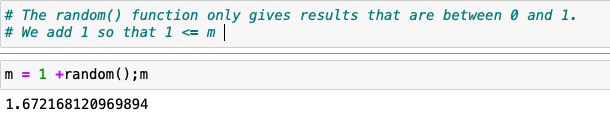
\includegraphics[width=\textwidth]{images/approche_de_Tang/Tang_intro.png}
    \caption{$m$ taken in random to test}
\end{figure}

\subsubsection{\textbf{Tang}'s algorithm with a single reduction}
We have :  $1 \le m < 2$ and we want to reduce $\log(m)$ using \textbf{Tang}'s algorithm.\\
First , we  use $k$ significant bits after the initial $1$. Then, we  take $i$ which represents the integer of the $k$ bits:\\
So we have:  $0 \le i < 2^k$ et $1+\frac{i}{2^k} \le m < 1 +\frac{i+1}{2^k}$\\
We look for $\alpha_i$ such as $1 \le m * \alpha_i < 1+\epsilon_i$ with $\epsilon_i$ as small as possible.
We can write $m = \frac{m * \alpha_i}{\alpha_i}$ and therefore have $\log(m) = \log(m * \alpha_i) - \log(\alpha_i)$.
After calculation, we have $\alpha_i = \frac{2^k}{2^k+i}$ and $\epsilon_i = \frac{1}{2^k+i}$ as $0 \le i < 2^k$ then the value $max(\epsilon_i) = \frac{1}{2^k}$.

If we take $m^{'} =  m * \alpha_i$, so we have $1 \le m^{'} < 1+\frac{1}{2^k}$. At the end of this algorithm,  $m^{'}$ has it's $k$ first zero bits after the initial $1$.

The value to be calculated has been reduced to $\log(m) = \log(m^{'}) - \log(\alpha_i)$ with $-\log(\alpha_i)$ which is already calculated and memorized in a table.\\

\begin{figure}[H]
    \centering
    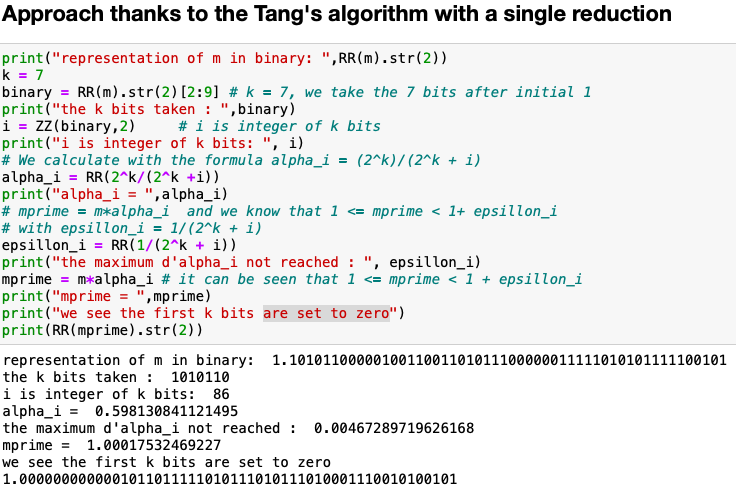
\includegraphics[width=\textwidth]{images/approche_de_Tang/Tang_1.png}
    \caption{The first reduction with $k = 7$}
\end{figure}


\subsubsection{\textbf{Tang}'s algorithm with two reductions}

After the first reduction explained above, another reduction is made again with the same value of $k$ for the following bits of the first reduction. Then, we  take $j$ which represents the integer of the $k$ bits. So we have : $0 \le j < 2^k$ and $1+\frac{j}{2^{2k}} \le m^{'} < 1 +\frac{j+1}{2^{2k}}$.

Now, we are looking for $\beta_j$ such as $1 \le m^{'} * \beta_j < 1+\epsilon^{'}_j$ with $\epsilon^{'}_j$ as small as possible. We have that $\log(m^{'})= \log(m^{'}*\beta_j) - \log(\beta_j)$.\\
After calculation : $\beta_j = \frac{2^{2k}}{2^{2k}+j}$ and $\epsilon^{'}_j = \frac{1}{2^{2k}+j}$. \\
As we have $m^{"} = m^{'}*\beta_j $ then $1 \le m{"} < 1 + \frac{1}{2^{2k}}$ .\\
So, we have $\log(m) = \log(m^{"}) - \log(\beta_j) - \log(\alpha_i)$.\\ 
$(-\log(\alpha_i))$  and  $(-\log(\beta_j))$ are already calculated and are put into memory in a table.
\begin{figure}[H]
    \centering
    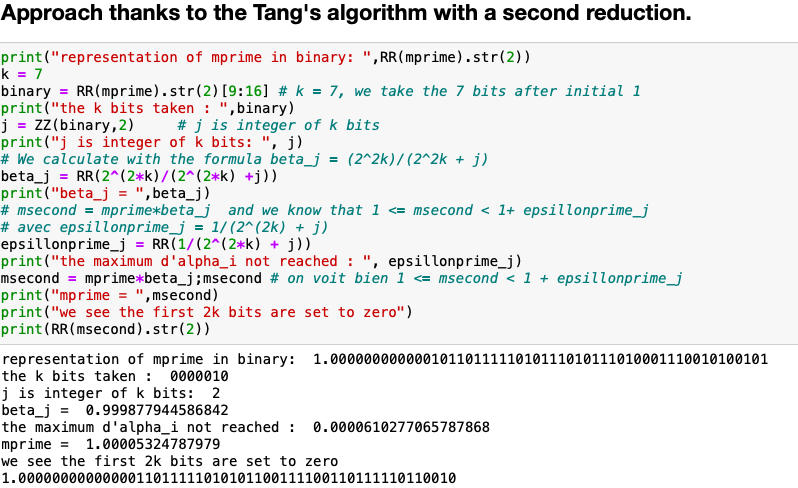
\includegraphics[width=\textwidth]{images/approche_de_Tang/Tang_2.png}
    \caption{The second reduction with $k = 7$}
\end{figure}

\subsection{\textbf{Gal}'s method with double precision}
\textbf{Gal}'s method is taken from \cite{gal1986computing}.\\
We have $x = y*2^n$ with $n$ integer and $0.75 \le y <1.5$\\ 
So  $\log(x) = \log(y)+n*\log(2)$.\\
We calculate $\log(y)$ using a table of triplets ($X_i$,\ $\log(X_i)$,\ $\frac{1}{X_i}$) with $0 \le i \le 192$.\\
$X_i = 0.75 + \frac{i}{256}+ \frac{1}{512} + E_i$ (with $E_i$ a very small number).\\
$\log(y) = \log(\frac{X_i*y}{X_i})  = \log(X_i)+\log(1+\frac{y-X_i}{X_i})= \log(X_i) + \log(1+z)$\\
If $X_i$ is choosen close to $y$, we have $\frac{-1}{384} < z < \frac{1}{384}$\\
and if more $y$ is close to 1 so $\frac{-1}{512} < z < \frac{1}{512}$.\\
We use an approximation polynomial $p(z)$ of degree $6$ (for double precision) to approach the function $\log(1+z)$.\\
If $x$ is close to $1$ so we use an approximation polynomial of $\log(x)$ without the table with a relative error of $2^{-72}$ which is negligible.\\
The table of the triplets ($X_i$, $\log(X_i)$, $\frac{1}{X_i}$) contains $576$ elements.\\
$F_i = \log(X_i)$ and $G_i = \frac{1}{X_i}$ with $0 \le i \le 192$.

The numbers $X_i$ are choosen so that $F_i$ and $G_i$ are $56$ bits of mantissa. And they have a relative precision of $2^{-65}$.\\
We search to be close to $0,75 +\frac{i}{256} + \frac{1}{512}$ with $X_i$ such that bits $57$ to $67$ of the mantissa of $\log(X_i$) and of $\frac{1}{Xi}$ which will be reset either all to $0$ or all to $1$. That's why small numbers $E_i$ were introduced. $F_i$ and $G_i$ are  the numbers with double precision obtained by a calculation of extended precisions and a symmetric rounding. 

\subsection{method with \textbf{Tang} algorithm and \textbf{Gal} method}
Our routine involves the two algorithms seen previously.\\
We start using \textbf{Tang}'s algorithm.\\
at the beginning as explained in \ref{subsection:Tang}, we only have $x=m*2^e$ and therefore we have $\log(x) = \log(m) +e*\log(2)$.\\
As mentioned in \ref{subsection:Tang}, we recover  $\alpha_i$ with the calculation:\\
$\alpha_i = \frac{2^k}{2^k+i}$ except for the following we will take $\alpha^{'}_i$ a double close to  $\alpha_i$ such that the $\log(\alpha^{'}_i)$ is the closest to a double .\\
This $\epsilon_i$ will be used to search for the $\log(\alpha^{'}_i)$ such that the bits from $54^{th}$ to $71^{st}$  are identical. (To have an approximation approximately  $2^{-71}$). (Figure \ref{fig:tang-gal})\\


\begin{figure}[H]
    \centering
    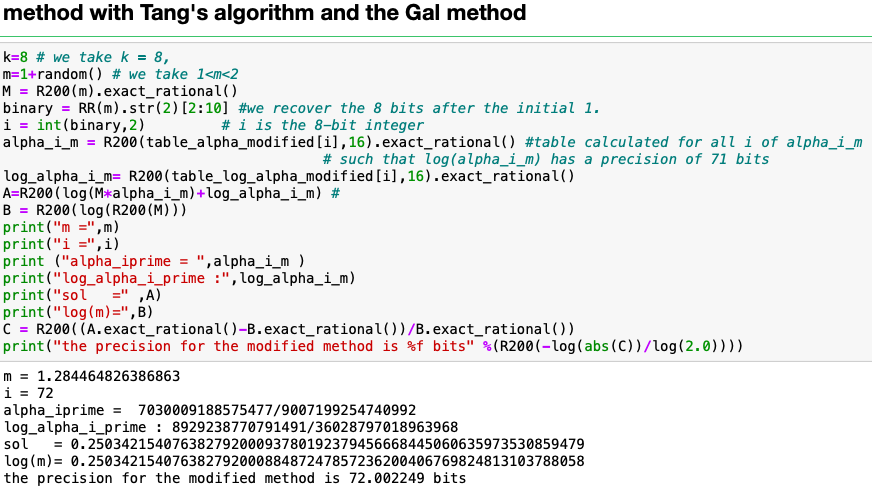
\includegraphics[scale = 0.49]{images/notre_met_Tang_Gal/algo_Tang_Gal.png}
    \caption{The revised method of \textbf{Tang} and \textbf{Gal}}\label{fig:tang-gal}
\end{figure}

We are going to verify if we obtain the same result with the \textbf{Tang} algorithm and our modified method (Figure \ref{fig:met_tang-gal}).
\begin{figure}[H]
    \centering
    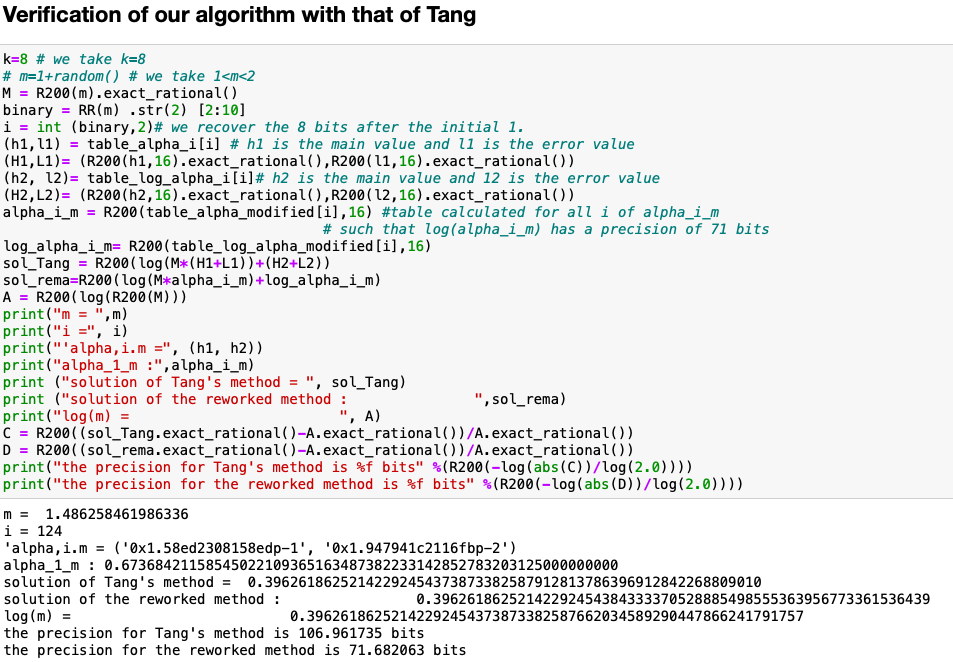
\includegraphics[scale = 0.46]{images/notre_met_Tang_Gal/algo_remanie.png}
    \caption{Verification of the revised method and \textbf{Tang}'s method}\label{fig:met_tang-gal}
\end{figure}

\section{polynomial approximation and evaluation}

Before calculating the approximation function with the \textbf{Sollya} tool, we will look for the interval for which the polynomial will be effective
for $m*\alpha^{'}_i$\\ with $0\le i<256$ and $1+\frac{i}{256}\le m < 1+\frac{i+1}{256}$ .
The calculations are experimented on \textbf{sage}, see the diagram \ref{fig:poly}:
\begin{figure}[H]
    \centering
    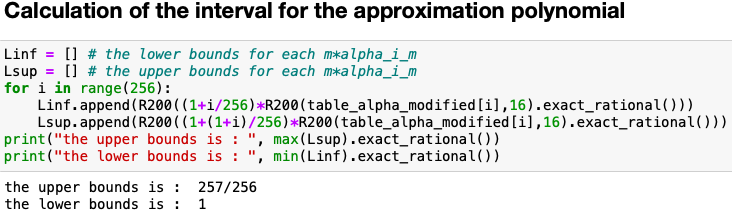
\includegraphics[scale = 0.49]{images/notre_met_Tang_Gal/calcul_intervalle.png}
    \caption{Interval calculation for the approximation polynomial }\label{fig:poly}
\end{figure}
We find as result $1 < m.\alpha^{'}_i < \frac{257}{256}$, exactly the same bounds as we calculated with the \textbf{Tang} method.\\
At the end of the calculation of the modified algorithm  from Tang and Gal's algorithm, we have that $\log(input) = \log(m.\alpha_i) - \log(\alpha_i) + E.\log( 2)$. We transform $ \log(m.\alpha_i)$ into $\log(1+t)$ to use the approximation function; then we have $t = m.\alpha_i-1$.\\
We search the polynomial approximation for $\log(1+t)$ thanks to the \textbf{Taylor} formula.\\ 
Let $P(t)$ the polynomial approximation for $\log(1+t)$, we have $P(t) \approx t - \frac{t^2}{2}...$, in case we have a constant term, we can reduce it to $0$.\\
This calculation  will be done thanks to the \textbf{Sollya} tool with its \textbf{fpminimax} function with the calculated interval.\\
Then we evaluate this approximation function with the argument $t = m.\alpha_i-1$.\\
Now, we have the operation $\log(input) = P(m.\alpha_i-1) - \log(\alpha_i )$(Figure \ref{fig:P}).\\

\begin{figure}[H]
    \centering
    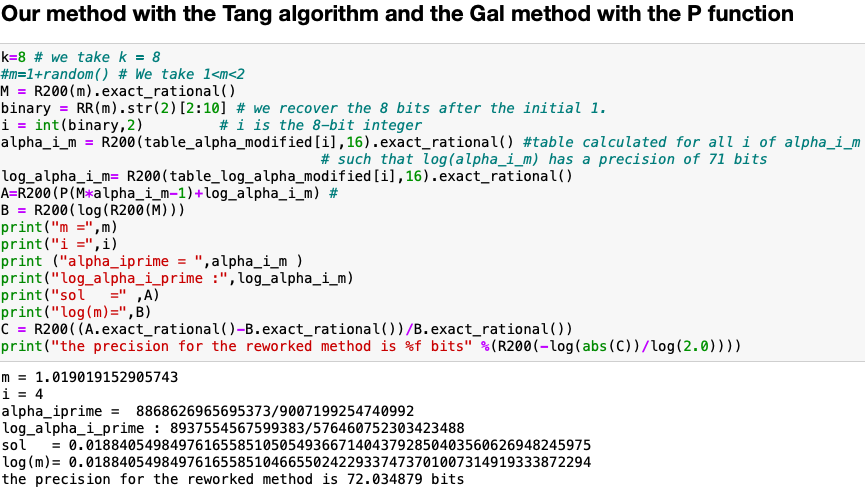
\includegraphics[scale = 0.49]{images/notre_met_Tang_Gal/algo_remanie_avec_P.png}
    \caption{The revised method  of \textbf{Tang} and \textbf{Gal} with $P(t)$}\label{fig:P}
\end{figure}

Before talking about the implementation of $cr_{\log}$, we will first see 
the used algorithms.\\

The algorithms of the chapter $4$ and chapter $5$ are taken from \cite{daramy2009cr} and \cite{lauter2005basic}.

\chapter{Operators on Double-Double numbers}
%% Sous-partie Additions double-double%%
\section{Addition Operators}

\subsection{Add112}

See algorithm \ref{algo:Add112}
\begin{lem}[Add112]\label{lem:add112}
Let $a$ and $b$  floating point numbers, with $\lvert a \rvert \ge \lvert b \rvert $, $s$ and $t$ result of $Add112(a,b)$ for the $4$ modes of rounding, considering that there is no \textbf{overflow} so :
\begin{itemize}
 \item  $(1)$ $s+t$ is exactly equal to $a+b$.              
\item  $(2)$ $ \lvert t \rvert \le 2^{-53}\lvert s \rvert $ for $RNDN$ and $ \lvert t \rvert \le 2^{-52}\lvert s \rvert $ for direct rounding modes.
\end{itemize} 
\end{lem}

\begin{proof} \color{-yellow}
$(1)$:\\
According to the calculation technique of  \textbf{Fast2Sum algorithm} proof's (\cite{muller2010handbook}), this proof shown that for the closest rounding mode ($RNDN$).\\
We suppose that $\lvert a \rvert \ge \lvert b \rvert $ and  there is no \textbf{overflow}.\\
 We suppose $a > 0$ and $b > 0$ (respectively  $a < 0$ and $b < 0$).\\
 We take $b = b_h + b_{\ell}$ with $b_h$ a multiple of $ulp(a)$ ,$\lvert b_{\ell}\rvert
< ulp(a)$ and  $b_{\ell}$ is of the same sign that $b$ (and $b_h$).\\



Either we have $0 \le \lvert b_{\ell} \rvert  < 2^{-53}. \lvert a \rvert$ or  $ 2^{-53}. \lvert a \rvert \le\lvert b_{\ell} \rvert \le  2^{-52}. \lvert a \rvert$.\\
If $0 \le \lvert b_{\ell} \rvert  < 2^{-53}. \lvert a \rvert$ for the modes of Rounding $RNDZ$, $RNDN$ and $RNDD$ (respectively $RNDZ$, $RNDN$ and $RNDU$) then $b_{\ell}$ will be ignored
otherwise $RNDU$(respectively  $RNDD$) $b_{\ell}$ is not ignore, so  $\circ (b) = b_h + ulp(a)$;\\
If $ 2^{-53}. \lvert a \rvert \le\lvert b_{\ell} \rvert \le  2^{-52}. \lvert a \rvert$ for the modes of Rounding $RNDZ$ and $RNDD$ (respectively $RNDZ$ and 
$RNDU$) then $b_{\ell}$ will be also ignored for $RNDN$(closest round) and $RNDU$(respectively $RNDN$ and $RNDD$).\\
The first case when $b_{\ell}$ is ignored so we have $\circ (b) = b_h $.
$\Rightarrow$:
\begin{itemize}
\item $s = \circ (a+b)$ $\Rightarrow$ $s = a + b_h$
\item $z = \circ (s-a)$ $\Rightarrow$ $z = a + b_h - a$  $\Rightarrow$ $z = b_h$
\item $t = \circ (b-z)$ $\Rightarrow$ $t = b - b_h$ we have that $b = b_h+b_{\ell}$ $\Rightarrow$ $t = b_{\ell}$
\end{itemize}
So we have that $s+t = a+b_h+b_{\ell}$ $\Rightarrow$ $s+t$ is exactly equal to $a+b$.\\


The second case when $b_{\ell}$ is not ignored so we have $\circ (b) = b_h +ulp(a)$.
$\Rightarrow$ :
\begin{itemize}
    \item $s = \circ (a+b)$ $\Rightarrow$ $s = a + b_h + ulp(a)$
    \item $z = \circ (s-a)$ $\Rightarrow$ $z = a + b_h + ulp(a) - a$  $\Rightarrow$ $z = b_h + ulp(a)$
    \item $t = \circ (b-z)$ $\Rightarrow$ $t = b - (b_h+ ulp(a))$ we have that $b = b_h+b_{\ell}$ $\Rightarrow$ $t = b_{\ell} - ulp(a)$
\end{itemize}
So we have that $s+t = a+b_h+ulp(a)+b_{\ell}-ulp(a)$ $\Rightarrow$ $s+t$ is exactly equal to $a+b$.\\

We suppose $a > 0$ and $b > 0$ (respectively  $a < 0$ and $b < 0$).
We suppose that $\lvert b \rvert < ulp(a)$. Either we have $ 0 < \lvert b \rvert < 2^{-53}. \lvert a \rvert $ or  $ 2^{-53} \lvert a  \rvert \le \lvert b \rvert \le  2^{-52}. \lvert a \rvert$.\\
If $ 0 < \lvert b \rvert < 2^{-53}. \lvert a \rvert $ for the modes of Rounding $RNDZ$, $RNDN$ and $RNDD$ (respectively $RNDZ$, $RNDN$ and $RNDU$) then $b$ will be ignored
otherwise $RNDU$(respectively  $RNDD$) $b$ is not ignore, so  we have $\circ (b) =  ulp(a)$;\\
If $ 2^{-53} \lvert a  \rvert \le \lvert b \rvert \le  2^{-52}. \lvert a \rvert$ for the modes of Rounding $RNDZ$ and $RNDD$ (respectively $RNDZ$ and $RNDU$) 
then $b_{\ell}$ will be also ignored  for $RNDN$(closest round) and $RNDU$(respectively $RNDN$ and $RNDD$).\\

The first case when $b$ is ignored so we have :
\begin{itemize}
\item $s = \circ (a+b)$ $\Rightarrow$ $s = a$
\item $z = \circ (s-a)$ $\Rightarrow$ $z = a  - a$  $\Rightarrow$ $z = 0$
\item $t = \circ (b-z)$ $\Rightarrow$ $t = b - 0$  $\Rightarrow$ $t = b$
\end{itemize}
So we have that $s+t = a+b$ $\Rightarrow$ $s+t$ is exactly equal to $a+b$.\\

The second case when $b$ is not ignored so we have $\circ (b) = ulp(a)$.
\begin{itemize}
    \item $s = \circ (a+b)$ $\Rightarrow$ $s = a + ulp(a)$
    \item $z = \circ (s-a)$ $\Rightarrow$ $z = a  + ulp(a) - a$  $\Rightarrow$ $z = ulp(a)$
    \item $t = \circ (b-z)$ $\Rightarrow$ $t = b - ulp(a)$  
\end{itemize}
So we have that $s+t = a+ulp(a)+b-ulp(a)$ $\Rightarrow$ $s+t$ is exactly equal to $a+b$.\\

We suppose that $a >0$ and $b<0$ (respectively $a <0$ and $b>0$):\\
If $\lvert b \rvert \ge \lvert \frac{a}{2} \rvert$.\\
So we have:
\begin{itemize}
    \item $s = \circ (a+b)$, we have $\frac{-b}{2} \le a \le -2b$  after the \textbf{Sterbenz}'s lemma (lemma \ref{lem:ster}) , we have $s$ is exactly equal to $a+b$
    \item $z = \circ (s-a)$ $\Rightarrow$ $z =\circ ((a+b)-a)$ $\Rightarrow$ $z = \circ (b) = b$ $\Rightarrow$ $z=b$
    \item $t= \circ (b-z)$  $\Rightarrow$ $t = \circ (b-b)$ $\Rightarrow$ $t=0$
\end{itemize}
So we have, $s+t$ is exactly equal to $a+b$.\\

If $\lvert b \rvert < \lvert \frac{a}{2} \rvert$:
\begin{itemize}
    \item $s = \circ (a+b)$ $\Rightarrow$ $\frac{a}{2} < s \le \ a$ $\Rightarrow$ $\frac{a}{2} \le s \le \ 2a$
    \item $z = \circ (s-a)$ $\Rightarrow$ and  $\frac{a}{2} \le s \le \ 2a$ after the \textbf{Sterbenz}'s lemma (lemma \ref{lem:ster}) , we have $z$ is exactly equal to $s-a$.
    \item $t = \circ (b-z)$ $\Rightarrow$ $t = \circ (b - (s-a)$ $\Rightarrow$ $t = \circ(a+b -s)$  $\Rightarrow$ $t = \circ(a+(b-s))$ or $-\frac{a}{2} < b < 0$\\
    and $\frac{a}{2} \le s \le \ 2a$  $\Rightarrow$ $\frac{a}{2} -0 < s - b < 2a - (-\frac{a}{2})$ $\Rightarrow$ $\frac{a}{2}< s - b < \frac{3a}{2}$ $\Rightarrow$ $\frac{a}{2} \le s - b \le 2a$ after the \textbf{Sterbenz}'s lemma (lemma \ref{lem:ster}), we have $t$ is exactly equal to $a+b-s$.\\
\end{itemize}
We have $s+t = a+b-s+s$ $\Rightarrow$ $s+t = a+b$.\\
(By symetric, we have the same results for $a<0$ and $b>0$.)\\
The $4$ modes of rounding for $Add112$ have an exact equality between $s+t$ and $a+b$.\\

$(2)$:\\
According to Proof$(1)$ , We have $6$ possibilities for the result of $s$ and $t$:\\
\begin{itemize}

\item If $s = a+b$ and $t = 0$ so   $ \lvert t \rvert \le 2^{-53} \lvert s \rvert$ for  $RNDN$ and  $ \lvert t \rvert \le 2^{-52} \lvert s \rvert$ for the direct rounding modes.\\

\item If $s = a$ and $t =b$ ($a$ and $b$ have the same sign) with  $\lvert b \rvert < 2^{-53}.\lvert a \rvert$
$\Rightarrow$ $ \lvert t \rvert \le 2^{-53} \lvert s \rvert$ for $RNDN$ a fortiori  $ \lvert t \rvert \le 2^{-52} \lvert s \rvert$ for the direct rounding modes.\\

\item If $s=a+b_h$ and $t = b_l$ ($a$, $b_h$ and $b_{\ell}$ are the same sign). 
We suppose that $a >0$, $b_h > 0$ and $b_{\ell} > 0$.
We know that $0 \le  b_{\ell}   < 2^{-53}.  a $ 
$\Rightarrow$ $  a  >  2^{53}.  b_{\ell} $ and that $b_h$ is a multiple of 
$ulp(a)$ $\Rightarrow$ $  b_h  > 2.  b_{\ell} $. So we have $a + b_h > 2^{53}b_{\ell} + 2b_{\ell}$ $\Rightarrow$ $a + b_h > (2^{53} + 2).b_{\ell}$
or $2^{53} +2 > 2^{53}$ $\Rightarrow$ $a + b_h > 2^{53}b_{\ell}$ 
$\Rightarrow$ $s > 2^{53}.t $ $\Rightarrow$ $t \le 2^{-53}.s$ $\Rightarrow$ $ \lvert t \rvert \le 2^{-53} .\lvert s \rvert$ (and similarly if $a <0$, $b_h <0$ and $b_{\ell} < 0$).\\

\item If $s = a +ulp(a)$ and $t = b -ulp(a)$:\\
We know according to  proof($1$) that $\lvert b \rvert \le 2^{-53} \lvert a \rvert$.\\
We suppose that $a>0$ and $b>0$, so we have:\\
$t \le t+ulp(a)$ $\Rightarrow$ $t \le b - ulp(a) + ulp(a)$ $\Rightarrow$ $t \le b$ 
$\Rightarrow$ $\lvert t \rvert \le 2^{-53} \lvert a \rvert $\\
We search the upper bound of $\lvert a \rvert $ as a function of $\lvert s \rvert$:\\
$s = a+ ulp(a)$ $\Rightarrow$ $s \ge a$ $\Rightarrow$ $\lvert s \rvert \ge \lvert a \rvert $ so:\\
$\lvert t \rvert \le 2^{-53} \lvert s \rvert $ \\
(and similarly if $a<0$ and $b<0$).\\


\item If $s = a + b_h + ulp(a)$ and $t = b_{\ell} -ulp(a)$\\
We know according to  proof($1$) that $\lvert b_{\ell} \rvert \le 2^{-53} \lvert b_h \rvert$.\\
We suppose that $a>0$ and $b_h>0$, so we have:\\
$t \le t+ulp(a)$ $\Rightarrow$ $t \le b_{\ell} - ulp(a) + ulp(a)$ $\Rightarrow$ $t \le b_{\ell}$ 
$\Rightarrow$ $\lvert t \rvert \le 2^{-53} \lvert b_h\rvert $  $\Rightarrow$ $\lvert t \rvert \le 2^{-53} \lvert a +b_h\rvert $\\
We search the upper bound of $\lvert a + b_h \rvert $ as a function of $\lvert s \rvert$:\\
$s = a+ b_h +ulp(a)$ $\Rightarrow$ $s \ge a + b_h$ $\Rightarrow$ $\lvert s \rvert \ge \lvert a + b_h \rvert $ so:\\
$\lvert t \rvert \le 2^{-53} \lvert s \rvert $ \\
(and similarly if $a<0$ and $b<0$).\\

\item If $t = a+b -s$ , so  $\lvert t \rvert = \lvert a+b-s \rvert = \lvert s-(a+b) \rvert $  according to collary \ref{coroll:UX} $\Rightarrow$ :\\
$$\lvert s-(a+b) \rvert \le u.\lvert s \rvert$$ with $u$ is the \textbf{unit Roundoff}(see \ref{sub:U}).
\end{itemize}
For all cases,  we have $\lvert t \rvert \le u. \lvert s \rvert$ so for $RNDN$: $\lvert t \rvert \le 2^{-53}. \lvert s \rvert$ and for the others rounding modes: $\lvert t \rvert \le 2^{-52}. \lvert s \rvert$.
\end{proof}
\subsection{Add122}
See algorithm \ref{algo:Add122}
\begin{lem}[Add122] Let $a$ a \textbf{Double} number and $(b_h,b_{\ell})$ a \textbf{Double-Double} number, with $\lvert a \rvert \ge \lvert b_h \rvert$, $s$ and $t$ result of $Add122(a,b_h,b_{\ell})$ for the $4$ modes of rounding, considering that there is no \textbf{overflow} so:
\begin{itemize}
    
    \item $(1)$ $s+t = a+b_h+b_{\ell} + \theta$ with $\lvert \theta \rvert \le u.\lvert t \rvert$
    \item  $(2)$ $ \lvert t \rvert \le 2.u. \lvert s \rvert$
\end{itemize}
\end{lem}
$2.u = 2^{-52}$ for $RNDN$ and $2.u = 2^{-51}$ for the other rounding modes.

\begin{proof} \color{-yellow}
$(1)$ We suppose $\lvert a \rvert \ge \lvert b_h \rvert $ 
and there is no \textbf{overflow}.\\
We have:
\begin{itemize}
    \item $s+ \ell = Add112(a,b_h)$ according to Lemma \ref{lem:add112} $\Rightarrow$ $s+\ell$ is exactly equal to $a+b_h$.
    \item $t = \circ (\ell + b_{\ell})$ $\Rightarrow$ $t = \ell + b_{\ell}+ \theta$ according to the collary \ref{coroll:UX} we have $\lvert \theta \rvert \le u. \lvert t \rvert$
\end{itemize}
So, we have $s+t = a+ b_h - \ell +l+b_{\ell} + \theta_1$ $\Rightarrow$ $s+t = a+ b_h + b_{\ell} + \theta_1$ $\Rightarrow$ $s+t = a+b + \theta $ with 
$\lvert \theta \rvert \le u. \lvert t \rvert$.\\

$(2)$ We suppose $\lvert a \rvert \ge \lvert b_h \rvert $
and there is no \textbf{overflow}.\\
We have:
\begin{itemize}
    \item $t= \circ(\ell + b_{\ell})$ $\Rightarrow$ $t= \ell + b_{\ell} +  \epsilon$
    with $\lvert \epsilon \rvert \le u. \lvert t \rvert$
    \item $s+ \ell = Add112(a,b_h)$ according to Lemma \ref{lem:add112} $\Rightarrow$ $s+\ell =a+b_h$ and  $\lvert \ell \rvert \le u. \lvert s \rvert$ $\Rightarrow$
    
    $$ \lvert s + \ell \rvert \ge \lvert s  \rvert - \lvert \ell \rvert $$
    $$ \lvert s + \ell \rvert \ge \lvert s  \rvert - u.\lvert s \rvert $$
    $$ \lvert s + \ell \rvert \ge (1 - u).\lvert s \rvert $$
    $\Rightarrow$
    $$(1 - u).\lvert s \rvert \le \lvert a+ b_h \rvert$$
    $$\lvert s \rvert \le \frac{1}{1-u}.\lvert a+ b_h \rvert$$
    As $\lvert \ell \rvert \le u. \lvert s \rvert$ $\Rightarrow$
    $$\lvert \ell \rvert \le \frac{u}{1-u}.\lvert a+ b_h \rvert$$
    As $\lvert b_{\ell} \rvert \le u. \lvert b_h \rvert$ and $\lvert a \rvert \ge \lvert b_h \rvert$
    $\Rightarrow$ $\lvert b_{\ell} \rvert \le u.\lvert a \rvert $ and that $\lvert a \rvert \le 2.\lvert a+b_h \rvert$ $\Rightarrow$\\
    $$ \lvert b_{\ell} \rvert \le 2.u. \lvert a+b_h \rvert$$
    $$\lvert t \rvert \le \frac{u}{1-u}. \lvert a+b_h \rvert + 2.u. \lvert a+b_h \rvert + u . \lvert t \rvert$$
    $$(1 - u).\lvert t \rvert \le (\frac{u}{1-u}  + 2.u). \lvert a+b_h \rvert$$
    $$\lvert t \rvert \le \frac{1}{1-u}.(\frac{u}{1-u}  + 2.u). \lvert a+b_h \rvert$$
    We seek the upper bound of $\lvert a+b_h \rvert $ in function of $\lvert s \rvert$:
    $$\lvert a+b_h \rvert \le (1+u). \lvert s \rvert$$
    $\Rightarrow$
    $$\lvert t \rvert \le \frac{1}{1-u}.(\frac{u}{1-u}  + 2.u). (1+u). \lvert s \rvert$$
   $$\lvert t \rvert \le \frac{(-2.u^2+2.u).(u+1)}{(1-u)^2}.\lvert s \rvert$$  
    As $\frac{(-2.u^2+2.u).(u+1)}{(1-u)^2} \le 2.u$
    We have:
    $$\lvert t \rvert \le 2.u.\lvert s \rvert$$
\end{itemize}
\end{proof}


\begin{theo}[Relative error algorithm $Add122$ without occurring of cancellation] \label{the1:add122}
Let $a$ a \textbf{double} number and $(b_h,b_{\ell})$ a \textbf{double-double} number are the arguments of the function $Add122$:\\
If $a$ and $b_h$ are the same sign, so:\\
$$s+t = (a+b_h+b_{\ell})(1+\epsilon)$$ with $\lvert \epsilon \rvert \le 2.u^2$.
\end{theo}
$2.u^2= 2^{-105}$ for $RNDN$ and $2.u^2 = 2^{-103}$ for the other rounding modes.

\begin{proof} \color{-yellow}
According to the calculation technique of the theorem $4.2$ proof's(\cite{lauter2005basic}).\\
We have $\lvert a \rvert \ge \lvert b_h \rvert$, either $a > 0$ and $b_h > 0$ or $a < 0$ and $b_h < 0$. As they're symmetric, we only use $a > 0$ and $b_h > 0$.\\
Based on the algorithm ($Add122$), we have:\\
$t = \circ (l +b_{\ell})$ according to collary \ref{cor:ux} 
$\Rightarrow$ $t = (l+b_{\ell}).(1+\epsilon)$ with $\lvert \epsilon \rvert \le u$.\\

$$t = \ell + b_{\ell} + \delta$$
with  $\delta = (\ell   + b_{\ell}) .\epsilon$
We calculate $\lvert \delta \rvert$, so we have:\\
$$ \lvert \delta \rvert = \lvert (\ell + b_{\ell}).\epsilon$$
according to the triangle inequality, we have:

$$ \lvert \delta \rvert \le \lvert \ell  .\epsilon \rvert + \lvert  b_{\ell}.\epsilon \rvert$$
$$\lvert \delta \rvert \le \lvert \epsilon \rvert .(\lvert \ell   \rvert + \lvert  b_{\ell}\rvert)$$ 
 

Based on Lemma \ref{lem:add112}, we have $\lvert l \rvert \le u.\lvert s \rvert $ 
$\Rightarrow$ $\lvert s+\ell \rvert \ge (1-u).\lvert s \rvert$ $\Rightarrow$
$(1-u).\lvert s \rvert \le \lvert a + b_h \rvert$ $\Rightarrow$ $\lvert s \rvert \le \frac{1}{1-u}.\lvert a + b_h \rvert$ $\Rightarrow$ $\lvert \ell \rvert \le \frac{u}{1-u}.\lvert a + b_h \rvert$

So we have:
$$\lvert \delta \rvert \le  \lvert \epsilon \rvert .( \frac{u}{1-u}.\lvert a + b_h \rvert + \lvert  b_{\ell}\rvert)$$ 
we have  $\lvert b_{\ell}  \rvert \le u. \lvert b_h \rvert \le u. \lvert a \rvert \le u. \lvert a  + b_h\rvert$ $\Rightarrow$
$$\lvert \delta \rvert \le \lvert \epsilon \rvert .(\frac{u}{1-u}. \lvert a + b_h \rvert + u. \lvert a + b_h \rvert)$$ 
$$\lvert \delta \rvert \le \lvert \epsilon \rvert .\frac{-u^2+2.u}{1-u}. \lvert a + b_h \rvert $$
As $\frac{-u^2+2.u}{1-u} \le 2.u$ and $\lvert \epsilon \rvert \le u$
$\Rightarrow$
$$\lvert \delta \rvert \le 2.u^2. \lvert a + b_h \rvert $$


$$ \lvert b_{\ell} \rvert \le u.\lvert a \rvert $$

$$ \lvert b_{\ell} \rvert \le u.\lvert a + b_h\rvert $$
Now we search a lower bound for $\lvert a+b_h+b_{\ell} \rvert $ in function $\lvert a+b_h \rvert $ \\
$$ \lvert  a + b_h  + b_{\ell} \rvert \le \lvert a + b_h\rvert +  \lvert b_{\ell}\rvert$$
So we have:
$$ \lvert  a + b_h  + b_{\ell} \rvert \ge (1 - u)\lvert a + b_h\rvert $$
and we knows that $\lvert \delta \rvert \le \lvert a + b_h \rvert \times  2.u^2$ $\Rightarrow$
 $$\lvert \delta \rvert \le \lvert a + b_h + b_{\ell} \rvert (\frac{1}{1-u}).2.u^2$$
 After the calculations, we have :\\
 $$\lvert \delta \rvert \le \lvert a + b_h + b_{\ell} \rvert . \lvert \epsilon \rvert$$
 with $\lvert \epsilon \rvert \le \frac{2.u^2}{1-u} \le 2.u^2$
\end{proof}


\begin{theo}[ Relative error algorithm $Add122$ with a bounded cancellation]
Let $a$ a \textbf{Double} number  and ($b_h$, $b_{\ell}$) a \textbf{double-double} number . We have for the algorithm $Add122$ with
$a$ and ($b_h$, $b_{\ell}$) it's arguments.\\
If $a$ and $b_h$ are different sign and we suppose $\lvert b_h \rvert \le 2^{-\mu} \lvert a \rvert $ with $\mu \ge 1$.\\
So :
$$ s+t = (a+  (b_h + b_{\ell}))(1+\epsilon)$$
with $$\lvert \epsilon \rvert \le 2.u^2 .\frac{2^{-53 - \mu}}{1 - 2^{-\mu} - u} \le 2.(2.u^2) = 4.u^2$$
\end{theo}

\begin{proof} \color{-yellow}
According to the calculation technique of the theorem $4.3$ proof's(\cite{lauter2005basic}).\\
We suppose $\lvert b_h \rvert \le 2^{-\mu} \lvert a \rvert$ with $\mu \ge 1$.
First we look for the upper bound, using the results of the proof of Theorem \ref{the1:add122}. We have:\\
$$\lvert b_{\ell} \rvert \le u.\lvert b_h \rvert \le u.2^{ - \mu}\lvert a \rvert $$\\
then we search the lower bound for $\lvert a+b_h \rvert$ in function of $\lvert a \rvert$:\\
$$\lvert a + b_h \rvert \ge (1-2^{ -\mu}).\lvert a\rvert$$
So we have:
$$\lvert b_{\ell}  \rvert \le \frac{u.2^{ - \mu}}{1- 2^{-\mu}}\lvert a + b_h\rvert$$

So:
$$ \lvert \delta \rvert \le \lvert a_h + b_h \rvert .2.u^2 .\frac{u.2^{- \mu}}{1 - 2^{-\mu}} $$
Now, we search the lower bound for $\lvert a + b_h +b_{\ell} \rvert$ depending on $\lvert a + b_h \rvert$.\\
We have :

$$\lvert b_{\ell}  \rvert \le \frac{u.2^{ - \mu}}{1- 2^{-\mu}}\lvert a + b_h\rvert$$
$$\lvert a + b_h +b_{\ell} \rvert \ge  \lvert a + b_h \rvert \frac{1 - 2^{-\mu} -u}{1 - 2^{-\mu}}$$
So we have for $\lvert \delta \rvert $:
$$ \lvert \delta \rvert \le \lvert a + b_h + b_{\ell} \rvert. \frac{1 - 2^{-\mu}}{1 - 2^{-\mu} -u} .2.u^2 .\frac{u.2^{ - \mu}}{1 - 2^{-\mu}} $$
$$ \lvert \delta \rvert \le \lvert a + b_h + b_{\ell} \rvert.  2.u^2.\frac{u.2^{ - \mu}}{1 - 2^{-\mu} - u} $$
So:
$$\lvert \epsilon \rvert \le  2.u^2 .\frac{2^{-53 - \mu}}{1 - 2^{-\mu} - u}$$
As $\mu \ge 1$, we want the upper bound of $\frac{u.2^{ - \mu}}{1 - 2^{-\mu} - u}$ $\Rightarrow$
$$\frac{2^{-54}}{1/2 -2^{-52}} \le 2$$
because $ 2^{-53}\le u \le 2^{-52}$
So :
$$\lvert \epsilon \rvert \le 2.2.u^2=4.u^2$$
\end{proof}


\subsection{Add222}
See algorithm \ref{algo:Add222}
\begin{lem}[Add222]
Let $(a_h, a_{\ell})$ and $(b_h, b_{\ell})$ \textbf{Double-Double} numbers, with $\lvert a_h \rvert \ge \lvert b_h \rvert$, $s$ and $t$ result of $Add222(a_h,a_{\ell},b_h,b_{\ell})$ for the $4$ modes of rounding, considering that there is no \textbf{overflow} so:

 $$\lvert t \rvert \le 6.u.\lvert s\rvert$$

\end{lem}
$6.u = 2^{-50.4}$ for $RNDN$ and $6.u = 2^{-49.4}$ for the other rounding modes.

\begin{proof} \color{-yellow}
According to $Add222$ $\Rightarrow$:
$t = \circ(m+b_{\ell})$ (corrollary \ref{cor:ux}) $\Rightarrow$ $t \le (m+b_{\ell})(1 +\epsilon_1)$ with $\lvert \epsilon_1 \rvert \le u$.
$$\lvert t \rvert \le (\lvert m \rvert + \lvert b_{\ell} \rvert).\lvert 1 +\epsilon_1 \rvert$$
We have : $m = \circ(\ell + a_{\ell})$ $\Rightarrow$ $m = (\ell+a_{\ell}).(1 +\epsilon_2)$ with $\lvert \epsilon_2 \rvert \le u$ $\Rightarrow$.
$$\lvert t \rvert \le (\lvert (\ell+a_{\ell})(1 +\epsilon_2) \rvert + \lvert b_{\ell} \rvert).\lvert 1 +\epsilon_1 \rvert$$
After calculate, we have:
$$\lvert t \rvert \le \lvert \ell \rvert .\lvert 1 + \epsilon_1 + \epsilon_2 + \epsilon_1.\epsilon_2  \rvert  + \lvert a_{\ell} \rvert .\lvert 1 + \epsilon_1 + \epsilon_2 + \epsilon_1.\epsilon_2  \rvert + \lvert b_{\ell} \rvert.\lvert 1 +\epsilon_1 \rvert$$
As $\lvert \epsilon_1 \rvert \le u$ and $\lvert \epsilon_2  \rvert \le u$ $\Rightarrow$
$$\lvert t \rvert \le \lvert \ell \rvert .( 1 + 2.u + u^2 )  + \lvert a_{\ell} \rvert .( 1 + 2.u + u^2 ) + \lvert b_{\ell} \rvert.( 1+ u)$$
As :
$$ \lvert a_{\ell} \rvert \le u.\lvert a_h \rvert \le 2.u.\lvert a_h + b_h \rvert$$
$$\lvert b_{\ell} \rvert \le u.\lvert b_h \rvert \le u.\lvert a_h \rvert \le 2.u.\lvert a_h + b_h \rvert$$
and that $a_h+b_h = s+\ell$ $\Rightarrow$
$$\lvert t \rvert \le \lvert \ell \rvert .( 1 + 2.u + u^2 )  + 2.u.( 1 + 2.u + u^2 ).\lvert s+ \ell \rvert  + 2.u.( 1+ u).\lvert s+ \ell \rvert$$
We know that $\lvert \ell \rvert \le u.\lvert s \rvert$, after calculate, we have:
$$\lvert t \rvert \le (u^4+5.u^3+7.u^2+3.u).\lvert s\rvert$$
As $(2.u^4+9.u^3+12.u^2+5.u) \le 6.u$
$$\lvert t \rvert \le 6.u.\lvert s\rvert$$

\end{proof}

\begin{theo}[Relative error algorithm $Add222$ without occurring of cancellation]
Let ($a_h$, $a_{\ell}$) and ($b_h$, $b_{\ell}$) the \textbf{double-double} . We have for the algorithm $Add222$ with ($a_h$, $a_{\ell}$) and ($b_h$, $b_{\ell}$) it's arguments.\\
If $a_h$ and $b_h$ have the same sign, so:\\
$$ s+t = ((a_h+a_{\ell}) + (b_h + b_{\ell}))(1+\epsilon)$$
with $\lvert \epsilon \rvert \le 3.u^2$ 
\end{theo}
$3.u^2 = 2^{-104.4}$ for $RNDN$ and $3.u^2 = 2^{-102.4}$ for the other rounding modes.

\begin{proof} \color{-yellow}
According to the calculation technique of the theorem $4.2$ proof's(\cite{lauter2005basic}).\\
We have $\lvert a_h \rvert \ge \lvert b_h \rvert$, either $a_h > 0$ and $b_h > 0$ or $a_h < 0$ and $b_h < 0$. As they're symmetric, we only use $a_h > 0$ and $b_h > 0$.\\
Based on the algorithm ($Add222$), we have:\\
$t = \circ (m +b_{\ell})$ according to corollary \ref{cor:ux} 
$\Rightarrow$ $t = (m+b_{\ell})(1+\epsilon_1)$ with $\lvert \epsilon_1 \rvert \le u$.\\
$$t = (\circ (\ell+ a_{\ell})+b_{\ell})(1+\epsilon_1)$$ \\
$$t = ((\ell +a_{\ell})(1+\epsilon_2) + b_{\ell})(1+\epsilon_1)$$ with $\lvert \epsilon_2 \rvert \le u$.\\
$$t = \ell + a_{\ell} + b_{\ell} + \delta$$
with  $\delta = (\ell + a_{\ell}  + b_{\ell}) \epsilon_1 + (\ell + a_{\ell}) \epsilon_1 \epsilon_2$.\\ 
We calculate $\lvert \delta \rvert$, so we have:\\
$$ \lvert \delta \rvert = \lvert (\ell + a_{\ell} + b_{\ell})\epsilon_1 + (\ell + a_{\ell})\epsilon_1 \epsilon_2 \rvert$$
according to the triangle inequality, we have:
$$ \lvert \delta \rvert \le \lvert (\ell + a_{\ell} + b_{\ell})\epsilon_1 \rvert + \lvert (\ell + a_{\ell})\epsilon_1 \epsilon_2 \rvert$$
$$ \lvert \delta \rvert \le \lvert \ell  \epsilon_1\rvert + \lvert \ell  \epsilon_1 \epsilon_2 \rvert + \lvert (a_{\ell} + b_{\ell})\epsilon_1 \rvert + \lvert  a_{\ell}\epsilon_1 \epsilon_2 \rvert$$
$$ \lvert \delta \rvert \le \lvert \ell \rvert (\lvert \epsilon_1\rvert + \lvert   \epsilon_1 \epsilon_2 \rvert) + \lvert (a_{\ell} + b_{\ell})\epsilon_1 \rvert + \lvert  a_{\ell}\epsilon_1 \epsilon_2 \rvert$$ 

$$ \lvert \delta \rvert \le \lvert \ell \rvert .( \lvert \epsilon_1 \rvert+  \lvert \epsilon_1 \epsilon_2\rvert) + \lvert (a_{\ell} + b_{\ell}) \rvert. \lvert \epsilon_1 \rvert + \lvert  a_{\ell} \rvert.\lvert \epsilon_1 \epsilon_2 \rvert $$ 
$$ \lvert \delta \rvert \le \lvert \ell \rvert .(\lvert \epsilon_1 \rvert+  \lvert \epsilon_1 \epsilon_2 \rvert) + \lvert (a_{\ell} + b_{\ell}) \rvert .\lvert \epsilon_1 \rvert  + \lvert  (a_{\ell} + b_{\ell}) \rvert .\lvert \epsilon_1 \epsilon_2 \rvert $$ 
$$ \lvert \delta \rvert \le (\lvert \ell \rvert  + \lvert (a_{\ell} + b_{\ell}) \rvert) .\lvert \epsilon_1+ \epsilon_1 \epsilon_2 \rvert$$ 
Based on Lemma \ref{lem:add112}, we have $\lvert l \rvert \le u.\lvert s \rvert $ and as $\lvert s \rvert \le \lvert a_h + b_h \rvert $ $\Rightarrow$ $\lvert l \rvert \le u.\lvert a_h + b_h \rvert $.\\
$$\lvert \delta \rvert \le (u. \lvert a_h + b_h \rvert + \lvert a_{\ell} \rvert + \lvert b_{\ell} \rvert) .\lvert \epsilon_1+ \epsilon_1 \epsilon_2 \rvert$$
we have $\lvert a_{\ell} \rvert \le u. \lvert a_h \rvert \le u. \lvert a_h  + b_h\rvert$ and  $\lvert b_{\ell} \le u. \lvert b_h \rvert \le u. \lvert a_h  + b_h\rvert$ $\Rightarrow$
$$\lvert \delta \rvert \le (u. \lvert a_h + b_h \rvert + u. \lvert a_h + b_h \rvert + u. \lvert a_h + b_h \rvert) .\lvert \epsilon_1+ \epsilon_1 \epsilon_2 \rvert$$
$$\lvert \delta \rvert \le \lvert a_h + b_h \rvert \times  3 .u .\lvert \epsilon_1+ \epsilon_1 \epsilon_2 \rvert$$
$$\lvert \delta \rvert \le \lvert a_h + b_h \rvert \times  3 .u. ( u+ u^2)$$
$$\lvert \delta \rvert \le \lvert a_h + b_h \rvert \times  3  .( u^2+ u^3)$$

We seek the upper bound of $\lvert a_h + b_h \rvert$  in function of $ \lvert a_h + b_h + a_{\ell} + b_{\ell} \rvert $:\\
$$\lvert a_{\ell} + b_{\ell} \rvert \le \lvert a_{\ell} \rvert + \lvert b_{\ell} \rvert $$
$$ \lvert a_{\ell} + b_{\ell} \rvert \le u.\lvert a_h \rvert + u.\lvert b_h \rvert $$
$$ \lvert a_{\ell} + b_{\ell} \rvert \le 2.u.\lvert a_h \rvert $$
$$ \lvert a_{\ell} + b_{\ell} \rvert \le 2.u.\lvert a_h + b_h\rvert $$
$\Rightarrow$
$$ \lvert  a_h + b_h + a_{\ell} + b_{\ell} \rvert \ge (1 - 2.u)\lvert a_h + b_h\rvert $$
and we know that $\lvert \delta \rvert \le \lvert a_h + b_h \rvert \times  3 .( u^2+ u^3)$ $\Rightarrow$
 $$\lvert \delta \rvert \le \lvert a_h +a_l + b_h + b_{\ell} \rvert (\frac{1}{1-2.u}) 3 .( u^2+ u^3)$$
 $$\lvert \delta \rvert \le \lvert a_h +a_l + b_h + b_{\ell} \rvert (\frac{ 3.u^2+ 3.u^3}{1-2.u})$$
 but $\frac{ 3.u^2+ 3.u^3}{1-2.u} \le 3.u^2$
  we have :\\
 $$\lvert \epsilon \rvert \le 3.u^2$$
\end{proof}

\begin{theo}[ Relative error algorithm $Add222$ with a bounded cancellation]
Let ($a_h$, $a_{\ell}$) and ($b_h$, $b_{\ell}$) are the \textbf{double-double} number . We have for the algorithm $Add222$ with
($a_h$, $a_{\ell}$) and ($b_h$, $b_{\ell}$) it's arguments.\\
If $a_h$ and $b_h$ are different sign and we suppose $\lvert b_h \rvert \le 2^{-\mu} \lvert a_h \rvert $ with $\mu \ge 1$.\\
So :
$$ s+t = ((a_h+a_{\ell}) + (b_h + b_{\ell}))(1+\epsilon)$$
with $$\lvert \epsilon \rvert \le 3.u^2. \frac{1-2^{-\mu -1}}{1 - 2^{-\mu} - 2.u} \le 2.3.u^2 = 6.u^2$$
\end{theo}

\begin{proof} \color{-yellow}
According to the calculation technique of the theorem $4.3$ proof's(\cite{lauter2005basic}).\\
We suppose $\lvert b_h \rvert \le 2^{-\mu} \lvert a_h \rvert$ with $\mu \ge 1$.
First we look for the upper bound, using the results of the proof of Theorem $4.1.1$. We have:\\
$$\lvert b_{\ell} \rvert \le u.\lvert b_h \rvert \le u.2^{- \mu}\lvert a_h \rvert $$\\
then we search the lower bound:\\
$$\lvert a_h + b_h \rvert \ge (1 -2^{- \mu}).\lvert a_h\rvert$$
As $\lvert a_{\ell} \rvert \le u. \lvert a_h \rvert$ and $\lvert b_{\ell} \rvert \le u. \lvert b_h \rvert \le u.2^{-\mu}. \lvert a_h \rvert$.
$$\lvert a_{\ell}  \rvert \le \frac{u}{1- 2^{-\mu}}\lvert a_h + b_h\rvert$$
and 
$$\lvert b_{\ell}  \rvert \le \frac{u.2^{- \mu}}{1- 2^{-\mu}}\lvert a_h + b_h\rvert$$
$\Rightarrow$ 
$$u+u.2^{- \mu}\le 1 - 2^{-\mu -1}$$ because of $\mu \ge 1$\\
So:
$$ \lvert \delta \rvert \le \lvert a_h + b_h \rvert .3.u^2 .\frac{1 - 2^{-\mu -1}}{1 - 2^{-\mu}} $$
Now, we search the lower bound for $\lvert a_h +a_{\ell} + b_h +b_{\ell} \rvert $ depending on $\lvert a_h + b_h \rvert$.\\
We have:
$$\lvert a_{\ell} + b_{\ell} \rvert \le \lvert a_{\ell} \rvert + \lvert b_{\ell} \rvert$$
$$\lvert a_{\ell} + b_{\ell} \rvert \le 2.u.\lvert a_h \rvert$$
$$\lvert a_{\ell} + b_{\ell} \rvert \le \frac{2.u}{1 - 2^{-\mu}}\lvert a_h + b_h \rvert$$
$$\lvert a_h +a_{\ell} + b_h +b_{\ell} \rvert \ge  \lvert a_h + b_h \rvert \frac{1 - 2^{-\mu} -2.u}{1 - 2^{-\mu}}$$
So we have for $\lvert \delta \rvert $:
$$ \lvert \delta \rvert \le \lvert a_h + a_{\ell} + b_h + b_{\ell} \rvert. \frac{1 - 2^{-\mu}}{1 - 2^{-\mu} -2.u} .3.u^2 .\frac{1 - 2^{-\mu -1}}{1 - 2^{-\mu}} $$
$$ \lvert \delta \rvert \le \lvert a_h + a_{\ell} + b_h + b_{\ell} \rvert.  3.u^2 .\frac{1 - 2^{-\mu -1}}{1 - 2^{-\mu} - 2.u} $$
So:
$$\lvert \epsilon \rvert \le 3.u^2 .\frac{1 - 2^{-\mu -1}}{1 - 2^{-\mu} - 2.u}$$
As $\mu \ge 1$, we want the upper bound of $\frac{1 - 2^{-\mu -1}}{1 - 2^{-\mu} - 2.u}$ $\Rightarrow$
$$\frac{3/4}{1/2 -2.u} \le 2$$
So :
$$\lvert \epsilon \rvert \le 2.3.u^2 = 6.u^2$$
\end{proof}




%% Sous-partie Multiplications double-double%%
\section{Multiplication Operators}

\subsection{Mul112}
See algorithm \ref{algo:Mul112}
\begin{lem}[Mul112]
Let $a$ and $b$  floating point numbers,  $s$ and $t$ result of $Mul112(a,b)$ for the $4$ modes of rounding, considering that there is no \textbf{overflow} so :
\begin{itemize}
 \item  $(1)$ $r_1+r_2$ is exactly equal to $a.b$.              
\item  $(2)$ $ \lvert r_2 \rvert \le u.\lvert r_1 \rvert $
\end{itemize} 
\end{lem}

\begin{proof} \color{-yellow}
$(1)$
According to \cite{muller2010handbook},  $FMA(a,b,-c)$ is exacty equal to $a+b-c$ for the $4$ modes of rounding .\\
Based on Algorithm $Mul112$, we have :\\
$r_2 = FMA(a,b,-r1)$ that supposed $\Rightarrow$ $r_2 = a*b -r_1$\\
So 
$$r_1 + r_2 = a*b-r_1 +r_1$$
$$r_1 + r_2 = a*b$$

$(2)$ 
$r1 = \circ (a*b)$ according to the collary \ref{coroll:UX}
$\Rightarrow$
$r1 =  a*b +\epsilon$ with $\lvert \epsilon \rvert \le u.\lvert r_1 \rvert$
We know that $r2$ is exactly equal to $a*b -r_1$.\\
$\Rightarrow$ $r_2 = a*b -r1$ $\Rightarrow$
$$r_2 = a*b -(a*b+\epsilon)$$
$$r_2 = -\epsilon$$
That $\lvert \epsilon \rvert \le u.\lvert r_1 \rvert$ $\Rightarrow$ $\lvert r_2 \rvert \le u.\lvert r_1 \rvert $.\\
\end{proof}
\subsection{Mul122}
See algorithm \ref{algo:Mul122}
\begin{lem}[Mul122] Let $a$ a \textbf{Double} number and $(b_h,b_{\ell})$ a \textbf{Double-Double} number, $r_1$ and $r_2$ result of $Mul122(a,b_h,b_{\ell})$ for the $4$ modes of rounding, considering that there is no \textbf{overflow} so $\lvert r_2 \rvert \le u. \lvert r_1 \rvert$.
\end{lem}

\begin{proof} \color{-yellow}
We know $\lvert b_{\ell} \rvert \le u.\lvert b_h \rvert$

 In the algorithme $Mul122$, we see $r_1, r_2 = Add112(t_1, t_6)$, bases on the lemma \ref{lem:add112}, we have $\lvert r_2 \rvert \le u.\lvert r_1 \rvert$.
\end{proof}

\begin{theo}[Relative error algorithm $Mul122$]

Let $a$ a \textbf{double} number and $(b_h,b_{\ell})$ a \textbf{double-double} number are the arguments of the function $Mul122$:\\
So:
$$r_1+r_2 = (a. (b_h+b_{\ell})).(1+\epsilon)$$ with $\lvert \epsilon \rvert \le 3.u^2$.
\end{theo}

$3.u^2 = 2^{-104.41}$ for $RNDN$ and $3.u^2 = 2^{-102.41}$ for the other rounding modes.

\begin{proof} \color{-yellow}
According to the calculation technique of the theorem $4.7$ proof's(\cite{lauter2005basic}).\\
We have from Algorithm \ref{algo:Mul122}:\\
$r_1,r_2 = Add112(t_1,t_4)$ according to $Add112$ $\Rightarrow$ $r_1+r_2 = t_1+t_4$\\
$t_4 = \circ (t_2+t_3)$ $\Rightarrow$ $t_4 = (t_2+t_3)(1+\epsilon_1)$ with $\lvert \epsilon_1 \rvert \le u$\\
$t_3 = \circ (a.b_{\ell})$ $\Rightarrow$ $t_3 = (a.b_{\ell})(1+\epsilon_2)$ with $\lvert \epsilon_2 \rvert \le u$\\
$t_1,t_2 = Mul112(a,b_h)$ according to $Mul112$  $\Rightarrow$ $\lvert t_2 \rvert \le u .\lvert t_1 \rvert$ and
$t_1 + t_2 =  a \times b_h $\\
So we have :
$$t_4 = (t_2 +a.b_{\ell}.(1+\epsilon_2)).(1+\epsilon_1)$$
$$t_4 = t_2 +a.b_{\ell}+ a.b_{\ell}.\epsilon_2+ t_2.\epsilon_1 + a.b_{\ell}.\epsilon_1+ a.b_{\ell}.\epsilon_2.\epsilon_1$$
as $r_1+r_2 = t_1+t_4$ $\Rightarrow$
$$r_1+r_2 = t_1 +(t_2 +a.b_{\ell}+ a.b_{\ell}.\epsilon_2+ t_2.\epsilon_1 + a.b_{\ell}.\epsilon_1+ a.b_{\ell}.\epsilon_2.\epsilon_1) $$
but $t_1+t_2 = a.b_h$ $\Rightarrow$
$$r_1+r_2 =a.b_h +a.b_{\ell}+ a.b_{\ell}.\epsilon_2+ t_2.\epsilon_1 + a.b_{\ell}.\epsilon_1+ a.b_{\ell}.\epsilon_2.\epsilon_1 $$
$$r_1+r_2 = a.b_h+a. b_{\ell} + \delta $$ 
with 
$$\delta = t_2.\epsilon_1 + a.b_{\ell}.\epsilon_2 + a.b_{\ell}.\epsilon_1 + a.b_{\ell}.\epsilon_2.\epsilon_1$$
So we have:
$$ \lvert \delta \rvert \le \lvert t_2.\epsilon_1 \rvert + \lvert a.b_l.(\epsilon_1 + \epsilon_2 + \epsilon_2.\epsilon_1  )\rvert  $$
as we know that $\lvert \epsilon_1 \rvert \le u$ and $\lvert \epsilon_2 \rvert \le u$ $\Rightarrow$
$$ \lvert \delta \rvert \le \lvert t_2 \rvert .u + \lvert a.b_{\ell} \rvert .(u^2 +2.u)  $$
According to the conditions of the algorithm :\\
 $\lvert b_{\ell} \rvert \le u. \lvert b_h \rvert$ $\Rightarrow$
$\lvert a \times b_{\ell} \rvert \le u. \lvert a. b_h\rvert$ .   
So:
$$ \lvert \delta \rvert \le \lvert t_2 \rvert .u + u.\lvert a.b_h \rvert .(u^2 +2.u)  $$
$$ \lvert \delta \rvert \le \lvert t_2 \rvert .u + \lvert a.b_h \rvert .(u^3 +2.u^2) $$
As $a.b_h = t_1 + t_2$ and that $ \lvert t_2 \rvert \le u. \lvert t_1 \rvert$, we have  $ \lvert a.b_h \rvert \ge \lvert (1 + \frac{1}{u}) . t_2 \rvert$ but $1+ \frac{1}{u} > 0$ $\Rightarrow$
$$ (1 + \frac{1}{u}) .\lvert t_1 \rvert  \le \lvert a.b_h \rvert $$
$$  \frac{1+u}{u} .\lvert t_2 \rvert  \le \lvert a.b_h \rvert $$
$$   \lvert t_2 \rvert  \le \frac{u}{1+u}. \lvert a.b_h \rvert $$
So :
$$ \lvert \delta \rvert \le \frac{u^2}{1+u}. \lvert a.b_h \rvert  + \lvert a.b_h \rvert .(u^3 +2.u^2) $$
After calculate,
$\Rightarrow$
$$ \lvert \delta \rvert \le \frac{u^4+3.u^3+3.u^2}{1+u}. \lvert a.b_h \rvert $$
Now , we search a lower bound for $\lvert a_h .(b_h + b_{\ell}) \rvert $ in fuction of  $\lvert a_h.b_h \rvert $.\\
For to calculate this lower bound, we need to search the upper bound of $\lvert a.b_{\ell}\rvert$. So we have:
$$\lvert a.b_{\ell}  \rvert \le u.\lvert a.b_h \rvert$$
So we have:
$$\lvert a.(b_h + b_{\ell}) \rvert \ge (1 - u).\lvert a_h.b_h \rvert  $$
$$\frac{1}{1 - u}.\lvert a.(b_h + b_{\ell}) \rvert \ge \lvert a_h.b_h \rvert  $$
For the calculation of relative error, we have:
$$ \lvert \delta \rvert \le  \frac{u^4+3.u^3+3.u^2}{1-u^2} . \lvert a.b_h \rvert $$
As $\frac{u^4+3.u^3+3.u^2}{1-u^2} \le 3.u^2$
$\Rightarrow$ $\lvert \delta \rvert \le  3.u^2.\lvert a.(b_h + b_{\ell}) \lvert $.\\
For $r_1+r_2 = (a. (b_h+b_{\ell})).(1+\epsilon)$
We have that $\lvert \epsilon \rvert \le 3.u^2$
\end{proof}
\subsection{Mul222}
See algorithm \ref{algo:Mul222}
\begin{lem}[Mul222] Let $(a_h,a_{\ell})$  and $(b_h,b_{\ell})$ are  \textbf{Double-Double} numbers, $r_1$ and $r_2$ result of $Mul222(a_h,a_{\ell},b_h,b_{\ell})$ for the $4$ modes of rounding, considering that there is no \textbf{overflow} so $ \lvert r_1 \rvert \le u.\lvert r_2 \rvert $.
\end{lem}

\begin{proof} \color{-yellow}
We know $\lvert b_{\ell} \rvert \le u.\lvert b_h \rvert$\\
In the algorithme $Mul222$, we see $r_1, r_2 = Add112(t_1, t_6)$, based on the lemma \ref{lem:add112}, we have $\lvert r_2 \rvert \le u.\lvert r_1 \rvert$.
\end{proof}

\begin{theo}[Relative error algorithm $Mul222$]
Let $(a_h,a_{\ell})$  and $(b_h,b_{\ell})$ are \textbf{double-double} numbers and are the arguments of the function $Mul222$:\\
so:\\
$$r_1+r_2 = ((a_h+a_{\ell}) \times (b_h+b_{\ell}))(1+\epsilon)$$ with $\lvert \epsilon \rvert \le 7.u^2$.
\end{theo}

$7.u^2 = 2^{-103.19}$ for $RNDN$ and $7.u^2 = 2^{-101.19}$ for the other rounding modes.

\begin{proof} \color{-yellow}
According to the calculation technique of the theorem $4.7$ proof's(\cite{lauter2005basic}).\\
We have from Algorithm $7$:\\
$r_1,r_2 = Add112(t_1,t_6)$ according to $Add112$ $\Rightarrow$ $r_1+r_2 = t_1+t_6$\\
$t_6 = \circ (t_2+t_5)$ $\Rightarrow$ $t_6 = (t_2+t_5)(1+\epsilon_1)$ with $\lvert \epsilon_1 \rvert \le u$\\
$t_5 = \circ (t_3+t_4)$ $\Rightarrow$ $t_5 = (t_3+t_4)(1+\epsilon_2)$ with $\lvert \epsilon_2 \rvert \le u$\\
$t_4 = \circ (b_h \times a_{\ell})$ $\Rightarrow$ $t_4 = (b_h . a_{\ell}).(1+\epsilon_3)$ with $\lvert \epsilon_3 \rvert \le u$\\
$t_3 = \circ (a_h\times b_{\ell})$ $\Rightarrow$ $t_3 = (a_h.b_l).(1+\epsilon_4)$ with $\lvert \epsilon_4 \rvert \le u$\\
$t_1,t_2 = Mul112(a_h,b_h)$ according to $Mul112$  $\Rightarrow$ $\lvert t_2 \rvert \le u .\lvert t_1 \rvert$ and $t_1 + t_2 = a_h.b_h$\\
So we have :
$$t_6 = (t_2+((a_h . b_{\ell}).(1+\epsilon_4)+(b_h. a_{\ell}).(1+\epsilon_3)).(1+\epsilon_2)).(1+\epsilon_1)$$
As $r_1+r_2 = t_1+t_6$ $\Rightarrow$
$$r_1+r_2 = t_1 +(t_2+((a_h . b_{\ell}).(1+\epsilon_4)+(b_h. a_{\ell}).(1+\epsilon_3)).(1+\epsilon_2)).(1+\epsilon_1) $$
$$r_1+r_2 = t_1 +t_2+a_h . b_{\ell}+b_h. a_{\ell} + \delta $$ 
with 
$$\delta = t_2.\epsilon_1 +a_h.b_l.(\epsilon_4 + \epsilon_2 + \epsilon_4.\epsilon_2 + \epsilon_1 + \epsilon_4.\epsilon_1 + \epsilon_2.\epsilon_1 + \epsilon_4.\epsilon_2.\epsilon_1) +a_l.b_h.(\epsilon_3 + \epsilon_2 + \epsilon_3.\epsilon_2 + \epsilon_1 + \epsilon_3.\epsilon_1 + \epsilon_2.\epsilon_1 + \epsilon_3.\epsilon_2.\epsilon_1)  $$
So we have:
$$ \lvert \delta \rvert \le \lvert t_2.\epsilon_1 \rvert + \lvert a_h.b_l.(\epsilon_4 + \epsilon_2 + \epsilon_4.\epsilon_2 + \epsilon_1 + \epsilon_4.\epsilon_1 + \epsilon_2.\epsilon_1 + \epsilon_4.\epsilon_2.\epsilon_1) \rvert + \lvert a_l.b_h.(\epsilon_3 + \epsilon_2 + \epsilon_3.\epsilon_2 + \epsilon_1 + \epsilon_3.\epsilon_1 + \epsilon_2.\epsilon_1 + \epsilon_3.\epsilon_2.\epsilon_1) \rvert  $$
$$ \lvert \delta \rvert \le \lvert t_2.\epsilon_1 \rvert + \lvert a_h.b_l \rvert . \lvert \epsilon_4 + \epsilon_2 + \epsilon_4.\epsilon_2 + \epsilon_1 + \epsilon_4.\epsilon_1 + \epsilon_2.\epsilon_1 + \epsilon_4.\epsilon_2.\epsilon_1 \rvert + \lvert a_l.b_h \rvert . \lvert \epsilon_3 + \epsilon_2 + \epsilon_3.\epsilon_2 + \epsilon_1 + \epsilon_3.\epsilon_1 + \epsilon_2.\epsilon_1 + \epsilon_3.\epsilon_2.\epsilon_1 \rvert  $$
as we know that $\lvert \epsilon_i \rvert \le u$ with $1\le i \le 4$ $\Rightarrow$
$$ \lvert \delta \rvert \le \lvert t_2.\epsilon_1 \rvert + (\lvert a_h.b_l \rvert +\lvert a_l.b_h \rvert ). \lvert \epsilon_4 + \epsilon_2 + \epsilon_4.\epsilon_2 + \epsilon_1 + \epsilon_4.\epsilon_1 + \epsilon_2.\epsilon_1 + \epsilon_4.\epsilon_2.\epsilon_1 \rvert $$
According to the conditions of the algorithm:\\
$\lvert a_{\ell} \rvert \le u. \lvert a_h \rvert$ and $\lvert b_{\ell} \rvert \le u. \lvert b_h \rvert$ $\Rightarrow$
$\lvert a_{\ell} \times b_h \rvert \le u. \lvert a_h \times b_h\rvert$ and $\lvert a_h \times b_{\ell} \rvert \le u. \lvert a_h \times b_h\rvert$.   
So:
$$ \lvert \delta \rvert \le \lvert t_2.\epsilon_1 \rvert + (u. \lvert a_h . b_h\rvert +u \lvert a_h . b_h\rvert ). \lvert \epsilon_4 + \epsilon_2 + \epsilon_4.\epsilon_2 + \epsilon_1 + \epsilon_4.\epsilon_1 + \epsilon_2.\epsilon_1 + \epsilon_4.\epsilon_2.\epsilon_1 \rvert $$
We search the upper bound of $\lvert t_2 \rvert $ in function of $\lvert a_h.b_h \rvert$, we begin with the upper bound of $\lvert t_1 \rvert $, as $ t_1 + t_2 = a_h.b_h$ and $\lvert t_2 \rvert \le u.\lvert t_1 \rvert$, we have that:
$$\lvert t_1 + t_2 \rvert \ge (1 - u) . \lvert t_1 \rvert$$
$$\lvert t_1 \rvert \le \frac{1}{1-u}. \lvert a_h.b_h \rvert$$
and so:
$$\lvert t_2 \rvert \le \frac{u}{1-u}. \lvert a_h.b_h \rvert$$

$$ \lvert \delta \rvert \le  \frac{u}{1-u}. \lvert a_h . b_h\rvert. \lvert \epsilon_1 \rvert + 2.u. \lvert a_h . b_h\rvert . \lvert \epsilon_4 + \epsilon_2 + \epsilon_4.\epsilon_2 + \epsilon_1 + \epsilon_4.\epsilon_1 + \epsilon_2.\epsilon_1 + \epsilon_4.\epsilon_2.\epsilon_1 \rvert $$
$$ \lvert \delta \rvert \le   \lvert a_h . b_h\rvert.(\frac{u}{1-u}. \lvert \epsilon_1 \rvert + 2.u. \lvert \epsilon_4 + \epsilon_2 + \epsilon_4.\epsilon_2 + \epsilon_1 + \epsilon_4.\epsilon_1 + \epsilon_2.\epsilon_1 + \epsilon_4.\epsilon_2.\epsilon_1 \rvert) $$
After calculation,
$\Rightarrow$
$$ \lvert \delta \rvert \le   \lvert a_h . b_h\rvert.\frac{-2.u^5 - 4.u^4 + 7.u^2}{1-u}$$
Now , we search a lower bound for $\lvert (a_h + a_{\ell}).(b_h + b_{\ell}) \rvert $ in function of  $\lvert a_h.b_h \rvert $.\\
To calculate this lower bound, we need to search the upper bound of $\lvert a_h.b_{\ell} +a_{\ell}.b_h + a_{\ell}.b_{\ell} \rvert$. So we have:
$$\lvert a_h.b_{\ell} +a_{\ell}.b_h + a_{\ell}.b_{\ell} \rvert \le \lvert a_h.b_{\ell} \rvert + \lvert  a_{\ell}.b_h \rvert + \lvert a_{\ell}.b_{\ell} \rvert $$
$$\lvert a_h.b_{\ell} +a_{\ell}.b_h + a_{\ell}.b_{\ell} \rvert \le u.\lvert a_h.b_h \rvert + u.\lvert  a_h.b_h \rvert + u^2.\lvert a_h.b_h \rvert $$
$$\lvert a_h.b_{\ell} +a_{\ell}.b_h + a_{\ell}.b_{\ell} \rvert \le (u^2+2.u).\lvert a_h.b_h \rvert $$
So we have:
$$\lvert (a_h +a_{\ell}).(b_h + b_{\ell}) \rvert \ge (1 - (u^2+2.u)).\lvert a_h.b_h \rvert  $$
For the calculation of relative error, we have:
$$\lvert \delta \rvert \le   \frac{-2.u^5 - 4.u^4 + 7.u^2}{(1-u).(1 - (u^2+2.u))}.\lvert (a_h + a_{\ell}).(b_h + b_{\ell})\rvert $$
but $\frac{-2.u^5 - 4.u^4 + 7.u^2}{(1-u).(1 - (u^2+2.u))} \le 7.u^2$
$\Rightarrow$ $\lvert \delta \rvert \le  7.u^2.\lvert (a_h + a_{\ell}).(b_h + b_{\ell}) \lvert $.\\
For $r_1+r_2 = ((a_h+a_{\ell}). (b_h+b_{\ell})).(1+\epsilon)$
so $\lvert \epsilon \rvert \le 7.u^2$
\end{proof}


\chapter{Operators on Triple-Double numbers}
%% Sous-partie Additions triple-double%%
\section{Addition Operators}
\subsection{Add133}
See algorithm \ref{algo:Add133}
\begin{lem}[Add133] Let $a$ a \textbf{double} number and $(b_h, b_m, b_{\ell})$ a   \textbf{triple-Double} number, $r_h$, $r_m$ and  $r_{\ell}$ result of $Add133(a,b_h,b_m,b_{\ell})$ for the $4$ modes of rounding, considering that there is no \textbf{overflow} so $ \lvert r_{\ell} \rvert \le u. \lvert r_m \rvert$, $\lvert r_m \rvert  \le u.\lvert  r_h \rvert$ and $\lvert r_{\ell} \rvert  \le u^2.\lvert  r_h \rvert$
\end{lem}

\begin{proof} \color{-yellow}
We suppose that $\lvert b_m \rvert \le u. \lvert b_h \rvert$, $\lvert b_{\ell} \rvert \le u. \lvert b_m \rvert$, according to  $Add133$,  so we have:
\begin{itemize}
\item $r_m+r_{\ell} = Add112(t_2, t_4)$ thanks to $Add112$ $\Rightarrow$ $r_m+r_{\ell} = t_2+ t_4$ and $ \lvert r_{\ell} \rvert \le u. \lvert r_m \rvert$. 

\item $t_4 = \circ(t_3 + b_{\ell})$ $\Rightarrow$ $t_4 = (t_3 + b_{\ell}).(1+\epsilon)$ with $\lvert \epsilon \rvert \le u$.

\item $t_2+ t_3 = Add112(t_1, b_m)$ thanks to $Add112$ $\Rightarrow$ $t_2+ t_3 = t_1+ b_m$ and $ \lvert t_3 \rvert \le u. \lvert t_2 \rvert$.

\item $r_h+t_1 = Add112(a,b_h)$ thanks to $Add112$ $\Rightarrow$ $r_h+t_1 = a+b_h$ and $ \lvert t_1 \rvert \le u. \lvert r_h \rvert$ $\Rightarrow$
\end{itemize}
$$r_m+r_{\ell} = t_2+ t_4$$
$$r_m+r_{\ell} = t_2 + (t_3 + b_{\ell}).(1+\epsilon)$$
$$r_m+r_{\ell} = t_2 + t_3.(1+\epsilon)+ b_{\ell}.(1+\epsilon)$$
$$r_m+r_{\ell} = t_2 + t_3+ t_3.\epsilon + b_{\ell}.(1+\epsilon)$$
As $t_2+t_3 = t_1+b_m$ $\Rightarrow$
$$r_m+r_{\ell} = t_1+b_m+ t_3.\epsilon + b_{\ell}.(1+\epsilon)$$
$$ \lvert r_m+r_{\ell} \rvert  = \lvert  t_1+b_m+ t_3.\epsilon + b_{\ell}.(1+\epsilon) \lvert$$
$$\lvert r_m+r_{\ell} \rvert  \le \lvert  t_1+b_m \rvert + \lvert t_3.\epsilon \rvert + \lvert b_{\ell}.(1+\epsilon) \lvert$$ 
We search the lower bound of $\lvert t_3 \rvert $ in function of $\lvert  t_1+b_m \rvert$:\\
$\lvert t_1 + b_m \rvert = \lvert t_2 + t_3 \rvert $ $\Rightarrow$ $\lvert t_1 + b_m \rvert \ge (1 + \frac{1}{u}).\lvert  t_3 \rvert $ $\Rightarrow$ $\lvert t_3 \rvert \le \frac{u}{u+1}.\lvert  t_1 + b_m \rvert $
$$\lvert r_m+r_{\ell} \rvert  \le \lvert  t_1+b_m \rvert +\frac{u}{u+1}. \lvert (t_1 + b_m) .\epsilon \rvert + \lvert b_{\ell}.(1+\epsilon) \lvert$$
$$\lvert r_m+r_{\ell} \rvert  \le \lvert  t_1+b_m \rvert +\frac{u^2}{u+1}. \lvert (t_1 + b_m) \rvert + \lvert b_{\ell}.(1+ u) \lvert$$
$$\lvert r_m+r_{\ell} \rvert  \le +\frac{u^2+u+1}{u+1}. \lvert (t_1 + b_m) \rvert + \lvert b_{\ell}.(1+ u) \lvert$$ 
According to the conditions of $Add112$, we have $\lvert t_1 \rvert \ge \lvert b_m \rvert $ and also that $\lvert b_{\ell} \rvert \le u. \lvert b_m \rvert $ $\Rightarrow$
$$\lvert r_m+r_{\ell} \rvert  \le \frac{2.(u^2+u+1)+u(u+1)^2}{u+1}.\lvert  t_1 \rvert$$
$$\lvert r_m+r_{\ell} \rvert  \le \frac{u^3+4.u^2+3.u+1}{u+1}.\lvert  t_1 \rvert$$
As $ \lvert t_1 \rvert \le u. \lvert r_h \rvert $ $\Rightarrow$
$$\lvert r_m+r_{\ell} \rvert  \le u.\frac{u^3+4.u^2+3.u+1}{u+1}.\lvert  r_h \rvert$$
 We have: $\frac{u^4+4.u^3+3.u^2+u}{u+1} \le u$ $\Rightarrow$
$$\lvert r_m+r_{\ell} \rvert  \le u.\lvert  r_h \rvert$$
We know that $ \lvert r_{\ell} \rvert \le u. \lvert r_m \rvert$ $\Rightarrow$ $(1 - u). \lvert r_m \rvert \le \lvert r_m + r_{\ell} \rvert $.\\
We have :
$$(1 - u).\lvert r_m \rvert  \le u.\lvert  r_h \rvert$$
$$\lvert r_m \rvert  \le \frac{u}{1-u}.\lvert  r_h \rvert$$
But $\frac{u}{1-u} \le u$ $\Rightarrow$
$$\lvert r_m \rvert  \le u.\lvert  r_h \rvert$$
and
$$\lvert r_{\ell} \rvert  \le u^2.\lvert  r_h \rvert$$
\end{proof}

\begin{theo}[Relative error algorithm $Add133$ without occuring of cancellation]

Let $a$ a \textbf{double} number and $(b_h,b_m,b_{\ell})$ a \textbf{triple-double} number are the arguments of the function $Add133$.\\
So:\\
$$r_h +r_m +r_{\ell} = (a + (b_h+ b_m +b_{\ell})).(1+\epsilon)$$ with $\lvert \epsilon \rvert \le 3.u^3$.
\label{the1:Add133}
\end{theo}

$3.u^3= 2^{-157.41}$ for $RNDN$ and $3.u^3 = 2^{-154.41}$ for the other rounding modes.
\begin{proof} \color{-yellow}
According to the calculation technique of the theorem $4.2$ proof's(\cite{lauter2005basic}).\\
We have $\lvert a \rvert \ge \lvert b_h \rvert$, either $a > 0$ and $b_h > 0$ or $a < 0$ and $b_h < 0$. As they're symmetric, we only use $a > 0$ and $b_h > 0$.\\
We have from Algorithme \ref{algo:Add133}:\\
$r_m + r_{\ell} = Add112(t_2,t_4)$ based on $Add112$  $\Rightarrow$ $r_m + r_{\ell} = t_2+t_4$\\
$t_4 = \circ(t_3+b_{\ell})$ $\Rightarrow$ $t_4 = (t_3 +b_{\ell})(1+\epsilon_1)$ with $\lvert \epsilon_1 \rvert \le u$\\
$t_2+ t_3 = Add112(t_1,b_m)$ based on $Add112$  $\Rightarrow$ $t_2+ t_3 = t_1+b_m$\\
$r_h + t_1 = Add112(a,b_h)$ based on $Add112$  $\Rightarrow$ $r_h + t_1 = a+b_h$\\
So we have:
$$r_m + r_{\ell} = t_2+(t_3 +b_{\ell})(1+\epsilon_1)$$
$$r_m + r_{\ell} = t_2+t_3 + t_3.\epsilon+ b_{\ell}.(1+\epsilon_1)$$
As $t_2 + t_3 = t_1 +b_m$ $\Rightarrow$
$$r_m + r_{\ell} = t_1 +b_m + t_3.\epsilon_1+ b_{\ell}.(1+\epsilon_1)$$
Then we have:
$$r_h + r_m + r_{\ell} = r_h +t_1 +b_m + t_3.\epsilon_1+ b_{\ell}.(1+\epsilon_1)$$
As $r_h +t_1 = a + b_h$
$$r_h + r_m + r_{\ell} = a + b_h +b_m + t_3.\epsilon_1+ b_{\ell}.(1+\epsilon_1)$$
$$r_h + r_m + r_{\ell} = a + (b_h +b_m + b_{\ell}+ t_3.\epsilon_1+ b_{\ell}.\epsilon_1$$
$$r_h + r_m + r_{\ell} = a + (b_h +b_m + b_{\ell})+ \delta$$
with $\delta = t_3.\epsilon_1+ b_{\ell}.\epsilon_1 $\\
So:
$$ \lvert \delta \rvert \le \lvert t_3.\epsilon_1 \rvert +\lvert b_{\ell}.\epsilon_1 \rvert $$
We know that $t_1 + b_m = t_2 + t_3$ and that $ \lvert t_3 \rvert \le u.\lvert t_2 \rvert $ $\Rightarrow$ 
$$ \lvert t_1 + b_m \rvert  \ge (\frac{1}{u}+1). \lvert t_3 \rvert $$
$$ \lvert t_3 \rvert  \le \frac{u}{u+1}. \lvert t_1 + b_m  \rvert $$
$$ \lvert t_3 \rvert  \le \frac{u}{u+1}. (\lvert t_1 \rvert + \lvert b_m  \rvert) $$
As $a + b_h = r_h + t_1$ and that $ \lvert t_1 \rvert \le u.\lvert r_h \rvert $ $\Rightarrow$ 
$$ \lvert a + b_h  \rvert  \ge (\frac{1}{u}+1). \lvert t_1 \rvert $$
$$ \lvert t_1 \rvert  \le \frac{u}{u+1}. \lvert a + b_h  \rvert $$
$\Rightarrow$
$$ \lvert \delta \rvert \le \frac{u}{u+1}.(\frac{u}{u+1}. \lvert a + b_h  \rvert +  \lvert b_m \rvert).\epsilon_1 \rvert +\lvert b_{\ell}.\epsilon_1 \rvert $$
As $\lvert \epsilon_1 \rvert \le u$, $ \lvert b_m \rvert \le u.\lvert b_h \rvert \le u.\lvert a + b_h \rvert $ and $\lvert b_{\ell} \rvert \le u.\lvert b_m \rvert$ $\Rightarrow$
$$ \lvert \delta \rvert \le \frac{u}{u+1}.(\frac{u}{u+1}. \lvert a + b_h  \rvert + u .\lvert  a+b_h \rvert).u  +u.u^2 .\lvert  a+b_h \rvert $$

After calculating, we find:\\
$$ \lvert \delta \rvert \le \frac{u^5+3.u^4+3.u^3}{(u+1)^2}.\lvert a + b_h\rvert $$
We search the upper bound of $\lvert a +b_h \rvert $ in function of $\lvert a+b_h +b_m + b_{\ell} \rvert $:\\
first, we calculate the upper bound of $\lvert b_m + b_{\ell} \rvert$ in function of $\lvert a +b_h \rvert$:
$$\lvert b_m + b_{\ell} \rvert \le  \lvert b_m \rvert + \lvert b_{\ell} \rvert  $$
$$\lvert b_m + b_{\ell} \rvert \le  u.\lvert a +b_h \rvert + u^2.\lvert a +b_h\rvert  $$

We deduce:
$$\lvert a+b_h +b_m + b_{\ell} \rvert \ge (1-( u +u^2)).\lvert a + b_h \rvert $$
$$\lvert a+b_h +b_m + b_{\ell} \rvert \ge \lvert (1-u -u^2) \rvert .\lvert a +b_h \rvert $$

$$ \frac{1}{(1- u -u^2)}.\lvert a+b_h +b_m + b_{\ell} \rvert \ge  \lvert a \rvert $$
$\Rightarrow$
$$ \lvert \delta \rvert \le \frac{u^5+3.u^4+3.u^3}{(u+1)^2.(1-u-u^2)}.\lvert a+b_h +b_m + b_{\ell} \rvert $$
$$ \lvert \delta \rvert \le \lvert \epsilon \rvert.\lvert a+b_h +b_m + b_{\ell} \rvert $$
We have $\frac{u^5+3.u^4+3.u^3}{(u+1)^2.(1-u-u^2)} \le 3.u^3$ $\Rightarrow$ $\lvert \epsilon \rvert \le  3.u^3 $
\end{proof}

\begin{theo}[ Relative error algorithm $Add133$ with a bounded cancellation]
Let $a$ a \textbf{double} number and ($b_h$, $b_m$, $b_{\ell}$) a \textbf{triple-double} number . We have for the algorithm $Add133$ with
$a$ and ($b_h$, $b_m$, $b_{\ell}$) it's arguments.\\
If $a$ and $b_h$ are different sign and we suppose $\lvert b_h \rvert \le 2^{-\mu} \lvert a \rvert $ with $\mu \ge 1$.\\
So :
$$r_h +r_m +r_{\ell} = (a+ (b_h+ b_m +b_{\ell})).(1+\epsilon)$$
with $$\lvert \epsilon \rvert \le  \frac{u^5+3.u^4+3.u^3}{(u+1)^2} .\frac{1 - 2^{-\mu}}{1 -(1+u+u^2).2^{-\mu}} \le 6.u^3$$
\end{theo}

\begin{proof} \color{-yellow}
According to the calculation technique of the theorem $4.3$ proof's(\cite{lauter2005basic}).\\
We suppose $\lvert b_h \rvert \le 2^{-\mu} \lvert a \rvert$ with $\mu \ge 1$.
First we look for the upper bound, using the results of the proof of Theorem \ref{the1:Add133}. We have:\\
$$\lvert b_{\ell} \rvert \le u.\lvert b_m \rvert  \le u^2.\lvert b_h \rvert\le u^2.2^{- \mu}\lvert a \rvert $$\\
then we search the lower bound of $\lvert a+b_h \rvert $ in function of $\lvert a \rvert$:\\
$$\lvert a + b_h \rvert \ge (1 -2^{- \mu}). \lvert a\rvert$$
Now, we search the upper bound of $\lvert b_m \rvert$ and $\lvert b_h \rvert$ in function of $\lvert a+b_h \rvert $.\\
$$\lvert b_m  \rvert \le \frac{u.2^{- \mu}}{1- 2^{-\mu}}\lvert a + b_h\rvert$$
and 
$$\lvert b_{\ell}  \rvert \le \frac{u^2.2^{- \mu}}{1- 2^{-\mu}}\lvert a + b_h\rvert$$

As :
$$ \lvert \delta \rvert \le \frac{u^5+3.u^4+3.u^3}{(u+1)^2}.\lvert a + b_h\rvert $$
Now, we search the lower bound for $\lvert a + b_h + b_m + b_{\ell} \rvert$ depending on $\lvert a + b_h \rvert$.\\
We have:
$$\lvert b_m + b_{\ell} \rvert \le \lvert b_m \rvert + \lvert b_{\ell} \rvert$$
$$\lvert b_m + b_{\ell} \rvert \le (u+u^2).2^{-\mu}.\lvert a  \rvert$$
$$\lvert b_m  + b_{\ell} \rvert \le \frac{(u+u^2).2^{-\mu}}{1 - 2^{-\mu}}\lvert a + b_h \rvert$$
$$\lvert a + b_h + b_m + b_{\ell} \ge  \lvert a_h + b_h \rvert \frac{1 - 2^{-\mu} - (u+u^2).2^{-\mu}}{1 - 2^{-\mu}}$$
So we have for $\lvert \delta \rvert $:
$$ \lvert \delta \rvert \le \lvert a + b_h + b_m + b_{\ell} \rvert. \frac{u^5+3.u^4+3.u^3}{(u+1)^2} .\frac{1 - 2^{-\mu}}{1 -(1+u+u^2).2^{-\mu}} $$

So:
$$\lvert \epsilon \rvert \le  \frac{u^5+3.u^4+3.u^3}{(u+1)^2} .\frac{1 - 2^{-\mu}}{1 -(1+u+u^2).2^{-\mu}}$$
As $\mu \ge 1$, we want the upper bound of $\frac{1 - 2^{-\mu}}{1 -(1+u+u^2).2^{-\mu}}$ $\Rightarrow$
$$\frac{1}{1/2} \le 2$$
So :
$$\lvert \epsilon \rvert \le 6.u^3$$
\end{proof}

\subsection{Add333}
See algorithm \ref{algo:Add333}
\begin{lem}[Add333] Let $(a_h, a_m, a_{\ell})$ and $(b_h, b_m, b_{\ell})$ are   \textbf{triple-Double} number, $r_h$, $r_m$ and  $r_{\ell}$ result of $Add333(a_h, a_m,a_{\ell},b_h,b_m,b_{\ell})$ for the $4$ modes of rounding, considering that there is no \textbf{overflow} so: $ \lvert r_{\ell} \rvert \le u. \lvert r_m \rvert$, $\lvert r_m \rvert \le 2^{-2}.\lvert r_h \rvert$ and $\lvert r_{\ell} \rvert \le 2^{-2}.u.\lvert r_h \rvert$

\end{lem}

\begin{proof} \color{-yellow}
\begin{itemize}
    \item $r_h+r_{\ell} = Add112(t_7,t_8)$ According to $Add112$ $\Rightarrow$ $\lvert r_{\ell} \rvert \le u. \lvert r_h \rvert$.
    \item $t_8 = \circ (t_5 + t_6)$ according to collary \ref{cor:ux}: $t_8 = (t_5 +t_6).(1 + \epsilon_1)$ with $\lvert \epsilon_1 \rvert \le u $
    \item $t_5 =\circ (t_3 + t_4)$ according to collary \ref{cor:ux}: $t_5 = (t_3 +t_4).(1 +\epsilon_2)$ with $\lvert \epsilon_2 \rvert \le u$
    \item $t_6 =\circ (a_{\ell}+b_{\ell})$ according to collary \ref{cor:ux}: $t_6 = (a_{\ell}+b_{\ell}).(1 +\epsilon_3)$ with $\lvert \epsilon_3 \rvert \le u.$
    \item $t_7 + t_4 = Add112(t_1, t_2)$ according to $Add112$: $ \lvert t_4 \rvert \le u.\lvert t_7 \rvert $ $\Rightarrow$ $\lvert t_7 + t_4 \rvert \ge (1-u). \lvert t_7 \rvert$  $\Rightarrow$ $(1-u). \lvert t_7 \rvert \le \lvert t_1 + t_2 \rvert$ $\Rightarrow$ $\lvert t_7 \rvert \le \frac{1}{1-u}.\lvert t_1 + t_2 \rvert$ $\Rightarrow$ $\lvert t_4 \rvert \le \frac{u}{1-u}.\lvert t_1 + t_2 \rvert$
    \item $t_2 + t_3 = Add112Cond(a_m,b_m)$ according to $Add112$: $ \lvert t_3 \rvert \le u.\lvert t_2 \rvert $ $\Rightarrow$ $\lvert t_3 \rvert \le \frac{u}{1-u}. \lvert a_m +b_m \rvert$ 
    \item $\lvert t_5 \rvert \le (\lvert t_3 \rvert + \lvert t_4 \rvert)(1+u)$ $\Rightarrow$
$\lvert t_5 \rvert \le (\frac{u}{1-u}. \lvert a_m +b_m \rvert + \frac{u}{1-u}.\lvert t_1 + t_2 \rvert)(1+u)$ 
\end{itemize}
thanks to the condition $Add112$ $\Rightarrow$ $\lvert t_1 \rvert \ge \lvert t_2 \rvert$ $\Rightarrow$ 
$$\lvert t_5 \rvert \le (\frac{u}{1-u}. \lvert a_m +b_m \rvert + \frac{2.u}{1-u}. \lvert t_1  \rvert)(1+u)$$
$$\lvert t_5 \rvert \le (u. \lvert a_m +b_m \rvert + 2.u. \lvert t_1  \rvert)$$
As $\lvert t_1 \rvert \le u.\lvert r_h \rvert$ $\Rightarrow$
$$\lvert t_5 \rvert \le (u. \lvert a_m +b_m \rvert + 2.u^2. \lvert r_h  \rvert)$$
As $\lvert a_m \rvert \le 2^{-\alpha_o} .\lvert a_h \rvert$ and that $\lvert b_m \rvert \le 2^{-\beta_o} .\lvert b_h \rvert \le 2^{-\beta_o}.\frac{3}{4}. \lvert a_h \rvert$, so we have:
$$\lvert a_m +b_m \rvert \le (2^{-\alpha_o} +  2^{-\beta_o}.\frac{3}{4}).\lvert a_h \rvert $$
We search the lower bound of $\lvert a_h \rvert$ in function of $\lvert a_h + b_h \rvert$ and as $b_h \le \frac{3}{4}).\lvert a_h \rvert$\\
$$\lvert a_h + b_h \rvert \ge (1 - \frac{3}{4}).\lvert a_h \rvert$$
$$\lvert a_h \rvert \le 4.\lvert a_h + b_h \rvert $$
$\Rightarrow$
$$\lvert a_m +b_m \rvert \le (2^{-\alpha_o} +  2^{-\beta_o}.\frac{3}{4}).4.\lvert a_h + b_h \rvert $$
$$\lvert a_m +b_m \rvert \le (2^{-\alpha_o+2} +  2^{-\beta_o}.3).\lvert a_h + b_h \rvert $$
But we know that $\lvert a_h + b_h \rvert \le (1+u).\lvert r_h \rvert $\\
$$\lvert a_m +b_m \rvert \le (2^{-\alpha_o+2} +  2^{-\beta_o}.3).(1+u).\lvert r_h \rvert$$
but $\alpha_o \ge 4$ and $\beta_o \ge 4$ 
$$\lvert a_m +b_m \rvert \le 7.2^{-4}.(1+u).\lvert r_h \rvert$$
$$\lvert t_5 \rvert \le (u. 7.2^{-4}.(1+u).\lvert r_h \rvert + 2.u^2. \lvert r_h  \rvert)$$
After calculating, we have  
$$\lvert t_5 \rvert \le  (2+7.2^{-4}).u^2+7.2^{-4}.u). \lvert r_h  \rvert$$

We know that $t_6 = (a_{\ell} + b_{\ell})(1+\epsilon_3)$ $\Rightarrow$
$$\lvert t_6 \rvert \le \lvert a_{\ell} + b_{\ell} \rvert .(1+u) $$
As $ \lvert a_{\ell} \rvert \le 2^{-\alpha_u}.\lvert a_m \rvert \le 2^{-\alpha_u-\alpha_o} .\lvert a_h \rvert$ and that $\lvert b_{\ell} \rvert  \le 2^{-\beta_u}.\lvert b_m \rvert \le 2^{-\beta_u-\beta_o} .\lvert b_h \rvert \le 2^{-\beta_u-\beta_o}.\frac{3}{4}. \lvert a_h \rvert$, so we have:
$$ \lvert a_{\ell} + b_{\ell} \rvert \le (2^{-\alpha_u-\alpha_o}+2^{-\beta_u-\beta_o}.\frac{3}{4}).\lvert a_h \rvert$$
$$ \lvert a_{\ell} + b_{\ell} \rvert \le (2^{-\alpha_u-\alpha_o+2}+2^{-\beta_u-\beta_o}.3).\lvert a_h +b_h \rvert$$
As $\alpha_o \ge 4$, $\alpha_u \ge 1$, $\beta_o \ge 4$ and $\beta_u \ge 1$, $\Rightarrow$
$$ \lvert a_{\ell} + b_{\ell} \rvert \le (2^{-3}+2^{-5}.3).\lvert a_h +b_h \rvert$$
$$ \lvert a_{\ell} + b_{\ell} \rvert \le 7.2^{-5}.\lvert a_h +b_h \rvert$$
$\Rightarrow$
$$\lvert t_6 \rvert \le 7.2^{-5}.(1+u).\lvert r_h \rvert .(1+u) $$
$$\lvert t_6 \rvert \le (7.2^{-5} + 7.2^{-4}.u + 7.2^{-5}.u^2).\lvert r_h \rvert $$
$\Rightarrow$
$$ \lvert t_8 \rvert \le (\lvert t_5 \rvert  + \lvert t_6 \rvert).(1 + u)$$
$$ \lvert t_8 \rvert \le ((2+7.2^{-4}).u^2+7.2^{-4}.u). \lvert r_h  \rvert  + (7.2^{-5} + 7.2^{-4}.u + 7.2^{-5}.u^2).\lvert r_h \rvert).(1 + u)$$
After the calculations, we have :
$$ \lvert t_8 \rvert \le ((2+7.2^{-4}+7.2^{-5}).u^3+(2+7.2^{-4}+7.2^{-5}+7.2^{-3}).u^2+ (7.2^{-5}+7.2^{-3}).u +7.2^{-5}) . \lvert r_h  \rvert  $$
Now we look at the calculation of upper bound of $\lvert t_7 \rvert$ in function of $\lvert r_h \rvert $.
we have $\lvert t_7 \rvert \le \frac{1}{1-u}.\lvert t_1 + t_2 \rvert$ thanks to the condition of $Add112$, we have:
$$\lvert t_7 \rvert \le \\frac{2}{1-u}. \lvert t_1 \rvert$$
As $\lvert t_1 \rvert \le u.\lvert r_h \rvert$ $\Rightarrow$
$$\lvert t_7 \rvert \le \frac{2.u}{1-u}. \lvert r_h \rvert$$
We have :
$$\lvert r_m + r_{\ell} \rvert \le \lvert t_7 \rvert + \lvert t_8 \rvert $$
$$\lvert r_m + r_{\ell} \rvert \le \frac{2.u}{1-u}. \lvert r_h \rvert + ((2+7.2^{-4}+7.2^{-5}).u^3+(2+7.2^{-4}+7.2^{-5}+7.2^{-3}).u^2+ (7.2^{-5}+7.2^{-3}).u +7.2^{-5}) . \lvert r_h  \rvert $$
We have $\frac{2.u}{1-u}+((2+7.2^{-4}+7.2^{-5}).u^3+(2+7.2^{-4}+7.2^{-5}+7.2^{-3}).u^2+ (7.2^{-5}+7.2^{-3}).u +7.2^{-5}) \le 2^{-2}$
$\Rightarrow$
$$\lvert r_m + r_{\ell} \rvert \le 2^{-2}.\lvert r_h \rvert$$
As $\lvert r_h \rvert \le u. \lvert r_{\ell} \rvert$ $\Rightarrow$ $(1 - u). \lvert r_m \rvert \le \lvert r_m + r_{\ell} \rvert$ $\Rightarrow$
$$\lvert r_m \rvert \le \frac{1}{1-u}.2^{-2}.\lvert r_h \rvert$$
$$\lvert r_m \rvert \le 2^{-2}.\lvert r_h \rvert$$
and 
$$\lvert r_{\ell} \rvert \le 2^{-2}.u.\lvert r_h \rvert$$
\end{proof}

\begin{theo}[Relative errror algorithm $Add333$]

Let  $(a_h,a_m,a_{\ell})$ and $(b_h,b_m,b_{\ell})$ are \textbf{triple-double} numbers and arguments of the function $Add333$.\\
So:\\
$$r_h +r_m +r_{\ell} = ((a_h+ a_m +a_{\ell})+(b_h+ b_m +b_{\ell})).(1+\epsilon)$$ with $\lvert \epsilon \rvert \le (4.u^4 + 5.u^3+ u^2).2^{-min(\alpha_o,\beta_o)+5}  + (u^2+2.u).2^{-min(\alpha_u +\alpha_o,\beta_u +\beta_o)+5}$
\end{theo}

\begin{proof} \color{-yellow}
According to the calculation technique of the theorem $5.2$ prof's(\cite{lauter2005basic}).\\
According to $Add333$ and thanks to $Add112$, we have these results:
$$\lvert r_{\ell} \rvert \le u. \lvert r_{\ell} \rvert$$
$$\lvert t_4 \rvert \le u. \lvert t_7 \rvert$$
$$\lvert t_3 \rvert \le u. \lvert t_2 \rvert$$
$$\lvert t_1 \rvert \le u. \lvert r_h \rvert$$
We search the upper bound of $\lvert r_h \rvert$ in function of $\lvert a_h \rvert$.
$$\lvert t_1 +r_h \rvert = \lvert a_h +b_h \rvert$$
As $\lvert b_h \rvert \le \frac{3}{4}. \lvert a_h \rvert$
$$\lvert t_1 +r_h \rvert \le (1+ \frac{3}{4}) . \lvert a_h  \rvert$$
$$\lvert t_1 +r_h \rvert \le \frac{7}{4} . \lvert a_h  \rvert \le 2 . \lvert a_h  \rvert$$
As $\lvert t_1 \rvert \le u. \lvert r_h \rvert$
$$\lvert t_1 +r_h \rvert \ge (1- u) . \lvert r_h  \rvert$$
So we have:
$$\lvert r_h \rvert \le \frac{2}{1-u}. \lvert a_h \rvert$$
As $\lvert t_1 \rvert \le u. \lvert r_h \rvert$
$$\lvert t_1 \rvert \le \frac{2.u}{1-u}. \lvert a_h \rvert$$
Now, we calculate for all $\lvert t_i \rvert $ with $2\le i \le 8$ their upper bounds in function of $\lvert a_h \rvert$.
As calculated previously with $r_h$ , we have:
$$\lvert t_2 \rvert \le \frac{1}{1-u}. \lvert a_m + b_m \rvert $$
As $\lvert a_m \rvert \le 2^{-\alpha_o}.\lvert a_h \rvert$ and that $\lvert b_m \rvert \le 2^{-\beta_o}.\lvert b_h \rvert \le 2^{-\beta_o}.\frac{3}{4}.\lvert a_h \rvert$ 
$\Rightarrow$
$$\lvert t_2 \rvert \le \frac{1}{1-u}.(2^{-\alpha_o} + 2^{-\beta_o}.\frac{3}{4}). \lvert a_h \rvert $$
As $\frac{3}{4} \le 1$ $\Rightarrow$
$$\lvert t_2 \rvert \le \frac{1}{1-u}.(2^{-\alpha_o} + 2^{-\beta_o}). \lvert a_h \rvert $$
$$\lvert t_2 \rvert \le \frac{1}{1-u}.2^{-min(\alpha_o,\beta_o)+1} . \lvert a_h \rvert $$
As $\lvert t_3 \rvert \le u. \lvert t_2 \rvert $ $\Rightarrow$
$$\lvert t_3 \rvert \le \frac{u}{1-u}.2^{-min(\alpha_o,\beta_o)+1}. \lvert a_h \rvert $$
Same for $\lvert t_7 \rvert $, we have:
$$\lvert t_7 \rvert \le \frac{1}{1-u}. \lvert t_1 + t_2 \rvert $$
$$\lvert t_7 \rvert \le \frac{1}{1-u}. (\frac{2.u}{1-u}. \lvert a_h \rvert + \frac{1}{1-u}.2^{-min(\alpha_o,\beta_o)+1}.\lvert a_h \rvert) $$
$$\lvert t_7 \rvert \le \frac{1}{(1-u)^2}. (2.u+ 2^{-min(\alpha_o,\beta_o)+1}). \lvert a_h \rvert  $$
In case where $2.u = 2^{-min(\alpha_o,\beta_o)+1}$, we have:
$$\lvert t_7 \rvert \le \frac{1}{(1-u)^2}.  2^{-min(\alpha_o,\beta_o)+2}. \lvert a_h \rvert  $$
As $\lvert t_4 \rvert \le u. \lvert t_7 \rvert $ $\Rightarrow$
$$\lvert t_4 \rvert \le \frac{u}{(1-u)^2}.  2^{-min(\alpha_o,\beta_o)+2}. \lvert a_h \rvert  $$
For $t_6$:
$$\lvert t_6 \rvert \le (\lvert a_{\ell} \rvert + \lvert b_{\ell} \rvert).(1+u) $$
As $\lvert a_{\ell} \rvert \le 2^{-\alpha_u} .\lvert a_m \rvert  \le 2^{-\alpha_u -\alpha_o} .\lvert a_h \rvert $ and $\lvert b_{\ell} \rvert \le 2^{-\beta_u} .\lvert b_m \rvert \le  2^{-\beta_u -\beta_o} .\lvert b_h \rvert \le  2^{-\beta_u -\beta_o}.\frac{3}{4} .\lvert a_h \rvert$ $\Rightarrow$
$$\lvert t_6 \rvert \le (2^{-\alpha_u -\alpha_o} .\lvert a_h \rvert + 2^{-\beta_u -\beta_o}.\frac{3}{4} .\lvert a_h \rvert).(1+u)$$
$$\lvert t_6 \rvert \le (1+u).2^{-min(\alpha_u +\alpha_o,\beta_u +\beta_o)+1} .\lvert a_h \rvert $$
And $t_5$, we have:
$$\lvert t_5 \rvert \le (\lvert t_3 \rvert + \lvert t_4 \rvert ).(1+u)$$
$$\lvert t_5 \rvert \le (1+u).(\frac{u}{1-u}.2^{-min(\alpha_o,\beta_o)+1}. \lvert a_h \rvert +   \frac{u}{(1-u)^2}.  2^{-min(\alpha_o,\beta_o)+2}. \lvert a_h \rvert )$$
$$\lvert t_5 \rvert \le (1+u).\frac{u}{(1-u)^2}((1-u).2^{-min(\alpha_o,\beta_o)+1}. + u.  2^{-min(\alpha_o,\beta_o)+2}). \lvert a_h \rvert $$
$$\lvert t_5 \rvert \le (1+u).\frac{u^2}{(1-u)^2}.(1+u).2^{-min(\alpha_o,\beta_o)+1}. \lvert a_h \rvert $$
After the calculation:
$$\lvert t_5 \rvert \le \frac{u^3+2.u^2+u}{(1-u)^2}.2^{-min(\alpha_o,\beta_o)+1}. \lvert a_h \rvert $$
Simplifying, we have:\\
As $\frac{u^3+2.u^2+u}{(1-u)^2} \le u$ $\Rightarrow$
$$\lvert t_5 \rvert \le u.2^{-min(\alpha_o,\beta_o)+1}. \lvert a_h \rvert $$ 
and similarly for the others:
$$\lvert r_h \rvert \le 2 .\lvert a_h \rvert$$
$$\lvert t_1 \rvert \le 2.u. \lvert a_h \rvert$$
$$\lvert t_2 \rvert \le 2^{-min(\alpha_o,\beta_o)+1} . \lvert a_h \rvert $$
$$\lvert t_3 \rvert \le u.2^{-min(\alpha_o,\beta_o)+1}. \lvert a_h \rvert $$
$$\lvert t_4 \rvert \le u^2. 2^{-min(\alpha_o,\beta_o)+2}. \lvert a_h \rvert  $$
$$\lvert t_6 \rvert \le 2^{-min(\alpha_u +\alpha_o,\beta_u +\beta_o)+1} .\lvert a_h \rvert $$
$$\lvert t_7 \rvert \le u. 2^{-min(\alpha_o,\beta_o)+2}. \lvert a_h \rvert $$
As $r_m + r_{\ell} = t_7 + t_8$, we calculated $t_8$:
$$t_8 = (t_5 + t_6).(1+\epsilon_1)$$
with $\lvert \epsilon_1 \rvert \le u$
$$t_8 = ((t_3+t_4).(1+\epsilon_2) + (a_{\ell}+b_{\ell}).(1+ \epsilon_3)).(1+\epsilon_1)$$
with $\lvert \epsilon_2 \rvert \le u$ and 
$\lvert \epsilon_3 \rvert \le u$
After the calculations:
$$t_8 = t_3 + t_4 + a_{\ell} + b_{\ell} + \delta$$
with $\delta = t_3.(\epsilon_2 + \epsilon_1 + \epsilon_2.\epsilon_1) + t_4.(\epsilon_2 + \epsilon_1 + \epsilon_2.\epsilon_1) + a_{\ell}.(\epsilon_3 + \epsilon_1 + \epsilon_3.\epsilon_1) + b_{\ell}.(\epsilon_3 + \epsilon_1 + \epsilon_3.\epsilon_1) $\\
We seek the upper bound of $\lvert \delta \rvert$ in function of $\lvert a_h \rvert$ :
$$ \lvert \delta \rvert \le \lvert t_3.(\epsilon_2 + \epsilon_1 + \epsilon_2.\epsilon_1) \rvert + \lvert t_4.(\epsilon_2 + \epsilon_1 + \epsilon_2.\epsilon_1) \rvert + \lvert a_{\ell}.(\epsilon_3 + \epsilon_1 + \epsilon_3.\epsilon_1) \rvert + \lvert b_{\ell}.(\epsilon_3 + \epsilon_1 + \epsilon_3.\epsilon_1) \rvert$$
As $\lvert \epsilon_i \rvert \le u$ with $1\le i \le 3$ $\Rightarrow$
$$ \lvert \delta \rvert \le (2.u + u^2).(\lvert t_3 \rvert + \lvert t_4\rvert + \lvert a_{\ell} \rvert + \lvert b_{\ell} \rvert)$$
$$ \lvert \delta \rvert \le (2.u + u^2).(u.2^{-min(\alpha_o,\beta_o)+1}. \lvert a_h \rvert + u^2. 2^{-min(\alpha_o,\beta_o)+2}. \lvert a_h \rvert + 2^{-\alpha_u -\alpha_o} .\lvert a_h \rvert + 2^{-\beta_u -\beta_o}.\frac{3}{4} .\lvert a_h \rvert)$$
$$ \lvert \delta \rvert \le (2.u + u^2).(u.2^{-min(\alpha_o,\beta_o)+1}. \lvert a_h \rvert + u^2. 2^{-min(\alpha_o,\beta_o)+2}. \lvert a_h \rvert + 2^{-\alpha_u -\alpha_o} .\lvert a_h \rvert + 2^{-\beta_u -\beta_o}\lvert a_h \rvert)$$
$$ \lvert \delta \rvert \le (2.u + u^2).(u.2^{-min(\alpha_o,\beta_o)+1}. \lvert a_h \rvert + u^2. 2^{-min(\alpha_o,\beta_o)+2}. \lvert a_h \rvert + 2^{-min(\alpha_u +\alpha_o,\beta_u +\beta_o)+1} .\lvert a_h \rvert)$$
$$ \lvert \delta \rvert \le ((4.u^4 + 5.u^3+ u^2).2^{-min(\alpha_o,\beta_o)+1}.  + (u^2+2.u).2^{-min(\alpha_u +\alpha_o,\beta_u +\beta_o)+1} ).\lvert a_h \rvert$$
We look the lower bound of $\lvert a_h \rvert $ in function of $\lvert a_h +b_h + a_m +b_m + a_{\ell} + b_{\ell} \rvert$:
$$\lvert b_h + a_m +b_m + a_{\ell} + b_{\ell} \rvert \le \lvert b_h \rvert + \lvert a_m \rvert + \lvert b_m \rvert + \lvert a_{\ell} \rvert + \lvert b_{\ell} \rvert$$
$$\lvert b_h + a_m +b_m + a_{\ell} + b_{\ell} \rvert \le \frac{3}{4}.\lvert a_h \rvert + 2^{-\alpha_o}.\lvert a_h \rvert + \frac{3}{4}.2^{-\beta_o}.\lvert a_h \rvert + 2^{-\alpha_o-\alpha_u}\lvert a_h \rvert + \frac{3}{4}.2^{-\beta_o - \beta_u}.\lvert a_h \rvert$$
with the condition of this algorithm, after calculate:
$$\lvert b_h + a_m +b_m + a_{\ell} + b_{\ell} \rvert \le \frac{117}{128}.\lvert a_h \rvert $$
As $\frac{117}{128} < \frac{15}{16} $ $\Rightarrow$
$$\lvert b_h + a_m +b_m + a_{\ell} + b_{\ell} \rvert \le \frac{15}{16}.\lvert a_h \rvert $$
We can say that:
$$\lvert a_h +b_h + a_m +b_m + a_{\ell} + b_{\ell} \rvert \ge \frac{1}{16}.\lvert a_h \rvert $$ 
We have :
$$ \lvert \delta \rvert \le 16.((4.u^4 + 5.u^3+ u^2).2^{-min(\alpha_o,\beta_o)+1}  + (u^2+2.u).2^{-min(\alpha_u +\alpha_o,\beta_u +\beta_o)+1} ).\lvert a_h +b_h + a_m +b_m + a_{\ell} + b_{\ell} \rvert$$
$$ \lvert \delta \rvert \le ((4.u^4 + 5.u^3+ u^2).2^{-min(\alpha_o,\beta_o)+5}  + (u^2+2.u).2^{-min(\alpha_u +\alpha_o,\beta_u +\beta_o)+5} ).\lvert a_h +b_h + a_m +b_m + a_{\ell} + b_{\ell} \rvert$$
So we have $\lvert \epsilon \rvert \le (4.u^4 + 5.u^3+ u^2).2^{-min(\alpha_o,\beta_o)+5}  + (u^2+2.u).2^{-min(\alpha_u +\alpha_o,\beta_u +\beta_o)+5}$
\end{proof}


%% Sous-partie Multiplications triple-double%%
\section{Multiplication Operators}
\subsection{Mul133}
See algorithm \ref{algo:Mul133} 

\begin{lem}[Mul133] Let $a$ a \textbf{double} number and $(b_h, b_m, b_{\ell})$ a   \textbf{triple-Double} number, $r_h$, $r_m$ and  $r_{\ell}$ result of $Mul133(a,b_h,b_m,b_{\ell})$ for the $4$ modes of rounding, considering that there is no \textbf{overflow} so: $ \lvert r_{\ell} \rvert \le u. \lvert r_m \rvert$ , $\lvert r_m \rvert \le (u + 2^{-\beta_o+1} + 2^{-\beta_o -\beta_u+1}).\lvert r_h \rvert$ and $\lvert r_{\ell} \rvert \le u.(u^2 + 2^{-\beta_o+1} + 2^{-\beta_o -\beta_u+1}).\lvert r_h \rvert$.
\end{lem}

\begin{proof} \color{-yellow}
According to $Mul133$, we have :\\
$r_m + r_{\ell} = Add112(t_9,t_{10})$ According to $Add112$ $\Rightarrow$  $\lvert r_{\ell} \rvert \le u. \lvert r_m \rvert$.\\
$t_{10} = \circ(t_7 + t_8)$ According to collary \ref{cor:ux}: $t_{10} = (t_7 + t_8).(1+\epsilon_1)$ with $\lvert \epsilon_1 \rvert \le u$\\
$t_8 = \circ(t_4 + t_5)$ According to collary \ref{cor:ux}:  $t_8 = (t_4 + t_5).(1+\epsilon_2)$ with $\lvert \epsilon_2 \rvert \le u$\\
$t_9 + t_7 = Add112(t_2,t_3)$ According to $Add112$ $\Rightarrow$  $\lvert t_7 \rvert \le u. \lvert t_9 \rvert$ and $t_9 + t_7 = t_2 + t_3$.\\
$t_5 = \circ(a.b_{\ell})$ According to collary \ref{cor:ux}: $t_5 = (a.b_{\ell}).(1+\epsilon_3)$ with $\lvert \epsilon_3 \rvert \le u$\\
$t_3 + t_4 = Add112(a,b_m)$ According to $Add112$ $\Rightarrow$  $\lvert t_4 \rvert \le u. \lvert t_3 \rvert$ and $t_3 + t_4 = a + b_m$.\\
$r_h + t_2 = Mul112(a,b_h)$ According to $Mul112$ $\Rightarrow$  $\lvert t_2 \rvert \le u. \lvert r_h \rvert$ and $r_h + t_2 = a . b_h$.\\
We search the upper bound for $\lvert a.b_h \rvert$ in function of $\lvert r_h \rvert$ to find the upper bound of $\lvert a.b_m \rvert$
$$\lvert a.b_h \rvert \le \lvert r_h \rvert + \lvert t_2 \rvert$$
As $\lvert t_2 \rvert \le u. \lvert r_h \rvert$ $\Rightarrow$
$$\lvert a.b_h \rvert \le (1+u).\lvert r_h \rvert $$
As $\lvert b_m \rvert \le 2^{-\beta_o}.\lvert b_h \rvert$ $\Rightarrow$
$$\lvert a.b_m \rvert \le 2^{-\beta_o}.\lvert a.b_h \rvert$$
$$\lvert a.b_m \rvert \le 2^{-\beta_o}.(1+u).\lvert r_h \rvert$$
We have $t_3 + t_4 = a.b_m$, so:
$$\lvert t_3 + t_4 \rvert \le  2^{-\beta_o}.(1+u).\lvert r_h \rvert$$
As $\lvert t_4 \rvert u. \lvert t_3 \rvert $, so we have:
$$(1-u). \lvert t_3 \rvert \le \lvert t_3 + t_4 \rvert$$
$\Rightarrow$
$$\lvert t_3 \rvert \le 2^{-\beta_o}.(1+u).\frac{1}{1-u}.\lvert r_h \rvert$$
and 
$$\lvert t_4 \rvert \le 2^{-\beta_o}.(1+u).\frac{u}{1-u}.\lvert r_h \rvert$$
As $\lvert b_{\ell} \rvert \le 2^{-\beta_u}.\lvert b_m \rvert$ $\Rightarrow$
$\lvert b_{\ell} \rvert \le 2^{-\beta_o -\beta_u}.\lvert b_h \rvert$ $\Rightarrow$
$$ \lvert a.b_{\ell} \rvert \le 2^{-\beta_o -\beta_u}.\lvert a.b_h \rvert$$
$$ \lvert a.b_{\ell} \rvert \le 2^{-\beta_o -\beta_u}.(1+u).\lvert r_h \rvert$$
As $t_5 = (a.b_{\ell}).(1+\epsilon_3)$ $\Rightarrow$
$$\lvert t_5 \rvert \le \lvert (a.b_{\ell}).(1+\epsilon_3) \rvert$$
As $\lvert \epsilon_3 \rvert \le u$ $\Rightarrow$
$$\lvert t_5 \rvert \le (1+u)^2.2^{-\beta_o -\beta_u}.\lvert r_h \rvert$$
As $t_9 + t_7 = t_2 + t_3$ and $\lvert t_7 \rvert \le u. \lvert t_9 \rvert$:
$$(1-u). \lvert t_9 \rvert \le \lvert t_9 + t_7 \rvert$$
$$ \lvert t_9 \rvert \le \frac{1}{1-u}.(\lvert t_2 \rvert + \lvert t_3 \rvert)$$
$$ \lvert t_9 \rvert \le \frac{1}{1-u}.(u. \lvert r_h \rvert + 2^{-\beta_o}.(1+u).\frac{1}{1-u}.\lvert r_h \rvert)$$
$$ \lvert t_9 \rvert \le \frac{1}{1-u}.(u+ 2^{-\beta_o}\frac{u+1}{1-u}).\lvert r_h \rvert$$ 
and so:
$ \lvert t_7 \rvert \le \frac{u}{1-u}.(u+ 2^{-\beta_o}\frac{u+1}{1-u}).\lvert r_h \rvert$
We know that $t_8 = (t_4 + t_5).(1+\epsilon_2)$ and that $\lvert \epsilon_2 \rvert \le u$ $\Rightarrow$
$$\lvert t_8 \rvert \le (1+u).(\lvert t_4 \rvert + \lvert t_5 \rvert) $$
$$\lvert t_8 \rvert \le (1+u).(2^{-\beta_o}.(1+u).\frac{u}{1-u}.\lvert r_h \rvert + (1+u)^2.2^{-\beta_o -\beta_u}.\lvert r_h \rvert) $$
$$\lvert t_8 \rvert \le (1+u)^2.(2^{-\beta_o}.\frac{u}{1-u} + (1+u).2^{-\beta_o -\beta_u}).\lvert r_h \rvert $$
We have $t_{10} = (t_7 + t_8).(1+\epsilon_1)$ and that $\lvert \epsilon_1 \rvert \le u$ $\Rightarrow$
$$\lvert t_{10} \rvert \le (1+u).(\lvert t_7 \rvert + \lvert t_8 \rvert) $$
$$\lvert t_{10} \rvert \le (1+u).(\frac{u}{1-u}.(u+ 2^{-\beta_o}\frac{u+1}{1-u}) + (1+u)^2.(2^{-\beta_o}.\frac{u}{1-u} + (1+u).2^{-\beta_o -\beta_u})).\lvert r_h \rvert $$
$$\lvert t_{10} \rvert \le(\frac{u^3+u^2}{1-u}+ 2^{-\beta_o}\frac{-u^5-2.u^4+u^3+4.u^2+2u}{(1-u)^2}+ 2^{-\beta_o -\beta_u}.(u+1)^4).\lvert r_h \rvert  $$
And finally, $r_h + r_{\ell} = t_9 + t_{10}$, so:
$$\lvert r_m + r_{\ell}  \rvert \le \frac{1}{1-u}.(u+ 2^{-\beta_o}\frac{u+1}{1-u}).\lvert r_h \rvert$$
$$ + (\frac{u^3+u^2}{1-u}+ 2^{-\beta_o}\frac{-u^5-2.u^4+u^3+4.u^2+2u}{(1-u)^2}+ 2^{-\beta_o -\beta_u}.(u+1)^4).\lvert r_h \rvert $$
$$\lvert r_m + r_{\ell}  \rvert \le (\frac{u^3 + u^2 +u}{1-u} + 2^{-\beta_o}.  \frac{-u^5-2.u^4+u^3+4.u^2+3.u+1}{(1-u)^2}  + 2^{-\beta_o -\beta_u}.(1+u)^4).\lvert r_h \rvert  $$
As $\frac{u^3+u^2+u}{1-u} \le u$, $\lvert \frac{-u^5-2.u^4+u^3+4.u^2+3.u+1}{(1-u)^2} \rvert \le 2$ and $(1+u)^4 \le 2$
$$\lvert r_m + r_{\ell}  \rvert \le (u + 2^{-\beta_o+1} + 2^{-\beta_o -\beta_u+1}).\lvert r_h \rvert  $$
As $\lvert r_{\ell} \rvert \le u. \lvert r_m \rvert$ $\Rightarrow$
$$(1 - u). \lvert r_m \rvert \le \lvert r_m + r_{\ell} \rvert$$
$$(1 - u). \lvert r_m \rvert \le (u + 2^{-\beta_o+1} + 2^{-\beta_o -\beta_u+1}).\lvert r_h \rvert$$
$$\lvert r_m \rvert \le \lvert \frac{1}{1-u} \rvert.(u + 2^{-\beta_o+1} + 2^{-\beta_o -\beta_u+1}).\lvert r_h \rvert$$
$$\lvert r_m \rvert \le (u + 2^{-\beta_o+1} + 2^{-\beta_o -\beta_u+1}).\lvert r_h \rvert$$
and 
$$\lvert r_{\ell} \rvert \le u.(u^2 + 2^{-\beta_o+1} + 2^{-\beta_o -\beta_u+1}).\lvert r_h \rvert$$
\end{proof}

\begin{theo}[Relative error algorithm $Mul133$]

Let $a$ a \textbf{double} number and $(b_h,b_m,b_{\ell})$ a \textbf{triple-double} number are the arguments of the function $Mul133$.\\
So:\\
$$r_h +r_m +r_{\ell} = (a. (b_h+ b_m +b_{\ell})).(1+\epsilon)$$ with $\lvert \epsilon \rvert \le \frac{u^4 + 4.u^3.2^{-\beta_o} + 4.u.2^{-\beta_o - \beta_u}}{1-(2^{-\beta_o} +  2^{-\beta_o -\beta_u})} \le 2.u^4 + u^3.2^{-\beta_o+3} + u.2^{-\beta_o - \beta_u +3}$.
\end{theo}

\begin{proof} \color{-yellow}
According to the calculation technique of the theorem $5.2$ prof's(\cite{lauter2005basic}).\\
According to $Add333$ and thanks to $Add112$ and $Mul112$, we have these results:
$$\lvert t_2 \rvert \le u.\lvert r_h \rvert $$
$$\lvert t_4 \rvert \le u.\lvert t_3 \rvert $$
$$\lvert t_7 \rvert \le u.\lvert t_9 \rvert $$
$$\lvert r_{\ell} \rvert \le u.\lvert r_m \rvert $$

We search for all $ \lvert t_i \rvert $ with $2\le i \le 10$, their upper bound in function of $\lvert a.b_h \rvert$.\\
As $r_h + t_2 = a.b_h$ and $\lvert t_2 \rvert \le u.\lvert r_h \rvert $, we have
$ (1- u). \lvert r_h \rvert \le \lvert r_h + t_2 \rvert$
$\Rightarrow$
$$(1- u). \lvert r_h \rvert \le \lvert a.b_h \rvert$$
$$\lvert r_h \rvert \le \lvert \frac{1}{1-u} .  \lvert a.b_h \rvert$$
$\Rightarrow$
$$\lvert t_2 \rvert \le \lvert \frac{u}{1-u} . \lvert a.b_h \rvert$$
As $\lvert b_m \rvert \le 2^{-\beta_o}.\lvert b_h \rvert$ $\Rightarrow$ $\lvert a.b_m \rvert \le 2^{-\beta_o}.\lvert a.b_h \rvert$ $\Rightarrow$
$$t_3 + t_4 = a.b_m$$
As $\lvert t_4 \rvert \le u.\lvert t_3 \rvert $ $\Rightarrow$ $(1- u). \lvert t_3 \rvert \le \lvert t_3 + t_4 \rvert$
$$(1- u). \lvert t_3 \rvert \le \lvert a.b_m \rvert $$
$$ \lvert t_3 \rvert \le \frac{1}{1-u}.2^{-\beta_o}.\lvert a.b_h \rvert $$
$\Rightarrow$
$$ \lvert t_4 \rvert \le \frac{u}{1-u}.2^{-\beta_o}.\lvert a.b_h \rvert $$
We have $t_5 = \circ(a.b_{\ell})$ After the collary $t_5 = a.b_{\ell}.(1+\epsilon_3)$
with $\lvert \epsilon_3 \rvert \le u$.\\
As $\lvert b_{\ell} \rvert \le 2^{-\beta_u}.\lvert b_m \rvert \le 2^{-\beta_o -\beta_u}.\lvert b_h \rvert $ $\Rightarrow$ $\lvert a.b_{\ell} \rvert \le 2^{-\beta_o -\beta_u}.\lvert a.b_h \rvert$ 
$$t_5 = a.b_{\ell}.(1+\epsilon_3)$$
$$\lvert t_5  \rvert \le \lvert a.b_{\ell} \rvert.(1+u) $$
$$\lvert t_5  \rvert \le (1+u). 2^{-\beta_o -\beta_u}.\lvert a.b_h \rvert $$
After calculation, we have:
$$\lvert t_9 \rvert \le   (u  + 2^{-\beta_o}).\lvert \frac{1}{1-u}. \lvert a.b_h \rvert  $$
$$\lvert t_7 \rvert \le   (u  + 2^{-\beta_o}).\lvert \frac{u}{1-u} .\lvert a.b_h \rvert  $$
$$\lvert t_8 \rvert \le (\frac{u^3+u^2}{1-u}.2^{-\beta_o} + (1+u)^2. 2^{-\beta_o -\beta_u}).\lvert a.b_h \rvert$$
$$\lvert t_{10} \rvert \le \frac{1}{u-1}(u^3+u^2 + (u^4+3.u^3+2.u^2).2^{-\beta_o}+(u^4+2.u^3-2.u-1).2^{-\beta_o - \beta_u}).\lvert a.b_h\rvert $$

We know that $r_m + r_{\ell} = t_9 + t_{10}$, we start by calculating $ t_{10}$:
$$t_{10} = (t_7 + t_8)(1+\epsilon_1)$$
with $\lvert \epsilon_1 \rvert \le u$, then we calculate $t_8 $:
$$t_8 = (t_4 + t_5).(1+\epsilon_2)$$
with $\lvert \epsilon_2 \rvert \le u$, then we calculate $t_5 $:
$$t_5 = a.b_{\ell}.(1+\epsilon_3)$$
with $\lvert \epsilon_3 \rvert \le u$
$$t_8 = (t_4 + a.b_{\ell}.(1+\epsilon_3)).(1+\epsilon_2)$$
$$t_{10} = (t_7 + (t_4 + a.b_{\ell}.(1+\epsilon_3)).(1+\epsilon_2))(1+\epsilon_1)$$
After the calculation, we have :
$$t_{10} = t_7 + t_4 + a.b_{\ell} + \delta$$
with $\delta = t_7.\epsilon_1 + (t_4+ a.b_{\ell}).(\epsilon_3 + \epsilon_2 +\epsilon_3.\epsilon_2 + \epsilon_1 + \epsilon_3.\epsilon_1 + \epsilon_2.\epsilon_1 + \epsilon_3.\epsilon_2.\epsilon_1)$
As $r_h + r_m + r_{\ell} = r_h + t_9 + t_{10}$, we have:
$$r_h + r_m + r_{\ell} = r_h + t_9 + t_7 + t_4 + a.b_{\ell} + \delta$$
As $t_9 + t_7 = t_2 + t_3$ $\Rightarrow$
$$r_h + r_m + r_{\ell} = r_h + t_2 + t_3 + t_4 + a.b_{\ell} + \delta$$
As $r_h + t_3 = a.b_h$ and $t_3 + t_4 = a.b_m$ $\Rightarrow$
$$r_h + r_m + r_{\ell} = a.b_h + a.b_m + a.b_{\ell} + \delta$$
$$r_h + r_m + r_{\ell} = a.(b_h + b_m + b_{\ell}) + \delta$$
We seek the upper bound of $\lvert \delta \rvert $ in function of $\lvert a.b_h \rvert$, So:
$$\lvert \delta \rvert \le \lvert t_7.\epsilon_1\rvert + (\lvert t_4 \rvert + \lvert a.b_{\ell} \rvert ). \lvert \epsilon_3 + \epsilon_2 +\epsilon_3.\epsilon_2 + \epsilon_1 + \epsilon_3.\epsilon_1 + \epsilon_2.\epsilon_1 + \epsilon_3.\epsilon_2.\epsilon_1 \rvert$$
As $\lvert \epsilon_i \rvert \le u$ with $1 \le i \le 3$ $\Rightarrow$
$$\lvert \delta \rvert \le u.\lvert t_7\rvert + (3.u + 3.u^2 +u^3).(\lvert t_4 \rvert + \lvert a.b_{\ell} \rvert ) $$
$$\lvert \delta \rvert \le u.(u  + 2^{-\beta_o}).\lvert \frac{u^2}{u-1}. \lvert a.b_h \rvert + (3.u + 3.u^2 +u^3).(\frac{u^2}{u-1}.2^{-\beta_o}.\lvert a.b_h \rvert + 2^{-\beta_o -\beta_u}.\lvert a.b_h \rvert ) $$
$$\lvert \delta \rvert \le (\frac{u^4}{u-1} + \frac{u^5+3.u^4+4.u^3}{u-1}.2^{-\beta_o} + (u^3+3.u^2+3.u).2^{-\beta_o - \beta_u}).\lvert a.b_h \rvert $$
We seek the upper bound of $\lvert a.b_h \rvert$ in function of $\lvert a.(b_h+b_m+b_{\ell})\rvert$.
$$\lvert a.b_m + a.b_{\ell} \rvert \le \lvert a.b_m \rvert +  \lvert a.b_{\ell} \rvert$$
$$\lvert a.b_m + a.b_{\ell} \rvert \le 2^{-\beta_o}.\lvert a.b_h \rvert +  2^{-\beta_o -\beta_u}.\lvert a.b_h \rvert$$
$$\lvert a.b_m + a.b_{\ell} \rvert \le (2^{-\beta_o} +  2^{-\beta_o -\beta_u}).\lvert a.b_h \rvert$$
So we have:
$$\lvert a.b_h +a.b_m + a.b_{\ell} \rvert \ge (1-(2^{-\beta_o} +  2^{-\beta_o -\beta_u})).\lvert a.b_h \rvert$$
$$ \frac{1}{1-(2^{-\beta_o} +  2^{-\beta_o -\beta_u})}\lvert a.b_h +a.b_m + a.b_{\ell} \rvert \ge \lvert a.b_h \rvert$$
$\Rightarrow$
$$\lvert \delta \rvert \le (\frac{u^4}{u-1} + \frac{u^5+3.u^4+4.u^3}{u-1}.2^{-\beta_o} + (u^3+3.u^2+3.u).2^{-\beta_o - \beta_u}).\frac{1}{1-(2^{-\beta_o} +  2^{-\beta_o -\beta_u})}\lvert a.b_h +a.b_m + a.b_{\ell} \rvert $$
As $\frac{u^4}{u-1} \le u^4$, $\frac{u^5+3.u^4+4.u^3}{u-1} \le 4.u^3$
and $u^3+3.u^2+3.u \le 4.u$ $\Rightarrow$
$$\lvert \delta \rvert \le \frac{u^4 + 4.u^3.2^{-\beta_o} + 4.u.2^{-\beta_o - \beta_u}}{1-(2^{-\beta_o} +  2^{-\beta_o -\beta_u})}.\lvert a.b_h +a.b_m + a.b_{\ell} \rvert $$
As $1-(2^{-\beta_o} +  2^{-\beta_o -\beta_u}) \ge \frac{1}{2}$ with $\beta_o \ge 2$ and $\beta_u \ge 2$
$$\lvert \delta \rvert \le (2.u^4 + u^3.2^{-\beta_o+3} + u.2^{-\beta_o - \beta_u +3}).\lvert a.b_h +a.b_m + a.b_{\ell} \rvert $$
So :
$$\lvert \epsilon \rvert \le 2.u^4 + u^3.2^{-\beta_o+3} + u.2^{-\beta_o - \beta_u +3}$$
\end{proof}
\subsection{Mul233 }
See algorithm \ref{algo:Mul233}

\begin{lem}[Mul233] Let $(a_h,a_{\ell})$ a \textbf{double-double} number and $(b_h, b_m, b_{\ell})$ a   \textbf{triple-Double} number, $r_h$, $r_m$ and  $r_{\ell}$ result of $Mul233(a_h,a_{\ell},b_h,b_m,b_{\ell})$ for the $4$ modes of rounding, considering that there is no \textbf{overflow} so: $ \lvert r_{\ell} \rvert \le 4.u. \lvert r_m \rvert$ , $\lvert r_m \rvert \le u.(2.u + 2^{-\beta_o} +2^{-\beta_o -\beta_u}). \lvert r_h \rvert$ and $\lvert r_{\ell} \rvert \le u.(2.u + 2^{-\beta_o} +2^{-\beta_o -\beta_u}). \lvert r_h \rvert$.
\end{lem}

\begin{proof} \color{-yellow}
According to $Mul233$,we have:
\begin{itemize}
    \item $r_h + t_1 = Mul112(a_h,b_h)$ according to $Mul112$ $\Rightarrow$  $r_h + t_1 = a_h.b_h $ and  $\lvert t_1 \rvert \le u. \lvert r_h \rvert$ $\Rightarrow$
    $$\lvert a_h.b_h \rvert \le (1 + u). \lvert r_h \rvert $$
    $$\lvert a_h.b_h \rvert \le \frac{1}{u+1}. \lvert r_h \rvert $$
    \item $t_2 + t_3 = Mul112(a_h,b_m)$ according to $Mul112$ $\Rightarrow$ $t_2 + 
    t_3 = a_h.b_m$ and $\lvert t_3 \rvert \le u. \lvert t_2 \rvert$ $\Rightarrow$
    $$\lvert t_2 + t_3 \rvert \le \lvert a_h.b_m \rvert$$
    As $\lvert b_m \rvert \le 2^{-\beta_o}. \lvert b_h \rvert$ $\Rightarrow$ $\lvert a_h.b_m \rvert \le 2^{-\beta_o}. \lvert a_h.b_h \rvert$ $\Rightarrow$
    $$\lvert t_2 + t_3 \rvert \le 2^{-\beta_o}. \lvert a_h.b_h \rvert$$
    As $\lvert a_h.b_h \rvert \le \frac{1}{u+1}. \lvert r_h \rvert $
    $$\lvert t_2 + t_3 \rvert \le 2^{-\beta_o}. \frac{1}{u+1}. \lvert r_h \rvert$$
    As $\lvert t_3 \rvert \le u. \lvert t_2 \rvert$ $\Rightarrow$
    $$ (1-u). \lvert t_2 \rvert \le \lvert t_2 + t_3 \rvert $$
    $$ (1-u). \lvert t_2 \rvert \le 2^{-\beta_o}. \frac{1}{u+1}. \lvert r_h \rvert $$
     $$  \lvert t_2 \rvert \le 2^{-\beta_o}. \frac{1}{1-u^2}. \lvert r_h \rvert $$
     $\Rightarrow$
     $$  \lvert t_3 \rvert \le 2^{-\beta_o}. \frac{u}{1-u^2}. \lvert r_h \rvert $$
     So not to write the repetitive calculations, I give the results for $\lvert t_i \rvert $ with $4 \le i \le 9$:
     $$  \lvert t_4 \rvert \le 2^{-\beta_o -\beta_u}. \frac{1}{1-u^2}. \lvert r_h \rvert $$
     $$  \lvert t_5 \rvert \le 2^{-\beta_o -\beta_u}. \frac{u}{1-u^2}. \lvert r_h \rvert $$
      $$  \lvert t_6 \rvert \le \frac{u}{1-u^2}. \lvert r_h \rvert $$
      $$  \lvert t_7 \rvert \le \frac{u^2}{1-u^2}. \lvert r_h \rvert $$
      $$  \lvert t_8 \rvert \le 2^{-\beta_o}. \frac{u}{1-u^2}. \lvert r_h \rvert $$
      $$  \lvert t_9 \rvert \le 2^{-\beta_o}. \frac{u^2}{1-u^2}. \lvert r_h \rvert $$
    \item $t_{10} = \circ(a_{\ell}.b_{\ell})$ According to collary \ref{cor:ux}:  $t_{10} = a_{\ell}.b_{\ell}(1+\epsilon_5)$ with $\lvert \epsilon_5 \rvert \le u$ 
    but $\lvert a_{\ell} \rvert \le u. \lvert a_h \rvert$ and $\lvert b_{\ell} \rvert \le 2^{-\beta_o -\beta_u}. \lvert b_h \rvert$ $\Rightarrow$
    $$\lvert t_{10} \rvert \le u.2^{-\beta_o -\beta_u}.\lvert a_h.b_h \rvert.(1+u)$$
    $$\lvert t_{10} \rvert \le u.(1+u).2^{-\beta_o -\beta_u}.\frac{1}{u+1}. \lvert r_h \rvert$$
    $$\lvert t_{10} \rvert \le u.2^{-\beta_o -\beta_u}. \lvert r_h \rvert$$ 
    \item $t_{11} + t_{12} = Add222(t_2, t_3, t_4, t_5)$ according to $Add222$ $\Rightarrow$ $t_{11} + t_{12} = (t_2+ t_3 + t_4 + t_5).(1 + \epsilon_4)$ with $\lvert \epsilon_4 \rvert \le 6.u^2$ and $\lvert t_{12} \rvert \le 6.u.\lvert t_{11} \rvert$ $\Rightarrow$
    $$\lvert t_{11} + t_{12} \rvert \ge (1 - 6.u). \lvert t_{11} \rvert$$
    $\Rightarrow$
    $$(1 - 6.u). \lvert t_{11} \rvert \le (\lvert t_2 \rvert + \lvert t_3 \rvert + \lvert t_4 \rvert + \lvert t_5 \rvert).(1 + 6.u^2)$$
    $$\lvert t_{11} \rvert \le \frac{1 + 6.u^2}{1 - 6.u}(\lvert t_2 \rvert + \lvert t_3 \rvert + \lvert t_4 \rvert + \lvert t_5 \rvert)$$
    
    $$\lvert t_{11} \rvert \le \frac{1 + 6.u^2}{1 - 6.u}.(2^{-\beta_o}. \frac{1}{1-u^2}. \lvert r_h \rvert + 2^{-\beta_o}. \frac{u}{1-u^2}. \lvert r_h \rvert + 2^{-\beta_o -\beta_u}. \frac{1}{1-u^2}. \lvert r_h \rvert$$ 
    $$+ 2.2^{-\beta_o -\beta_u}. \frac{u}{1-u^2}. \lvert r_h \rvert)$$
    $$\lvert t_{11} \rvert \le \frac{(1 + 6.u^2).(u+1)}{(1 - 6.u).(1-u^2)}.(2^{-\beta_o} + 2^{-\beta_o -\beta_u}). \lvert r_h \rvert $$
    $$\lvert t_{12} \rvert \le \frac{(1 + 6.u^2).(u^2+u)}{(1 - 6.u).(1-u^2)}.(2^{-\beta_o} + 2^{-\beta_o -\beta_u}). \lvert r_h \rvert $$
    
    \item $t_{13} + t_{14} = Add222(t_6, t_7, t_8, t_9)$ according to $Add222$ 
    $\Rightarrow$ $t_{13} + t_{14} = (t_6+ t_7+ t_8 +t_9).(1 + \epsilon_3)$with 
    $\lvert \epsilon_3 \rvert \le 6.u^2$ and $\lvert t_{14} \rvert \le 6.u.\lvert t_{13} \rvert$ \\
    We do the same calculations as before.\\
    $\Rightarrow$ 
    $$\lvert t_{13} \rvert \le \frac{1}{1-6.u}.(\lvert t_6 \rvert + \lvert t_7 \rvert + \lvert t_8 \rvert + \lvert t_9 \rvert).(1 + 6.u^2)$$
    $$\lvert t_{13} \rvert \le \frac{1 + 6.u^2}{1-6.u}.(\frac{u}{1-u^2}. \lvert r_h \rvert + \frac{u^2}{1-u^2}. \lvert r_h \rvert + 2^{-\beta_o}. \frac{u}{1-u^2}. \lvert r_h \rvert + 2^{-\beta_o}. \frac{u^2}{1-u^2}. \lvert r_h \rvert).$$
    $$\lvert t_{13} \rvert \le \frac{(1 + 6.u^2).(u^2+u).(u+1)^2}{(1-6.u).(1-u^2)}.(1 +  2^{-\beta_o}) .\lvert r_h \rvert.$$
    $$\lvert t_{14} \rvert \le \frac{(1 + 6.u^2).(u^3+u^2).(u+1)^2}{(1-6.u).(1-u^2)}.(1 +  2^{-\beta_o}) .\lvert r_h \rvert.$$
    we do the same calculation for $t_{15}$ and $t_{16}$, after the calculations then the simplifications, we have:
    $$\lvert t_{15} \rvert \le \frac{(1+6.u^2).(u+1)^2}{(1-6.u).(1-u^2)}.(u.(u+1)^2 + (u^3+2.u^2+u+1).2^{-\beta_o} +2^{-\beta_o -\beta_u}). \lvert r_h \rvert$$
    $$\lvert t_{16} \rvert \le \frac{u.(1+6.u^2).(u+1)^2}{(1-6.u).(1-u^2)}.(u.(u+1)^2 + (u^3+2.u^2+u+1).2^{-\beta_o} +2^{-\beta_o -\beta_u}). \lvert r_h \rvert$$
    \item $t_{17} +t_{18} = Add112(t_1,t_{10})$ according to $Add112$ $\Rightarrow$
    $t_{17} +t_{18} = t_1+t_{10}$ and $\lvert t_{18} \rvert \le u.\lvert t_{17} \rvert$, as done before  $\Rightarrow$
    $$\lvert t_{17} \rvert \le \lvert \frac{1}{1-u} \rvert .(\lvert t_1 \rvert + \lvert t_{10} \rvert)$$
    $$\lvert t_{17} \rvert \le \lvert \frac{1}{1-u} \rvert .(u. \lvert r_h \rvert + u.2^{-\beta_o -\beta_u}. \lvert r_h \rvert)$$
    $$\lvert t_{17} \rvert \le \lvert \frac{u}{1-u} \rvert .(\lvert r_h \rvert + 2^{-\beta_o -\beta_u}. \lvert r_h \rvert)$$
   $$\lvert t_{18} \rvert \le \lvert \frac{u^2}{1-u} \rvert .(\lvert r_h \rvert + 2^{-\beta_o -\beta_u}. \lvert r_h \rvert)$$
    \item $r_m+r_{\ell} = Add222(t_{17},t_{18},t_{15},t_{16})$ according to $Add222$ $\Rightarrow$ $r_m+r_{\ell} = (t_{17}+t_{18}+t_{15}+t_{16})(1+\epsilon_1)$ with $\lvert \epsilon_1 \rvert \le 6.u^2$ and $\lvert r_{\ell} \rvert \le 6.u.\lvert r_m \rvert $, after calculation :
    $$\lvert r_m \rvert \le \frac{1}{1-6.u}.(\lvert t_{17} \rvert + \lvert t_{18} \rvert + \lvert t_{15} \rvert + \lvert t_{16} \rvert).(1 + 6.u^2)$$
    after we calculate:
    $$\lvert r_m \rvert \le (2.u + 2^{-\beta_o} +2^{-\beta_o -\beta_u}). \lvert r_h \rvert$$
    
    and 
    $$\lvert r_{\ell} \rvert \le u.(2.u + 2^{-\beta_o} +2^{-\beta_o -\beta_u}). \lvert r_h \rvert$$
\end{itemize}
\end{proof}

\begin{theo}[Relative error algorithm $Mul233$]
Let $(a_h,a_{\ell})$ a \textbf{double-double} number and $(b_h,b_m,b_{\ell})$ a \textbf{triple-double} number are the arguments of the function $Mul233$.\\
So:\\
$$r_h +r_m +r_{\ell} = (a_h + a_{\ell}). (b_h+ b_m +b_{\ell})).(1+\epsilon)$$ with $\lvert \epsilon \rvert \le \frac{24.u^3  + 19.u^2.2^{-\beta_o} + 20.u^2.2^{-\beta_o -\beta_u}}{1 - (u + (1+ u).2^{-\beta_o} + (1+u).2^{-\beta_o -\beta_u})} \le  48.u^3  + 19.u^2.2^{-\beta_o+1} + 5.u^2.2^{-\beta_o -\beta_u+3}$
\end{theo}
\begin{proof}[10pt] \color{-yellow}
According to  the conditions of $Mul233$, we begin to calculate $r_m + r_{\ell}$:\\
$r_m + r_{\ell} = Add222(t_{17},t_{18},t_{15},t_{16})$ According to $Add222$ $\Rightarrow$ $r_m + r_{\ell} = (t_{17}+t_{18}+t_{15}+t_{16}).(1+\epsilon_1)$ with $\lvert \epsilon_1 \rvert \le 6.u^2$
As $t_{17}+t_{18} = t_1 + t_{10}$ and $t_{15}+t_{16} = 
(t_{11}+t_{12}+t_{13}+t_{14}).(1+\epsilon_2)$ with $\lvert \epsilon_2 \rvert \le 6.u^2$
$$r_m + r_{\ell} = (t_1 + 
t_{10}+(t_{11}+t_{12}+t_{13}+t_{14}).(1+\epsilon_2)).(1+\epsilon_1) $$
As $t_{13}+t_{14} = (t_6+t_7+t_8+t_9)(1+\epsilon_3)$ and $t_{11}+t_{12} = 
(t_2+t_3+t_4+t_5)(1+\epsilon_4)$ with $\lvert \epsilon_2 \rvert \le 6.u^2$ and $\lvert 
\epsilon_3 \rvert \le 6.u^2$ $\Rightarrow$
$$r_m + r_{\ell} = (t_1 + 
t_{10}+((t_2+t_3+t_4+t_5)(1+\epsilon_4)+(t_6+t_7+t_8+t_9)(1+\epsilon_3)).(1+\epsilon_2))
.(1+\epsilon_1) $$
As $t_2+t_3 = a_h.b_m$, $t_4 + t_5 = a_h.b_{\ell}$, $t_6+t_7 = a_{\ell}.b_h$ and $t_8 + 
t_9 = a_{\ell}.b_m$ $\Rightarrow$
$$r_m + r_{\ell} = (t_1 + 
t_{10}+((a_h.b_m+a_h.b_{\ell})(1+\epsilon_4)+(a_{\ell}.b_h+a_{\ell}.b_m)(1+\epsilon_3)).(1+\epsilon_2))
.(1+\epsilon_1) $$
As $t_{10} = a_{\ell}.b_{\ell}.(1+\epsilon_5)$ with $\lvert \epsilon_5 \rvert \le u$ 
$\Rightarrow$
$$r_m + r_{\ell} = (t_1 + 
a_{\ell}.b_{\ell}.(1+\epsilon_5)+((a_h.b_m+a_h.b_{\ell})(1+\epsilon_4)+(a_{\ell}.b_h+a_{\ell}.b_m)(1+\epsilon_3)).(1+\epsilon_2))
.(1+\epsilon_1) $$
As $r_h +t_1 = a_h.b_h$ $\Rightarrow$
$$r_h + r_m + r_{\ell} = (a_h + a_{\ell}).(b_h + b_m + b_{\ell})+\delta $$
with $\delta = t_1.\epsilon_1 +  a_{\ell}.b_{\ell}.(\epsilon_1 + \epsilon_5 + \epsilon_1.\epsilon_5) + (a_h.b_m + a_h.b_{\ell}).(\epsilon_1 +\epsilon_2 \epsilon_4 + \epsilon_1.\epsilon_2 + \epsilon_1.\epsilon_4 + \epsilon_2.\epsilon_4 + \epsilon_1.\epsilon_2.\epsilon_4)
+ (a_{\ell}.b_h + a_{\ell}.b_m).(\epsilon_1 +\epsilon_3 \epsilon_4 + \epsilon_1.\epsilon_3 + \epsilon_1.\epsilon_4 + \epsilon_3.\epsilon_4 + \epsilon_1.\epsilon_3.\epsilon_4)$.\\
We seek the upper bound of $\lvert \delta \rvert$ in function of $\lvert a_h.b_h \rvert$:
$$\lvert \delta \rvert \le \lvert t_1.\epsilon_1 \rvert +  \lvert a_{\ell}.b_{\ell}.(\epsilon_1 + \epsilon_5 + \epsilon_1.\epsilon_5) \rvert  + ( \lvert a_h.b_m \rvert + \lvert a_h.b_{\ell} \rvert).\lvert \epsilon_1 +\epsilon_2 \epsilon_4 + \epsilon_1.\epsilon_2 + \epsilon_1.\epsilon_4 + \epsilon_2.\epsilon_4 + \epsilon_1.\epsilon_2.\epsilon_4 \rvert $$
$$+ (\lvert a_{\ell}.b_h \rvert + \lvert a_{\ell}.b_m \rvert). \lvert \epsilon_1 +\epsilon_3 \epsilon_4 + \epsilon_1.\epsilon_3 + \epsilon_1.\epsilon_4 + \epsilon_3.\epsilon_4 + \epsilon_1.\epsilon_3.\epsilon_4 \rvert$$
$$\lvert \delta \rvert \le 6.u^2.\lvert t_1 \rvert +  (6.u^3 +6.u^2 +u).\lvert a_{\ell}.b_{\ell}. \rvert  + (216.u^6+108.u^4 + 18.u^2).( \lvert a_h.b_m \rvert + \lvert a_h.b_{\ell} \rvert + \lvert a_{\ell}.b_h \rvert + \lvert a_{\ell}.b_m \rvert) $$
We seek the upper bound of $ \lvert a_h.b_m \rvert$, $\lvert a_h.b_{\ell} \rvert$, $\lvert a_{\ell}.b_h \rvert$, $\lvert a_{\ell}.b_m \rvert$ and $\lvert a_{\ell}.b_{\ell} \rvert $ in function of $\lvert a_h.b_h \rvert $.\\
We have:
$$ \lvert a_h.b_m \rvert \le 2^{-\beta_o}.\lvert a_h.b_h \rvert$$
$$ \lvert a_h.b_{\ell} \rvert \le 2^{-\beta_o -\beta_u}.\lvert a_h.b_h \rvert$$
$$ \lvert a_{\ell}.b_h \rvert \le u.\lvert a_h.b_h \rvert$$
$$ \lvert a_{\ell}.b_m \rvert \le u.2^{-\beta_o}.\lvert a_h.b_h \rvert$$
$$ \lvert a_{\ell}.b_{\ell} \rvert \le u.2^{-\beta_o -\beta_u}.\lvert a_h.b_h \rvert$$
We search the upper bound of  $(\lvert a_h.b_m \rvert + \lvert a_h.b_{\ell} \rvert + \lvert a_{\ell}.b_h \rvert + \lvert a_{\ell}.b_m \rvert )$ in function of $\lvert a_h.b_h \rvert$
$$\lvert a_h.b_m \rvert + \lvert a_h.b_{\ell} \rvert + \lvert a_{\ell}.b_h \rvert + \lvert a_{\ell}.b_m \rvert \le 2^{-\beta_o}.\lvert a_h.b_h \rvert + 2^{-\beta_o -\beta_u}.\lvert a_h.b_h \rvert + u.\lvert a_h.b_h \rvert + u.2^{-\beta_o}.\lvert a_h.b_h \rvert $$
$$\lvert a_h.b_m \rvert + \lvert a_h.b_{\ell} \rvert + \lvert a_{\ell}.b_h \rvert + \lvert a_{\ell}.b_m \rvert \le (u + (1+ u).2^{-\beta_o} + 2^{-\beta_o -\beta_u}).\lvert a_h.b_h \rvert $$
as $\lvert a_{\ell}.b_{\ell} \rvert \le u.2^{-\beta_o -\beta_u}.\lvert a_h.b_h \rvert$ \\
According to $Mul112$, we have :
$$\lvert t_1 \rvert \le u. \lvert r_h \rvert \ and \ r_h + t_1 = a_h.b_h$$
We begin to calculate the lower bound of $\lvert r_h + t_1 \rvert $ compared to $\lvert r_h \rvert$.\\
As $\lvert t_1 \rvert \le u. \lvert r_h \rvert$, we have :
$$\lvert r_h + t_1 \rvert \ge (1 - u). \lvert r_h \rvert$$
$\Rightarrow$
$$(1 - u). \lvert r_h \rvert \le \lvert a_h.b_h \rvert$$
$$ \lvert r_h \rvert \le \frac{1}{1-u}.\lvert a_h.b_h \rvert$$
$\Rightarrow$
$$ \lvert t_1 \rvert \le \frac{u}{1-u}.\lvert a_h.b_h \rvert$$
$$\lvert \delta \rvert \le (\frac{6u^3}{1-u}. +  (6.u^3 +6.u^2 +u).u.2^{-\beta_o -\beta_u}  + (216.u^6+108.u^4 + 18.u^2).(u + (1+ u).2^{-\beta_o} + 2^{-\beta_o -\beta_u})).\lvert a_h.b_h \rvert $$
we simplify with the upper bounds of each coefficient.
$$\lvert \delta \rvert \le (24.u^3  + 19.u^2.2^{-\beta_o} + 20.u^2.2^{-\beta_o -\beta_u}).\lvert a_h.b_h \rvert $$
Now, we seek the lower bound of $\lvert a_h.b_h \rvert $ in function of $\lvert (a_h +a_{\ell}).(b_h + b_m +b_{\ell}) \rvert$, as $\lvert a_h.b_m \rvert + \lvert a_h.b_{\ell} \rvert + \lvert a_{\ell}.b_h \rvert + \lvert a_{\ell}.b_m \rvert \le (u + (1+ u).2^{-\beta_o} + 2^{-\beta_o -\beta_u}).\lvert a_h.b_h \rvert $ and $\lvert a_{\ell}.b_{\ell} \rvert \le u.2^{-\beta_o -\beta_u}.\lvert a_h.b_h \rvert$ $\Rightarrow$
$$\lvert a_h.b_m+a_h.b_{\ell}+a_{\ell}.b_h+a_{\ell}.b_m + a_{\ell}.b_{\ell}\rvert \le \lvert a_h.b_m \rvert + \lvert a_h.b_{\ell} \rvert + \lvert a_{\ell}.b_h \rvert + \lvert a_{\ell}.b_m \rvert + \lvert a_{\ell}.b_{\ell} \rvert $$
$$\lvert a_h.b_m+a_h.b_{\ell}+a_{\ell}.b_h+a_{\ell}.b_m + a_{\ell}.b_{\ell}\rvert \le 
(u + (1+ u).2^{-\beta_o} + (1+u).2^{-\beta_o -\beta_u}).\lvert a_h.b_h \rvert$$
So we have:
$$\lvert (a_h +a_{\ell}).(b_h + b_m +b_{\ell}) \rvert \ge (1 - (u + (1+ u).2^{-\beta_o} + (1+u).2^{-\beta_o -\beta_u})).\lvert a_h.b_h \rvert$$
$$\lvert a_h.b_h \rvert \le \frac{1}{1 - (u + (1+ u).2^{-\beta_o} + (1+u).2^{-\beta_o -\beta_u})}.\lvert (a_h +a_{\ell}).(b_h + b_m +b_{\ell}) \rvert$$
at the end:
$$\lvert \delta \rvert \le \frac{24.u^3  + 19.u^2.2^{-\beta_o} + 20.u^2.2^{-\beta_o -\beta_u}}{1 - (u + (1+ u).2^{-\beta_o} + (1+u).2^{-\beta_o -\beta_u})}.\lvert (a_h +a_{\ell}).(b_h + b_m +b_{\ell}) \rvert $$
$\Rightarrow$
$\lvert \epsilon \rvert \le \frac{24.u^3  + 19.u^2.2^{-\beta_o} + 20.u^2.2^{-\beta_o -\beta_u}}{1 - (u + (1+ u).2^{-\beta_o} + (1+u).2^{-\beta_o -\beta_u})} $\\
\ \\
As $\beta_o \ge 2$ and $\beta_u \ge 1$ $\Rightarrow$ $1 - (u + (1+ u).2^{-\beta_o} + (1+u).2^{-\beta_o -\beta_u}) \ge \frac{1}{2}$ $\Rightarrow$\\
$\lvert \epsilon \rvert \le 48.u^3  + 19.u^2.2^{-\beta_o+1} + 5.u^2.2^{-\beta_o -\beta_u+3} $
\end{proof}
\subsection{Mul333}
See algorithm \ref{algo:Mul333}

\begin{lem}[Mul333] Let $(a_h, a_m, a_{\ell})$ and $(b_h, b_m, b_{\ell})$ are   \textbf{triple-Double} number, $r_h$, $r_m$ and  $r_{\ell}$ result of $Mul333(a_h, a_m,a_{\ell},b_h,b_m,b_{\ell})$ for the $4$ modes of rounding, considering that there is no \textbf{overflow} so: $ \lvert r_{\ell} \rvert \le 6.u. \lvert r_m \rvert$, $\lvert r_m \rvert \le .(u + 2^{-\alpha_o}+2^{-\beta_o} +  2^{-\alpha_o - \beta_o+1}).\lvert r_h \rvert$ and $\lvert r_{\ell} \rvert \le u.(u + 2^{-\alpha_o}+2^{-\beta_o} +  2^{-\alpha_o - \beta_o+1}).\lvert r_h \rvert$
\end{lem}

\begin{proof} \color{-yellow} 
According to $Mul333$, we seek for each $\lvert t_i \rvert $ with $1\le i \le 22$ their upper bound in function of $\lvert r_h \rvert$\\
We begin to search the upper bound of $\lvert a_h.b_m \rvert$, $\lvert a_h.b_{\ell} \rvert$, $\lvert a_m.b_h \rvert$,$\lvert a_m.b_m \rvert$, $\lvert a_m.b_{\ell} \rvert$, $\lvert a_{\ell}.b_h \rvert$, $\lvert a_{\ell}.b_m \rvert$ and $\lvert a_{\ell}.b_{\ell} \rvert$ in function of $\lvert a_h.b_h$.\\
Thanks to the conditions of $Add333$, we have:
$$\lvert a_h.b_m \rvert \le 2^{-\beta_o}. \lvert a_h.b_h \rvert $$
$$\lvert a_h.b_{\ell} \rvert \le 2^{-\beta_o -\beta_u}. \lvert a_h.b_h \rvert $$
$$\lvert a_m.b_h \rvert \le 2^{-\alpha_o}. \lvert a_h.b_h \rvert $$
$$\lvert a_m.b_m \rvert \le 2^{-\alpha_o -\beta_o}. \lvert a_h.b_h \rvert $$
$$\lvert a_m.b_{\ell} \rvert \le 2^{-\alpha_o -\beta_o -\beta_u}. \lvert a_h.b_h \rvert $$
$$\lvert a_{\ell}.b_h \rvert \le 2^{-\alpha_o - \alpha_u}. \lvert a_h.b_h \rvert $$
$$\lvert a_{\ell}.b_m \rvert \le 2^{-\alpha_o - \alpha_u -\beta_o}. \lvert a_h.b_h \rvert $$
$$\lvert a_{\ell}.b_{\ell} \rvert \le 2^{-\alpha_o - \alpha_u -\beta_o - \beta_u}. \lvert a_h.b_h \rvert $$
We have:
\begin{itemize}
    \item  $r_h + t_1 = Mul112(a_h,b_h)$ according to $Mul112$ $\Rightarrow$ $r_h + t_1 = a_h.b_h$ and $\lvert t_1 \rvert \le u. \lvert r_h \rvert$ $\Rightarrow$
$$\lvert a_h.b_h \rvert \le (1+u).\lvert r_h \rvert$$

\item  $t_2 + t_3 = Mul112(a_h,b_m)$ according to $Mul112$ $\Rightarrow$ $t_2 + t_3 = a_h.b_m$ and $\lvert t_3 \rvert \le u. \lvert t_2 \rvert$ $\Rightarrow$
$$\lvert t_2 + t_3 \rvert \ge (1-u). \lvert t_2 \rvert $$
$$(1-u). \lvert t_2 \rvert \le \lvert  a_h.b_m \rvert $$
$$\lvert t_2 \rvert \le \frac{1}{1-u}.\lvert  a_h.b_m \rvert $$
$$\lvert t_2 \rvert \le \frac{1}{1-u}.2^{-\beta_o}. \lvert a_h.b_h \rvert $$
$$\lvert t_2 \rvert \le \frac{1}{1-u}.2^{-\beta_o}. (1+u).\lvert r_h \rvert $$
$$\lvert t_2 \rvert \le \frac{1+u}{1-u}.2^{-\beta_o}. \lvert r_h \rvert $$
$\Rightarrow$
$$\lvert t_3 \rvert \le \frac{u^2+u}{1-u}.2^{-\beta_o}. \lvert r_h \rvert $$
For $\lvert t_i \rvert $ with $4 \le i \le 7$,we don't repeat the calculations:
$$\lvert t_4 \rvert \le \frac{1+u}{1-u}.2^{-\alpha_o}. \lvert r_h \rvert $$
$$\lvert t_5 \rvert \le \frac{u^2+u}{1-u}.2^{-\alpha_o}. \lvert r_h \rvert $$
$$\lvert t_6 \rvert \le \frac{1+u}{1-u}.2^{-\alpha_o -\beta_o}. \lvert r_h \rvert $$
$$\lvert t_7 \rvert \le \frac{u^2+u}{1-u}.2^{-\alpha_o -\beta_o}. \lvert r_h \rvert $$
\item $t_8 = \circ(a_h.b_{\ell})$ according to the collary \ref{cor:ux} $\Rightarrow$ $t_8 = a_h.b_{\ell}.(1+\epsilon_{11})$ with $\lvert \epsilon_{11} \rvert \le u$ $\Rightarrow$
$$ \lvert t_8 \rvert \le \lvert a_h.b_{\ell} \rvert.(1+u)$$
$$ \lvert t_8 \rvert \le 2^{-\beta_o -\beta_u}. \lvert a_h.b_h \rvert.(1+u)$$
$$ \lvert t_8 \rvert \le 2^{-\beta_o -\beta_u}. (1+u).\lvert r_h \rvert.(1+u)$$
$$ \lvert t_8 \rvert \le (1+u)^2.2^{-\beta_o -\beta_u}.\lvert r_h \rvert$$
We do the same operations for $\lvert t_i \rvert $ with $9 \le i \le 11$:
$$ \lvert t_9 \rvert \le (1+u)^2.2^{-\alpha_o - \alpha_u}. \lvert r_h \rvert$$
$$ \lvert t_{10} \rvert \le (1+u)^2.2^{-\alpha_o -\beta_o -\beta_u}.\lvert r_h \rvert$$
$$ \lvert t_{11} \rvert \le (1+u)^2.2^{-\alpha_o - \alpha_u -\beta_o}. \lvert r_h \rvert$$
\item $t_{12} = \circ(t_8 + t_9)$ according to collary \ref{cor:ux}: $t_{12} = (t_8 + t_9).(1+\epsilon_7)$ with $\lvert \epsilon_7 \rvert \le u$ $\Rightarrow$ 
$$ \lvert t_{12} \rvert \le  \lvert t_8 + t_9 \rvert .(1+ u)$$
$$ \lvert t_{12} \rvert \le  ((1+u)^2.2^{-\beta_o -\beta_u} + (1+u)^2.2^{-\alpha_o - \alpha_u}).\lvert r_h \rvert .(1+ u)$$
$$ \lvert t_{12} \rvert \le  ((1+u)^3.2^{-min(\beta_o +\beta_u, \alpha_o + \alpha_u )} + .\lvert r_h \rvert $$
similarly:
$$ \lvert t_{13} \rvert \le  ((1+u)^3.2^{-min(\alpha_o +\beta_o +\beta_u,\alpha_o + \alpha_u +\beta_o)}  \lvert r_h \rvert$$
\item $t_{14} + t_{15} = Add112(t_1, t_6)$ according to $Add112$ $\Rightarrow$
$t_{14} + t_{15} = t_1+ t_6$ and $\lvert t_{15} \rvert \le u. \lvert t_{14} \rvert $ $\Rightarrow$
$$\lvert t_{14} \rvert \le \frac{1}{1-u}.\lvert  t_1 + t_6 \rvert $$
$$\lvert t_{14} \rvert \le \frac{1}{1-u}.(u + \frac{1+u}{1-u}.2^{-\alpha_o -\beta_o} ).\lvert r_h \rvert $$
$$\lvert t_{14} \rvert \le \frac{1}{(1-u)^2}.(u -u^2 + (1+u).2^{-\alpha_o -\beta_o} ).\lvert r_h \rvert $$
$\Rightarrow$
$$\lvert t_{15} \rvert \le \frac{u}{(1-u)^2}.(u -u^2 + (1+u).2^{-\alpha_o -\beta_o} ).\lvert r_h \rvert $$

\item We calculate $\lvert t_i \rvert$ with $16 \le i \le 18$ as we did previously with the calculation of $\lvert t_{12} \rvert$
$$ \lvert t_{16} \rvert \le  \frac{1+u}{(1-u)^2}.(u^2 -u^3 + (-u^3+u).2^{-\alpha_o -\beta_o}).\lvert r_h \rvert$$
$$ \lvert t_{17} \rvert \le  (1+ u)^4.2^{-min(\alpha_o +\beta_o +\beta_u,\alpha_o + \alpha_u +\beta_o)}.\lvert r_h \rvert .$$
$$ \lvert t_{18} \rvert \le  (\frac{1+u}{(1-u)^2}.(u^2 -u^3 + (-u^3+u).2^{-\alpha_o -\beta_o})$$
$$ + (1+ u)^4.2^{-min(\alpha_o +\beta_o +\beta_u,\alpha_o + \alpha_u +\beta_o)}).(1+ u). \lvert r_h \rvert $$
As $\alpha_o +\beta_o < \alpha_o +\beta_o +\beta_u$ and $\alpha_o +\beta_o < \alpha_o +\beta_o + \alpha_u$ $\Rightarrow$
$$ \lvert t_{18} \rvert \le  (\frac{(1+u)^2}{(1-u)^2}.(u^2 -u^3 + ((-u^3+u)+(1+u)^3.(1-u^2)).2^{-\alpha_o -\beta_o})). \lvert r_h \rvert $$
\item $t_{19} + t_{20} = Add112(t_{14}, t_{18})$ according to $Add112$ $\Rightarrow$
$t_{19} + t_{20} = t_{14} + t_{18}$ and $\lvert t_{20} \rvert \le u.\lvert t_{19} \rvert $ $\Rightarrow$, we simplify:
$$\lvert t_{19} \rvert \le (u+ 2^{-\alpha_o - \beta_o+1}).\lvert r_h \rvert$$
$$\lvert t_{20} \rvert \le u.(u+ 2^{-\alpha_o - \beta_o+1}).\lvert r_h \rvert$$
\item $t_{21}+t_{22} = Add222(t_2,t_3,t_4,t_5)$ according to $Add222$ $\Rightarrow$
$t_{21}+t_{22} =(t_2+t_3+t_4+t_5).(1+\epsilon_2)$ with $\lvert \epsilon_2 \rvert \le 6.u^2 $ and $\lvert t_{22} \rvert \le 6.u. \lvert t_{21} \rvert$ $\Rightarrow$
$$\lvert t_{21} \rvert \le \frac{(u+1)^2.(1+6u^2)}{(1-u)^2}.(2^{-\alpha_o}+2^{-\beta_o}).\lvert r_h \rvert  $$
$$\lvert t_{22} \rvert \le \frac{u.(u+1)^2.(1+6u^2)}{(1-u)^2}.(2^{-\alpha_o}+2^{-\beta_o}).\lvert r_h \rvert  $$

\item $r_m+r_{\ell} = Add222(t_{21},t_{22},t_{19},t_{20})$,according to $Add222$ $\Rightarrow$ $ \lvert r_{\ell} \rvert \le 6.u. \lvert r_m \rvert$.\\
After the calculations, we have:
$$\lvert r_m \rvert \le \frac{1+6.u^2}{1-u^2}.(\frac{(u+1)^3.(1+6u^2)}{(1-u)^2}.(2^{-\alpha_o}+2^{-\beta_o}) + (u+1).(u+ 2^{-\alpha_o - \beta_o+1})).\lvert r_h \rvert$$
after simplification:
$$\lvert r_m \rvert \le .(u + 2^{-\alpha_o}+2^{-\beta_o} +  2^{-\alpha_o - \beta_o+1}).\lvert r_h \rvert$$
and 
$$\lvert r_{\ell} \rvert \le u.(u + 2^{-\alpha_o}+2^{-\beta_o} +  2^{-\alpha_o - \beta_o+1}).\lvert r_h \rvert$$
\end{itemize}
\end{proof}

\begin{theo}[Relative error algorithm $Mul333$]

Let $(a_h,a_m,a_{\ell})$  and $(b_h,b_m,b_{\ell})$ are \textbf{triple-double} numbers and the arguments of the function $Mul233$.\\
So:\\
$$r_h +r_m +r_{\ell} = (a_h +a_m + a_{\ell}). (b_h+ b_m +b_{\ell})).(1+\epsilon)$$ with $$\lvert \epsilon \rvert \le $$
$$ 32.u^3 + 3.u.(2^{-\beta_o+2} + 2^{-\alpha_o+2}) + 2^{-\beta_o - \beta_u +3} + 2^{-\alpha_o - \alpha_u +3} + 2^{-\alpha_o - \alpha_u  - \beta_u +3} + 2^{-\alpha_o -  \beta_o -\beta_u +3}$$
\end{theo}

\begin{proof} \color{-yellow}
According to $Mul333$, we have:
\begin{itemize}
    \item $r_m + r_{\ell} = Add222(t_{21}, t_{22}, t_{19}, t_{20})$ based on $Add222$ $\Rightarrow$ \\ 
    $r_m + r_{\ell} = (t_{21}+ t_{22}+ t_{19}+ t_{20})(1+\epsilon_1)$ with $\lvert \epsilon_1 \rvert \le 6.u^2$
    \item $t_{21}+t_{22} =(t_2+t_3+t_4+t_5).(1+\epsilon_2)$ with $\lvert \epsilon_2 \rvert \le 6.u^2 $
    \item $t_2 + t_3 = a_h.b_m$ and $t_4 + t_5 = a_m . b_m$ $\Rightarrow$ \\
    $$t_{21}+t_{22} =(a_h.b_m+a_m.b_m).(1+\epsilon_2)$$
    $$r_m + r_{\ell} = ((a_h.b_m+a_m.b_m).(1+\epsilon_2)+ t_{19}+ t_{20})(1+\epsilon_1)$$
    \item $t_{19}+ t_{20} = t_{14} + t_{18} $ thanks to $Add112$
    \item $t_{18} = (t_{16} + t_{17})(1+\epsilon_3)$ with $\lvert \epsilon_3 \rvert \le u$ thanks to the collary \ref{cor:ux}
    \item $t_{17} = (t_{12} + t_{13})(1+\epsilon_4)$ with $\lvert \epsilon_4 \rvert \le u$ thanks to the collary \ref{cor:ux}
    \item $t_{12} = (t_8 + t_9)(1+\epsilon_7)$ with $\lvert \epsilon_7 \rvert \le u$ thanks to the collary \ref{cor:ux}
    \item $t_{8} = (a_h.b_{\ell}).(1+\epsilon_{11})$ with $\lvert \epsilon_{11} \rvert \le u$  and $t_{9} = (a_{\ell}.b_h).(1+\epsilon_{10})$ with $\lvert \epsilon_{10} \rvert \le u$ thanks to the collary \ref{cor:ux}
    \item $$t_{12} = ((a_h.b_{\ell}).(1+\epsilon_{11}) + (a_{\ell}.b_h).(1+\epsilon_{10}))(1+\epsilon_7)$$
    $$t_{17} = (((a_h.b_{\ell}).(1+\epsilon_{11}) + (a_{\ell}.b_h).(1+\epsilon_{10}))(1+\epsilon_7) + t_{13})(1+\epsilon_4)$$
    \item $t_{13} = (t_{10} + t_{11}).(1+\epsilon_6)$ with $\lvert \epsilon_6 \rvert \le u$
    \item $t_{10} = a_m.b_{\ell}.(1+\epsilon_9)$ and $t_{11} = a_{\ell}.b_m.(1+\epsilon_8)$ with $\lvert \epsilon_8 \rvert \le u$ and $\lvert \epsilon_9 \rvert \le u$
    $$t_{13} = (a_m.b_{\ell}.(1+\epsilon_9) + a_{\ell}.b_m.(1+\epsilon_8)).(1+\epsilon_6)$$
    $$t_{17} = (((a_h.b_{\ell}).(1+\epsilon_{11}) + (a_{\ell}.b_h).(1+\epsilon_{10}))(1+\epsilon_7) + (a_m.b_{\ell}.(1+\epsilon_9) + a_{\ell}.b_m.(1+\epsilon_8)).(1+\epsilon_6))(1+\epsilon_4)$$
    At the end of the calculation of $t_{17}$, we have:\\
    $$t_{17} = a_h.b_{\ell}.(1 + \epsilon_4 + \epsilon_7 + \epsilon_{11} + 
    \epsilon_4.\epsilon_7 + \epsilon_4.\epsilon_{11} + \epsilon_7.\epsilon_{11} + 
    \epsilon_4.\epsilon_7.\epsilon_{11})$$
    $$ + \  a_{\ell}.b_h.(1 + \epsilon_4 + \epsilon_7 + \epsilon_{10} + \epsilon_4.\epsilon_7 + 
    \epsilon_4.\epsilon_{10} + \epsilon_7.\epsilon_{10} + \epsilon_4.\epsilon_7.\epsilon_{10})$$ 
    $$ + \   a_m.b_{\ell}.(1 + \epsilon_4 + \epsilon_6 + \epsilon_9 + 
    \epsilon_4.\epsilon_6 + \epsilon_4.\epsilon_9 + \epsilon_6.\epsilon_9 + 
    \epsilon_4.\epsilon_6.\epsilon_9) $$ 
    $$ + \  a_m.b_{\ell}.(1 + \epsilon_4 + \epsilon_6 + \epsilon_8 + 
    \epsilon_4.\epsilon_6 + \epsilon_4.\epsilon_8 + \epsilon_6.\epsilon_8 + 
    \epsilon_4.\epsilon_6.\epsilon_8)$$
    
    \item $t_{16} = (t_7 + t_{15}).(1+\epsilon_5)$ with $\lvert \epsilon_5 \rvert \le u$\\
    $$t_{18} = ((t_7 + t_{15}).(1+\epsilon_5) + t_{17})(1+\epsilon_3)$$
    $$t_{19} + t_{20} = t_{14} +((t_7 + t_{15}).(1+\epsilon_5) + t_{17})(1+\epsilon_3)$$
    $$t_{19} + t_{20} = t_{14} +(t_7+t_{15}).(1+\epsilon_3 + \epsilon_5 + \epsilon_3.\epsilon_5)  + t_{17}.(1+\epsilon_3)$$
    $$t_{19} + t_{20} = t_{14} + t_{15} +t_7  + (t_7+t_{15}).(\epsilon_3 + \epsilon_5 + \epsilon_3.\epsilon_5)  + t_{17}.(1+\epsilon_3)$$
    As $t_{14} + t_{15} = t_1 + t_6$
    $$t_{19} + t_{20} = t_1 + t_6 +t_7  + (t_7+t_{15}).(\epsilon_3 + \epsilon_5 + \epsilon_3.\epsilon_5)  + t_{17}.(1+\epsilon_3)$$
    As $ t_6 +t_7 = a_m.b_m$
    $$t_{19} + t_{20} = t_1 + a_m.b_m  + (t_7+t_{15}).(\epsilon_3 + \epsilon_5 + \epsilon_3.\epsilon_5)  + t_{17}.(1+\epsilon_3)$$
    $$r_m + r_{\ell} = ((a_h.b_m+a_m.b_m).(1+\epsilon_2)+ t_1 + a_m.b_m  + (t_7+t_{15}).(\epsilon_3 + \epsilon_5 + \epsilon_3.\epsilon_5)  + t_{17}.(1+\epsilon_3))(1+\epsilon_1)$$
    $$r_m + r_{\ell} = ((a_h.b_m+a_m.b_m).(1+\epsilon_2 + \epsilon_3 + \epsilon_2.\epsilon_3 )+ t_1.(1+ \epsilon_1) + t_{17}.(1 + \epsilon_1 + \epsilon_3 + \epsilon_1.\epsilon_3) $$  
    $$ \ \ \ \ \ \  \  \  + \  a_m.b_m.(1+ \epsilon_1)  + (t_7+t_{15}).(\epsilon_3 + \epsilon_5 + \epsilon_1.\epsilon_5 + \epsilon_3.\epsilon_5 + \epsilon_1.\epsilon_3.\epsilon_5) $$
    We add $r_h$ $\Rightarrow$ :
    $$r_h + r_m + r_{\ell} = r_h + t_1+ (a_h.b_m+a_m.b_m).(1+\epsilon_2 + \epsilon_3 + \epsilon_2.\epsilon_3 )+ t_1.\epsilon_1 + t_{17}.(1 + \epsilon_1 + \epsilon_3 + \epsilon_1.\epsilon_3) $$  
    $$ \ \ \ \ \ \  \  \  \  \  \  + \  a_m.b_m.(1+ \epsilon_1)  + (t_7+t_{15}).(\epsilon_3 + \epsilon_5 + \epsilon_1.\epsilon_5 + \epsilon_3.\epsilon_5 + \epsilon_1.\epsilon_3.\epsilon_5) $$
    $$r_h + r_m + r_{\ell} = (a_h+a_m).(b_h,b_m,b_{\ell}) + a_{\ell}.(b_h,b_m) + \delta$$
    with $\delta =t_1.\epsilon_1 + (a_h.b_m + a_m.b_h).(\epsilon_2 + \epsilon_3 +\epsilon_2.\epsilon_3)+ a_m.b_m.\epsilon_1 +(t_7 + t_{15}).(\epsilon_3 +\epsilon_5 +\epsilon_1.\epsilon_3 + \epsilon_1.\epsilon_5 + \epsilon_3.\epsilon_5 + \epsilon_1.\epsilon_3.\epsilon_5) + t_{17}.(1 + \epsilon_1 + \epsilon_3 + \epsilon_1.\epsilon_3) - (a_h.b_{\ell} + a_{\ell}.b_h + a_m.b_{\ell} + a_{\ell}.b_m) $ . \\
    We search the upper bound of $\lvert \delta \rvert $ in function of $\lvert a_h.b_h \rvert$.\\
    $$ \lvert \delta  \rvert \le \lvert t_1.\epsilon_1 \rvert + \lvert (a_h.b_m + a_m.b_h).(\epsilon_2 + \epsilon_3 +\epsilon_2.\epsilon_3) \rvert +  \lvert a_m.b_m.\epsilon_1 \rvert \ \ \ \ \ \ \ \ \ \ \ \ \ \ $$ 
    $$ + \lvert (t_7 + t_{15}).(\epsilon_3 +\epsilon_5 +\epsilon_1.\epsilon_3 + \epsilon_1.\epsilon_5 + \epsilon_3.\epsilon_5 + \epsilon_1.\epsilon_3.\epsilon_5) \rvert + \lvert t_{17}.(1 + \epsilon_1 + \epsilon_3 + \epsilon_1.\epsilon_3) - (a_h.b_{\ell} + a_{\ell}.b_h + a_m.b_{\ell} + a_{\ell}.b_m) \rvert $$ . \\
    We begin to calculate $t_{17}.(1 + \epsilon_1 + \epsilon_3 + \epsilon_1.\epsilon_3) - (a_h.b_{\ell} + a_{\ell}.b_h + a_m.b_{\ell} + a_{\ell}.b_m) $:
    $$t_{17}.(1 + \epsilon_1 + \epsilon_3 + \epsilon_1.\epsilon_3) - (a_h.b_{\ell} + a_{\ell}.b_h + a_m.b_{\ell} + a_{\ell}.b_m) =$$
    $$ a_h.b_{\ell}.((1 + \epsilon_4 + \epsilon_7 + \epsilon_{11} + 
    \epsilon_4.\epsilon_7 + \epsilon_4.\epsilon_{11} + \epsilon_7.\epsilon_{11} + 
    \epsilon_4.\epsilon_7.\epsilon_{11}).(1 +\epsilon_1 + \epsilon_3 + \epsilon_1.\epsilon_3) -1)$$
    $$ + \  a_{\ell}.b_h.((1 + \epsilon_4 + \epsilon_7 + \epsilon_{10} + \epsilon_4.\epsilon_7 + 
    \epsilon_4.\epsilon_{10} + \epsilon_7.\epsilon_{10} + \epsilon_4.\epsilon_7.\epsilon_{10}).(1 +\epsilon_1 + \epsilon_3 + \epsilon_1.\epsilon_3) -1)$$ 
    $$ + \   a_m.b_{\ell}.((1 + \epsilon_4 + \epsilon_6 + \epsilon_9 + 
    \epsilon_4.\epsilon_6 + \epsilon_4.\epsilon_9 + \epsilon_6.\epsilon_9 + 
    \epsilon_4.\epsilon_6.\epsilon_9).(1 +\epsilon_1 + \epsilon_3 + \epsilon_1.\epsilon_3) -1) $$ 
    $$ + \  a_m.b_{\ell}.((1 + \epsilon_4 + \epsilon_6 + \epsilon_8 + 
    \epsilon_4.\epsilon_6 + \epsilon_4.\epsilon_8 + \epsilon_6.\epsilon_8 + 
    \epsilon_4.\epsilon_6.\epsilon_8).(1 +\epsilon_1 + \epsilon_3 + \epsilon_1.\epsilon_3) -1)$$
    As $\lvert \epsilon_i \rvert \le 6.u^2$ with $i \in [1,2]$ 
    and $\lvert \epsilon_j \rvert \le u$ with $3 \le j \le 11$\\
    We have so $ \lvert t_{17}.(1 + \epsilon_1 + \epsilon_3 + \epsilon_1.\epsilon_3) - (a_h.b_{\ell} + a_{\ell}.b_h + a_m.b_{\ell} + a_{\ell}.b_m) \rvert $
    it's equal to \\
    $ \lvert a_h.b_{\ell} + a_{\ell}.b_h + a_m.b_{\ell} + a_{\ell}.b_m \rvert .(6.u^6+24.u^5+37.u^4+23.u^3+9.u^2+6.u+1)$
    $\Rightarrow$
    $$ \lvert \delta  \rvert \le 6.u^2.\lvert t_1 \rvert + (6.u^3+6.u^2+u).\lvert a_h.b_m + a_m.b_h \rvert +  6.u^2.\lvert a_m.b_m \rvert$$
    $$+ (6.u^4+12.u^3+u^2+2.u).\lvert t_7 + t_{15} \rvert$$  
     $$+  (6.u^6+24.u^5+37.u^4+23.u^3+9.u^2+6.u+1).\lvert a_h.b_{\ell} + a_{\ell}.b_h + a_m.b_{\ell} + a_{\ell}.b_m \rvert  $$ .
According to the conditions of $Mul333$:
$$\lvert a_h.b_m \rvert \le 2^{-\beta_o}. \lvert a_h.b_h \rvert $$
$$\lvert a_h.b_{\ell} \rvert \le 2^{-\beta_o -\beta_u}. \lvert a_h.b_h \rvert $$
$$\lvert a_m.b_h \rvert \le 2^{-\alpha_o}. \lvert a_h.b_h \rvert $$
$$\lvert a_m.b_m \rvert \le 2^{-\alpha_o -\beta_o}. \lvert a_h.b_h \rvert $$
$$\lvert a_m.b_{\ell} \rvert \le 2^{-\alpha_o -\beta_o -\beta_u}. \lvert a_h.b_h \rvert $$
$$\lvert a_{\ell}.b_h \rvert \le 2^{-\alpha_o - \alpha_u}. \lvert a_h.b_h \rvert $$
$$\lvert a_{\ell}.b_m \rvert \le 2^{-\alpha_o - \alpha_u -\beta_o}. \lvert a_h.b_h \rvert $$
$\Rightarrow$
$$ \lvert \delta  \rvert \le 6.u^2.\lvert t_1 \rvert + (6.u^3+6.u^2+u).(2^{-\beta_o}. \lvert a_h.b_h \rvert + 2^{-\alpha_o}. \lvert a_h.b_h \rvert) +  6.u^2.2^{-\alpha_o -\beta_o}. \lvert a_h.b_h \rvert $$
$$+ (6.u^4+12.u^3+u^2+2.u).\lvert t_7 + t_{15} \rvert$$
$$+ (6.u^6+24.u^5+37.u^4+23.u^3+9.u^2+6.u+1)$$
$$ \times \  (2^{-\beta_o -\beta_u}. \lvert a_h.b_h \rvert + 2^{-\alpha_o - \alpha_u}. \lvert a_h.b_h \rvert + 2^{-\alpha_o -\beta_o -\beta_u}. \lvert a_h.b_h \rvert + 2^{-\alpha_o - \alpha_u -\beta_o}. \lvert a_h.b_h \rvert)  $$
We seek the upper bound of $\lvert t_1 \rvert $ in function of $\lvert a_h.b_h \rvert $.\\
As $r_h +t_1 = a_h.b_h$ thanks to $Add112$ $\Rightarrow$ $\lvert t_1 \rvert \le u. \lvert r_h \rvert$ $\Rightarrow$
$$ \lvert r_h \rvert \le \frac{1}{1-u} .\lvert a_h.b_h \rvert $$ 
$\Rightarrow$
$$ \lvert t_1 \rvert \le \frac{u}{1-u} .\lvert a_h.b_h \rvert $$

Now, doing the same operation  :
$$ \lvert t_7 \rvert \le \frac{u}{1-u} .\lvert a_m.b_m \rvert $$
$$ \lvert t_7 \rvert \le \frac{u}{1-u} .2^{-\alpha_o -\beta_o}. \lvert a_h.b_h \rvert $$
$$ \lvert t_{15} \rvert \le \frac{u}{1-u} .\lvert t_1 + t_6 \rvert $$
$$ \lvert t_{15} \rvert \le \frac{u}{1-u} .(\lvert t_1 \rvert + \lvert t_6 \rvert) $$
We have: 
$$ \lvert t_6 \rvert \le \frac{1}{1-u} .2^{-\alpha_o -\beta_o}. \lvert a_h.b_h \rvert $$
$\Rightarrow$
$$ \lvert t_{15} \rvert \le \frac{u}{1-u} .(\frac{u}{1-u} .\lvert a_h.b_h \rvert + \frac{1}{1-u} .2^{-\alpha_o -\beta_o}. \lvert a_h.b_h \rvert) $$
$$ \lvert t_{15} \rvert \le \frac{u}{(1-u)^2} .(u  + 2^{-\alpha_o -\beta_o}). \lvert a_h.b_h \rvert $$.
After simplify, we have:
$$\lvert \delta \rvert \le (8.u^3 + 3.u.(2^{-\beta_o} + 2^{-\alpha_o}) + 2^{-\beta_o - \beta_u +1} + 2^{-\alpha_o - \alpha_u +1} + 2^{-\alpha_o - \alpha_u  - \beta_u +1} + 2^{-\alpha_o -  \beta_o -\beta_u +1}).\lvert a_h.b_h \rvert$$
We seek the upper bound of $\lvert a_h.b_h \rvert$ in function of $\lvert a_m.(b_h,b_m,b_{\ell}) + a_{\ell}.(b_h,b_m) +a_h.( b_m,b_{\ell}) \rvert$
$$\lvert a_m.(b_h,b_m,b_{\ell}) + a_{\ell}.(b_h,b_m) +a_h.( b_m,b_{\ell}) \rvert \le \ \ \ \ \ \ \ \ \ \  \ $$
$$ \ \  \ \ \ \ (2^{-\beta_o}+2^{-\beta_o -\beta_u}+2^{-\alpha_o}+2^{-\alpha_o -\beta_o -\beta_u+1}+
2^{-\alpha_o - \alpha_u+1} + 2^{-\alpha_o -\beta_o+1} + 2^{-\alpha_o - \alpha_u -\beta_o+1}). \lvert a_h.b_h \rvert
$$
But $1 - (2^{-\beta_o}+2^{-\beta_o -\beta_u}+2^{-\alpha_o}+2^{-\alpha_o -\beta_o -\beta_u}+
2^{-\alpha_o - \alpha_u} + 2^{-\alpha_o -\beta_o} + 2^{-\alpha_o - \alpha_u -\beta_o})\ge \frac{1}{4}$
We have :
$$\lvert a_h.b_h \rvert \le 4.\lvert a_m.(b_h,b_m,b_{\ell}) + a_{\ell}.(b_h,b_m) +a_h.( b_m,b_{\ell}) \rvert$$
So we have:
$$\lvert \delta \rvert \le $$ 
$$ (32.u^3 + 3.u.(2^{-\beta_o+2} + 2^{-\alpha_o+2}) + 2^{-\beta_o - \beta_u +3} + 2^{-\alpha_o - \alpha_u +3} + 2^{-\alpha_o - \alpha_u  - \beta_u +3} + 2^{-\alpha_o -  \beta_o -\beta_u +3})$$
$$ \times \lvert (a_h+a_m+a_{\ell}).(b_h+b_m+b_{\ell})\rvert$$
so :
$$\lvert \epsilon \rvert \le $$
$$ 32.u^3 + 3.u.(2^{-\beta_o+2} + 2^{-\alpha_o+2}) + 2^{-\beta_o - \beta_u +3} + 2^{-\alpha_o - \alpha_u +3} + 2^{-\alpha_o - \alpha_u  - \beta_u +3} + 2^{-\alpha_o -  \beta_o -\beta_u +3}$$
\end{itemize}
\end{proof}

%%%%% parties sur les 3 cr_log
\chapter{log}
\section{crlogfast}
See algorithm \ref{algo:crlogfast}

In practice with the C program, we found as an error bound $err_{fast} = 2^{58.4}$. (see the C program in appendix).

\section{crlogaccurate}
See algorithm \ref{algo:crlogaccurate}

In practice with the C program, we found as an error bound $err_{accurate} = 2^{98.4}$. (see appendix the C program).

\section{crlogadvanced}
See algorithm \ref{algo:crlogadvanced}
\section{log}
See algorithm \ref{algo:log}\\
The $\log$ function is composed of the $3$ $cr\log$.
We start using $crlog_{fast}$, if this function cannot find the result of the $\log$, it returns to $cr\log_{accurate}$, it does the same thing as the previous function. The last $cr\log$ which is $cr\log_{advanced}$ will calculate all the calculations not solved by the previous $cr\log$.\\
The relative errors calculated  for  $crlog_{fast}$ and $cr\log_{accurate}$, will be used for the function to know if the calculation passes for each.\\
Let $x$ be a \textbf{double} ,$err_{fast}$ is the relative error calculated for $cr\log_{fast}$ and $err_{acc}$ is that of $cr\log_{accurate}$.\\ 
The computation of $\log(x)$ proceeds by first computing $cr\log_{fast}(x)$ which gives us a \textbf{double-double}. We will name this \textbf{double-double} $(h_1,\ell_1)$. \\
We take $right = h_1+err_{fast}*h_1+\ell_1$ and $left = h_1-err_{fast}*h_1+\ell_1$.\\
If $right = left$ then we have the result of $\log(x)$ otherwise we calculate with $cr\log_{accurate}(x)$. Let $(h_2,\ell_2)$ be the result of $cr\log_{accurate}(x)$.\\
We set $right = h_2+err_{accurate}*h_2+\ell_2$ and $left = h_2-err_{accurate}*h_2+\ell_2$.\\
If $right = left$ then we have the result of $\log(x)$ otherwise we calculate with $cr\log_{advancedaccurate}(x)$.
At the end of the $\log$ function calculation, we have the real double value of $\log(x)$.


%%%% conclusion
\chapter*{Conclusion}
\addcontentsline{toc}{chapter}{Conclusion}.
In our report, we studied addition and multiplication functions which have as arguments either \textbf{Double} , \textbf{Double-Double} or \textbf{Triple-Double} that resulted in \textbf{Double-Double} or in \textbf{Triple-Double}.\\
We noticed that the calculations of \textbf{Double-Double} numbers were more precise than the calculations of \textbf{Doubles} numbers and also that the operations of \textbf{Triple-Double} numbers were more precise than those of \textbf{Double- Double} numbers and \textbf{Double} numbers.\\
\ \\
We also shown how to implement the $cr\log$ and calculate the bounds of each thanks to their relative error calculations. We managed to implement our logarithm thanks to the bounds of $cr\log_{fast}$ and $cr\log_{accurate}$. Inaddition to this, We have shown how bounds were used in the logarithm.\\
For each $cr\log$, we calculated $\alpha_i$ and also their $\log(\alpha_i)$. $cr\log{fast}$ used $\alpha_i$ which are \textbf{Double} and have precision of $71$ bits, while $cr\log{accurate}$ used $\alpha_i $ which are \textbf{Double-Double} and have a precision of approximately $107$ bits and the $cr\log_{advanced}$ used $\alpha_i$ which are \textbf{Triple-Double} and which have a precision of about $160$ bits.\\
\ \\
We noticed that, while the $cr\log_{fast}$ has faster internal calculations than those of $cr\log_{accurate}$, the internal operations of $cr\log_{accurate}$ is faster than those of du $cr\log_{advanced}$.\\
\ \\
In our research, we managed to implement the logarithm with the calculation algorithms, and We tested it on millions of worst cases. \\
\ \\
To our mind ,it would be necessary to test the speed of the code, by trying to make it faster. Like for example, changing the $cr\log_{fast}$ so that its error bound would be more smaller. \\
Thanks to this logarithm, we could implement the logarithm in base $2$ ($\log_2)$ and base 10 ($\log_{10})$.
Moreover, we could Implement the logarithm with correct rounding for $binary80$ and $binary128$ and the same for ($\log_2)$ and ($\log_{10})$.\\
%\begin{thebibliography}{2}
\bibitem[1]{1} Julien Le Maire, Nicolas Brunie, Florent de Dinechin, Jean-Michel Muller. \textfit{Computing floating-point logarithms with fixed-point operation}. 23rd IEEE Symposium on computer Arithmetic, IEEE, Jul 2016, Santa Clara, United States (hal-01227877).
\bibitem[2]{2} Shmuel Gal(1986). \textfit{Computing elementary functions: A new approach for achieving high accuracy and good performance in "Accurate scientific computations}, Springer. 

\end{thebibliography}











\part*{Annexes}
\addcontentsline{toc}{part}{Annexes}
\appendix
In appendix,
We find each algorithm with their programs in \textbf{Sage} and in \textbf{C}.


\section*{Add112}

\begin{algorithm}[htbp]
  \caption{Algorithm \textbf{Add112} (\textbf{FastTwoSum})}
\begin{algorithmic}[1]
\Input $a$ and $b$ are 53-bit floating-point numbers
\Condition $\lvert a \rvert \ge \lvert b \rvert $
\Output $s$ and $t$ are 53-bit floating-point numbers : $s$: main value and $t$: error value.
\State $s = a+b$\\ 
    $z = s-a$\\ 
    $t = b-z$\\ 
    return $s$, $t$
\end{algorithmic}
\label{algo:Add112}
\end{algorithm}

\begin{lstlisting}
#Input : a and b are 53-bit floating-point numbers
def Add112(a,b):
    s = a+b 
    z = s-a 
    t = b-z 
    # output: s and t are 53-bit floating-point numbers.
    # s: main value and t: error value
    return s,t
\end{lstlisting}

\begin{lstlisting}
/*a and b are double numbers */
void Add112(double a, double b, double *s, double *t){
    *s = a+b ;
    double z = *s-a;
    *t = b-z;
    /* (s,t) is a double-double number*/
}
\end{lstlisting}
\newpage

\section*{Add122}
\begin{algorithm}[htbp]
  \caption{Algorithm \textbf{Add122}}
\begin{algorithmic}[1]
\Input $a$ is $53$-bit floating-point numbers, $b_h$: main value and  $b_{\ell}$: error value
\Condition $\lvert a \rvert \ge \lvert b_h \rvert $
\Condition $\lvert b_{\ell} \rvert \le u. \lvert b_h \rvert$ 
\Output  $s$ and $t$ are 53-bit floating-point numbers : $s$: main value and $t$: error value.
\State $s,\ell = Add112(a,b_h)$\\
    $t = \ell +b_{\ell}$\\
    return $s$, $t$
\end{algorithmic}
\label{algo:Add122}
\end{algorithm}

\begin{lstlisting}
#Input : a is 53-bit floating-point numbers
# bh: main value and  bl: error value
def Add122(a,bh,bl):
    s,l = Add112(a,bh)
    t = l+bl
    # output: s and t are 53-bit floating-point numbers.
    # s: main value and t: error value
    return s,t
\end{lstlisting}

\begin{lstlisting}
/* a is double-number and (bh,bl) is double-double number*/
void Add122(double a, double bh, double bl, double *s, double *t){
    double l;
    Add112(a, bh,s,&l);
    *t = l+bl;
    /*(s,t) is a double-double number*/
}
\end{lstlisting}
\newpage

\section*{Add222}
\begin{algorithm}[htbp]
  \caption{Algorithm \textbf{Add222}}
\begin{algorithmic}[1]
\Input $a_h$ and $b_h$ are main values, $a_{\ell}$ and $b_{\ell}$ are error values
\Condition $\lvert a_h \rvert \ge \lvert b_h \rvert $
\Condition $\lvert a_{\ell} \rvert \le u. \lvert a_h \rvert$ and $\lvert b_{\ell} \rvert \le u. \lvert b_h \rvert$ 
\Output $s$ and $t$ are 53-bit floating-point numbers : $s$: main value and $t$: error value.
\State $s, \ell = Add112(a_h, b_h)$\\
    $m = \ell + a_{\ell}$ \\
    $t = m+b_{\ell}$\\
    return $s$, $t$
\end{algorithmic}
\label{algo:Add222}
\end{algorithm}

\begin{lstlisting}
#Input : ah and bh are main values
#  al and bl are error values
def Add222(ah,al,bh,bl):
    s,l = Add112(ah,bh)
    m = l+al
    t = m+bl
    # output: s and t are 53-bit floating-point numbers.
    # s: main value and t: error value
    return s,t
\end{lstlisting}

\begin{lstlisting}
/* (ah,al) and (bh,bl) double-double numbers*/
void Add222(double ah, double al, double bh, double bl, double *s, double *t){
    double l,m;
    Add112(ah,bh,s,&l);
    m = l+al;
    *t = m+bl;
    /*(s,t) is a double-double number*/
}
\end{lstlisting}
\newpage

\section*{Mul112}
\begin{algorithm}[htbp]
  \caption{Algorithm \textbf{Mul112} (DEKKER-PRODUCT)}
\begin{algorithmic}[1]
\Input $a$ and $b$ are 53-bit floating-point numbers.
\Output $r_1$ and $r_2$ are 53-bit floating-point numbers: $r_1$: main value and $r_2$: error value.
\State $r1 = a\times b$\\
$r2 = FMA(a,b,-r1)$\\
return $(r_1,r_2)$
\end{algorithmic}
\label{algo:Mul112}
\end{algorithm}

\begin{lstlisting}
/*a and b are double numbers */
void Mul112(double a, double b, double *r1, double *r2){
    *r1 = a * b;
    *r2 = __builtin_fma (a, b, -*r1);
    /* (r1,r2) is a double number */
}
\end{lstlisting}

\begin{lstlisting}
#Input : a and b are 53-bit floating-point numbers
def Mul112(a,b):
    r1 = a*b 
    r2 = fma(a,b,-r1)
    # output: r1 and r2 are 53-bit floating-point numbers.
    # r1: main value and r2: error value
    return (r1,r2)
\end{lstlisting}
\newpage

\section*{Mul122}
\begin{algorithm}[htbp]
  \caption{Algorithm  \textbf{Mul122}}
\begin{algorithmic}[1]
\Input $a$ is $53$-bit floating-point numbers, $b_h$: main value and  $b_{\ell}$: error value
\Condition $\lvert b_{\ell} \rvert \le u.\lvert b_h \rvert$
\Output $r_1$ and $r_2$ are $53$-bit floating-point numbers : $r_1$: main value and $r_2$: error value
\State $t_1,t_2 = Mul112(a,b_h)$\\
$t_3 = a\times b_{\ell}$\\
$t_4 = t_2+t_3$\\
$r_1,r_2 = Add112(t_1,t_4)$\\
return $(r_1,r_2)$
\end{algorithmic}
\label{algo:Mul122}
\end{algorithm}

\begin{lstlisting}
#Input : a is 53-bit floating-point numbers
# bh: main value and  bl: error value
def Mul122(a,bh,bl):
    t1,t2 = Mul112(a,bh)
    t3 = a*bl
    t4 = t2+t3
    r1,r2 = Add112(t1,t4)
    # output: r1 and r2 are 53-bit floating-point numbers.
    # r1: main value and r2: error value
    return (r1,r2)
\end{lstlisting}

\begin{lstlisting}
/* a is double-number and (bh,bl) is double-double number*/
void Mul122(double a, double bh, double bl, double *r1, double *r2){
    double t1,t2;
    Mul112(a,bh,&t1,&t2);
    double t3,t4;
    t3 = a*bl;
    t4 = t2+t3;
    Add112(t1,t4,r1,r2);
    /* (r1,r2) is a double number */
}
\end{lstlisting}
\newpage

\subsection*{Mul222}
\begin{algorithm}[htbp]
  \caption{Algorithm \textbf{Mul222}}
\begin{algorithmic}[1]
\Input $a_h$ and $b_h$ are main values, $a_{\ell}$ and $b_{\ell}$ are error values
\Output $r_1$ and $r_2$ are 53-bit floating-point numbers: $r_1$: main value and $r_2$: error value.
\State $t_1, t_2 = Mul112(a_h,b_h)$\\
$t_3 = a_h\times b_{\ell}$\\
$t_4 = b_h \times a_{\ell}$\\
$t_5 = t_3 +t_4$\\
$t_6 = t_2+t_5$\\
$r_1, r_2 = Add112(t_1,t_6)$\\
    return $(r_1,r_2)$
\end{algorithmic}
\label{algo:Mul222}
\end{algorithm}

\begin{lstlisting}
#Input : ah and bh are main values
#  al and bl are error values
def Mul222(ah,al,bh,bl):
    t1,t2 = Mul112(ah,bh)
    t3 = ah*bl
    t4 = bh*al
    t5,t6 = Add112Cond(t3,t4)
    r1,r2 = Add222Cond(t1,t2,t5,t6)
    # output: r1 and r2 are 53-bit floating-point numbers.
    # r1: main value and r2: error value
    return (r1,r2)
\end{lstlisting}

\begin{lstlisting}
/* (ah,al) and (bh,bl) double-double numbers*/
void Mul222(double ah, double al, double bh, double bl, double *r1, double *r2){
    double t1,t2;
    Mul112(ah, bh, &t1, &t2);
    double t3,t4;
    t3 = ah*bl;
    t4 = bh*al;
    double t5,t6;
    t5 = t3+t4;
    t6 = t2+t5;
    Add112(t1,t6,r1,r2);
    /* (r1,r2) is a double number */
}
\end{lstlisting}
\newpage

\section*{Add133}
\begin{algorithm}[htbp]
  \caption{Algorithm \textbf{Add133}}
\begin{algorithmic}[1]
\Input $a$ is a double number and $b_h$, $b_m$, $b_{\ell}$ is a triple-double numbers.
\Condition $\lvert a \rvert \ge  \lvert b_h \rvert$, $\lvert b_m \rvert \le u. \lvert b_h \rvert$, $\lvert b_{\ell} \rvert \le u. \lvert b_m \rvert$ and $\lvert b_{\ell} \rvert \le u^2. \lvert b_h \rvert$
\Output $r_h$, $r_m$, $r_{\ell}$ is a triple-double numbers.
\State $r_h,t_1 = Add112(a,b_h)$\\
    $t_2,t_3 = Add112(t_1,b_m)$\\
    $t_4 = t_3+b_{\ell}$\\
    $r_m,r_{\ell} = Add112(t_2,t_4)$\\
    return $r_h$, $r_m$, $r_{\ell}$
\end{algorithmic}
\label{algo:Add133}
\end{algorithm}

\begin{lstlisting}
#Input : a is a double numbers
#        bh,bm,bl is a triple-double numbers
def Add133(a,bh,bm,bl):
    rh,t1 = Add112(a,bh)
    t2,t3 = Add112(t1,bm)
    t4 = t3+bl
    rm,rl = Add112(t2,t4)
    #output :rh,rm,rl is a triple-double numbers
    return rh,rm,rl
\end{lstlisting}

\begin{lstlisting}
/* a is a double numbers
   bh,bm,bl is a triple-double numbers*/
void Add133(double a, double bh, double bm, double bl, double *rh, double *rm, double *rl){
    double t1,t2,t3,t4;
    Add112(a,bh,rh,&t1); 
    Add112(t1,bm,&t2,&t3); 
    t4 = t3+bl;
    Add112(t2,t4,rm,rl);
    /*rh,rm,rl is a triple-double numbers*/
}

\end{lstlisting}
\newpage


\section*{Add333}
\begin{algorithm}[htbp]
  \caption{Algorithm \textbf{Add333}}
\begin{algorithmic}[1]
\Input $a_h$, $a_m$, $a_{\ell}$ and $b_h$, $b_m$, $b_{\ell}$ are triple-double numbers
\Condition  $\lvert b_h \rvert \le \frac{3}{4}.\lvert a_h \rvert$
\Condition $\lvert a_m \rvert \le 2^{-\alpha_o} .\lvert a_h \rvert$
\Condition $\lvert a_{\ell} \rvert \le 2^{-\alpha_u} .\lvert a_m \rvert$
\Condition $\lvert b_m \rvert \le 2^{-\beta_o} .\lvert b_h \rvert$
\Condition $\lvert b_{\ell} \rvert \le 2^{-\beta_u} .\lvert b_m \rvert$
\Condition $\alpha_o \ge 4$, $\alpha_u \ge 1$, $\beta_o \ge 4$, $\beta_u \ge 1$
\Output $r_h$, $r_m$, $r_{\ell}$ is a triple-double numbers.
\State $r_h,t_1 = Add112(a_h,b_h)$\\
    $t_2,t_3 =Add112Cond(a_m,b_m)$\\
    $t_7,t_4 = Add112(t_1,t_2)$\\
    $t_6 = a_{\ell}+b_{\ell}$\\
    $t_5 = t_3+t_4$\\
    $t_8 = t_5+t_6$\\
    $r_m,r_{\ell} = Add112(t_7,t_8)$\\
    return $r_h$, $r_m$, $r_{\ell}$
\end{algorithmic}
\label{algo:Add333}
\end{algorithm}

\begin{lstlisting}
def Add333(ah,am,al,bh,bm,bl):
    rh,t1 = Add112(ah,bh)
    t2,t3 =Add112(am,bm)
    t7,t4 = Add112(t1,t2)
    t6 = al+bl
    t5 = t3+t4
    t8 = t5+t6
    rm,rl = Add112(t7,t8)
    #output :rh,rm,rl is a triple-double numbers
    return rh,rm,rl
\end{lstlisting}

\begin{lstlisting}
/*ah,am,al and bh,bm,bl are triple-double numbers*/
void Add333(double ah, double am, double al, double bh, double bm, double bl, double *rh, double *rm, double *rl){
    double t1,t2,t3,t4,t5,t6,t7,t8;
    Add112(ah,bh,rh,&t1);
    Add112Cond(am,bm,&t2,&t3);
    Add112(t1,t2,&t7,&t4);
    t6 = al+bl;
    t5 = t3+t4;
    t8 = t5+t6;
    Add112(t7,t8,rm,rl);
    /*rh,rm,rl is a triple-double numbers*/
}
\end{lstlisting}
\newpage

\section*{Mul133}
\begin{algorithm}[htbp]
  \caption{Algorithm \textbf{Mul133}}
\begin{algorithmic}[1]
\Input $a$ is a double number and $b_h$, $b_m$, $b_{\ell}$ is a triple-double numbers.
\Condition $\lvert b_m \rvert \le 2^{-\beta_o}.\lvert b_h \rvert$ with $\beta_o \ge 2$
\Condition $\lvert b_{\ell} \rvert \le 2^{-\beta_u}.\lvert b_m \rvert$ with $\beta_u \ge 2$
\Output $r_h$, $r_m$, $r_{\ell}$ is a triple-double numbers.
\State $r_h,t_2 = Mul112(a,b_h)$\\
    $t_3,t_4 = Mul112(a,b_m)$\\
    $t_5 = a\times b_{\ell}$\\
    $t_9,t_7 = Add112(t_2,t_3)$\\
    $t_8 = t_4+t_5$ \\
    $t_{10} = t_7+t_8$\\
    $r_m,r_{\ell} = Add112(t_9,t_{10})$\\
    return $r_h,r_m,r_{\ell}$
\end{algorithmic}
\label{algo:Mul133}
\end{algorithm}

\begin{lstlisting}
#Input : a is a double numbers
#        bh,bm,bl is a triple-double numbers
def Mul133(a,bh,bm,bl):
    rh,t2 = Mul112(a,bh)
    t3,t4 = Mul112(a,bm)
    t5 = a*bl
    t9,t7 = Add112Cond(t2,t3)
    t8 = t4+t5
    t10 = t7+t8
    rm,rl = Add112Cond(t9,t10)
    #output :rh,rm,rl is a triple-double numbers
    return rh,rm,rl
\end{lstlisting}

\begin{lstlisting}
/* a is a double numbers
   bh,bm,bl is a triple-double numbers*/
void Mul133(double a, double bh, double bm, double bl, double *rh, double *rm, double *rl){
    double t2,t3,t4,t5,t7,t8,t9,t10;
    Mul112(a,bh,rh,&t2);
    Mul112(a,bm,&t3,&t4);
    t5 = a*bl;
    Add112(t2,t3,&t9,&t7);
    t8 = t4+t5;
    t10 = t7+t8;
    Add112(t9,t10,rm,rl);
    /*rh,rm,rl is a triple-double numbers*/
}
\end{lstlisting}
\newpage

\section*{Mul233}
\begin{algorithm}[htbp]
  \caption{Algorithm \textbf{Mul233}}
\begin{algorithmic}[1]
\Input $a_h$, $a_{\ell}$  is a double-double and $b_h$, $b_m$, $b_{\ell}$ is a triple-double numbers.
\Condition $\lvert a_{\ell} \rvert \le u. \lvert a_h \rvert $, 
\Condition $\lvert b_m \rvert \le 2^{-\beta_o}. \lvert b_h \rvert $ with $\beta_o \ge 2$
\Condition $\lvert b_{\ell} \rvert \le 2^{-\beta_u}. \lvert b_m \rvert $  with $\beta_u \ge 1$.
\Output $r_h$, $r_m$, $r_{\ell}$ is a triple-double numbers.
\State $r_h,t_1 = Mul112(a_h,b_h)$\\
    $t_2,t_3 = Mul112(a_h,b_m)$\\
    $t_4,t_5 = Mul112(a_h,b_{\ell})$\\
    $t_6,t_7 = Mul112(a_{\ell},b_h)$\\
    $t_8,t_9 = Mul112(a_{\ell},b_m)$\\
    $t_{10} = a_{\ell}\times b_{\ell}$\\
    $t_{11},t_{12} = Add222(t_2,t_3,t_4,t_5)$\\
    $t_{13},t_{14} = Add222(t_6,t_7,t_8,t_9)$\\
    $t_{15},t_{16} = Add222(t_{11},t_{12},t_{13},t_{14})$\\
    $t_{17},t_{18} = Add112(t_1,t_{10})$\\
    $r_m,r_{\ell} = Add222(t_{17},t_{18},t_{15},t_{16})$\\
    return $r_h$, $r_m$, $r_{\ell}$
\end{algorithmic}
\label{algo:Mul233}
\end{algorithm}

\begin{lstlisting}
#Input : ah,al  is a double-double numbers
#        bh,bm,bl is a triple-double numbers
def Mul233(ah,al,bh,bm,bl):
    rh,t1 = Mul112(ah,bh)
    t2,t3 = Mul112(ah,bm)
    t4,t5 = Mul112(ah,bl)
    t6,t7 = Mul112(bh,al)
    t8,t9 = Mul112(al,bm)
    t10 = al*bl
    t11,t12 = Add222Cond(t2,t3,t4,t5)
    t13,t14 = Add222Cond(t6,t7,t8,t9)
    t15,t16 = Add222Cond(t11,t12,t13,t14)
    t17,t18 = Add112Cond(t1,t10)
    rm,rl = Add222Cond(t17,t18,t15,t16)
    #output :rh,rm,rl is a triple-double numbers
    return rh,rm,rl
\end{lstlisting}

\begin{lstlisting}
/* ah,al  is a double-double numbers
   bh,bm,bl is a triple-double numbers*/
void Mul233(double ah, double al, double bh, double bm, double bl, double *rh, double *rm, double *rl){
    double t1,t2,t3,t4,t5,t6,t7,t8,t9,t10;
    double t11,t12,t13,t14,t15,t16,t17,t18;
    Mul112(ah,bh,rh,&t1);
    Mul112(ah,bm,&t2,&t3);
    Mul112(ah,bl,&t4,&t5);
    Mul112(bh,al,&t6,&t7);
    Mul112(al,bm,&t8,&t9);
    t10 = al*bl;
    Add222(t2,t3,t4,t5,&t11,&t12);
    Add222(t6,t7,t8,t9,&t13,&t14);
    Add222(t11,t12,t13,t14,&t15,&t16);
    Add112(t1,t10,&t17,&t18);
    Add222(t17,t18,t15,t16,rm,rl); 
    /*rh,rm,rl is a triple-double numbers*/
}
\end{lstlisting}
\newpage

\section*{Mul333}
\begin{algorithm}[htbp]
  \caption{Algorithm \textbf{Mul333}}
\begin{algorithmic}[1]
\Input $a_h$, $a_m$, $a_{\ell}$ and $b_h$, $b_m$, $b_{\ell}$ are triple-double numbers
\Condition $\lvert a_m \rvert \le 2^{-\alpha_o} .\lvert a_h \rvert$
\Condition $\lvert a_{\ell} \rvert \le 2^{-\alpha_u} .\lvert a_m \rvert$
\Condition $\lvert b_m \rvert \le 2^{-\beta_o} .\lvert b_h \rvert$
\Condition $\lvert b_{\ell} \rvert \le 2^{-\beta_u} .\lvert b_m \rvert$
\Condition $\alpha_o \ge 2$, $\alpha_u \ge 2$, $\beta_o \ge 2$, $\beta_u \ge 2$
\Output $r_h$, $r_m$, $r_{\ell}$ is a triple-double numbers
\State $r_h,t_1 = Mul112(a_h,b_h)$\\
    $t_2,t_3 = Mul112(a_h,b_m)$\\
    $t_4,t_5 = Mul112(a_m,b_h)$\\
    $t_6,t_7 = Mul112(a_m,b_m)$\\
    $t_8 = a_h\times b_{\ell}$\\
    $t_9 = a_{\ell}\times b_h$\\
    $t_{10} = a_m\times b_{\ell}$\\
    $t_{11} = a_{\ell}\times b_m$\\ 
    $t_{12} = t_8+t_9$\\
    $t_{13} = t_{10}+ t_{11}$\\
    $t_{14},t_{15} = Add112(t_1,t_6)$\\
    $t_{16} = t_7+t_{15}$\\
    $t_{17} = t_{12}+t_{13}$\\
    $t_{18} = t_{16}+t_{17}$\\
    $t_{19},t_{20} = Add112(t_{14},t_{18})$\\
    $t_{21},t_{22} = Add222(t_2,t_3,t_4,t_5)$\\
    $r_m,r_{\ell} = Add222(t_{21},t_{22},t_{19},t_{20})$\\
    return $r_h$, $r_m$, $r_{\ell}$
\end{algorithmic}
\label{algo:Mul333}
\end{algorithm}


\begin{lstlisting}
#Input : ah,am,al and bh,bm,bl are triple-double numbers
def Mul333(ah,am,al,bh,bm,bl):
    rh,t1 = Mul112Cond(ah,bh)
    t2,t3 = Mul112Cond(ah,bm)
    t4,t5 = Mul112Cond(bh,am)
    t6,t7 = Mul112Cond(am,bm)
    t8 = ah*bl
    t9 = al*bh
    t10 = am*bl
    t11 = al*bm 
    t12 = t8+t9
    t13 = t10+t11
    t14,t15 = Add112Cond(t1,t6)
    t16 = t7+t15
    t17 = t12+t13
    t18 = t16+t17
    t19,t20 = Add112Cond(t14,t18)
    t21,t22 = Add222Cond(t2,t3,t4,t5)
    rm,rl = Add222Cond(t21,t22,t19,t20)
    #output :rh,rm,rl is a triple-double numbers
    return rh,rm,rl
\end{lstlisting}

\begin{lstlisting}
/*ah,am,al and bh,bm,bl are triple-double numbers*/
void Mul333(double ah, double am, double al, double bh, double bm, double bl, double *rh, double *rm, double *rl){
    double t1,t2,t3,t4,t5,t6,t7,t8,t9,t10;
    double t11,t12,t13,t14,t15,t16,t17,t18,t19,t20;
    double t21,t22;
    Mul112(ah,bh,rh,&t1);
    Mul112(ah,bm,&t2,&t3);
    Mul112(am,bh,&t4,&t5);
    Mul112(am,bm,&t6,&t7);
    t8 = ah*bl;
    t9 = al*bh;
    t10 = am*bl;
    t11 = al*bm; 
    t12 = t8+t9;
    t13 = t10+t11;
    Add112(t1,t6,&t14,&t15);
    t16 = t7+t15;
    t17 = t12+t13;
    t18 = t16+t17;
    Add112(t14,t18,&t19,&t20);
    Add222(t4,t5,t2,t3,&t21,&t22);
    Add222(t21,t22,t19,t20,rm,rl);
    /*rh,rm,rl is a triple-double numbers*/
}
\end{lstlisting}
\newpage

\section*{crlogfast}
\begin{algorithm}[htbp]
  \caption{Algorithm \textbf{$crlog_{fast}$ for $x$ is not to close to $1$ }}
\begin{algorithmic}[1]
\Condition $x$ is a \textbf{double} number and is not to close to $1$.
\Condition $m_1$ and $i$ are results made after calculating $x$.
\Condition $table_{\alpha_{i}}$  $table_{\log(\alpha_{i})}$ and are calculated with our method with \textbf{Tang} and \textbf{Gal}'s method.
\Condition $log(2)$ in \textbf{double-double}: $h_{\log2} = 0x1.62e42fefa38p-1$ and $l_{\log2} = 0x1.ef35793c7673p-45$ 
\Input $m_1$ is a \textbf{double} number, $i$ is a \textbf{Integer} number.
and $table_{\alpha_{i}}$ and $table_{\log(\alpha_{i})}$ are  tables of \textbf{double} numbers and $f$ a polynomial of degree with coefficient $f_j$ calculated with \textbf{Sollya}
with $1\le j \le 7$
\Condition $1 \le m_1 \le 2 $, $0 \le i < 256$ and size of $table_{\alpha_{i}} = 256$
and size of $table_{\log (\alpha_{i})} = 256$, $\alpha_i = table_{\alpha_{i}}[i]$ and $\log_{\alpha_i} = table_{\log (\alpha_{i})}[i]$
\Output $\log(x)$ in \textbf{double} number.
\State $h_r,\ell_r = Mul112(m_1, \alpha_i )$\\
$h,\ell = Add122(-1,h_r,\ell_r)$\\
$hh_2 = h \times h$\\
$ff_5 = f_5 \times h$\\
$ff_4 = f_4 + ff_5$\\
$ff_7 = f_7 \times h$\\
$ff_6 = f_6 + ff_7$\\
$cr_{logfast_2} = hh_2  \times ff_6$\\
$cr_{logfast_1} = ff_4  + cr_{logfast_2}$\\
$hh_2,\ell\ell_2 = Mul222(h,\ell,h,\ell)$\\
$hh_4,\ell\ell_4 = Mul222(hh_2,\ell\ell_2,hh_2,\ell\ell_2)$\\
$ffh_0,ff\ell_0 = Mul122(f_1,h,\ell)$\\
$ffh_3,ff\ell_3 = Mul122(f_3,h,\ell)$\\
$ffh_2,ff\ell_2 = Add122(f_2,ffh_3,ff\ell_3)$\\
$fhx_2,ff\ell x_2 = Mul222(hh_2,\ell\ell_2,ffh_2,ff\ell_2)$\\
$ffhx_4,ff\ell x_4 = Mul122(cr_{logfast_1},hh_4,\ell\ell_4)$\\
$ffhx_0,ff\ell x_0 = Add222(ffh_0, ff\ell_0, ffhx_2, ff\ell x_2)$\\
$h_4,\ell_4 = Add222(ffhx_0,ff\ell x_0, ffhx_4,ff\ell x_4)$\\
$h_5,\ell_5 = Add122(\log_{\alpha_i}, h_4, \ell_4)$\\
$e_{hlog2},e_{\ell log2} = Mul122(e, h_{\log2}, \ell_{\log2})$\\
$h_6, \ell_6 = Add222(e_{hlog2}, e_{\ell log2},h_5,\ell_5)$\\
return  $(h_6, \ell_6)$
\end{algorithmic}
\label{algo:crlogfast}
\end{algorithm}

\begin{lstlisting}
# Input : x is a 53-bit floating-point numbers 
#         f is an approximation polynomial of log(1+x)
def cr_log_fast_path(x,f):

    #If x is NAN return NAN
    if x==NaN:
        return NaN
    
    # If x=+0 or -0 return -INFINITY
    if x == 0:
        return -oo
    
    # If x = +INFINITY return +INFINITY
    if x == +oo:
        return +oo
    
    # if  x<1 and close to 1 return with the function f 
    if  (x> RR('0x1.fe7814e49392fp-1',16) and x<1) : 
       
        # we calculated len(f.list())
        F =f.list()
        F.reverse()
        lenf = len(F)
        
        hr,lr =Add112(-1,x)
        
        # F[i] is the coefficient of each monomial :x^(len(F)-1-i)
    
        #We are turning F[0] in hf,lf with hf,: main value
        #                                  lf: error value
        hf,lf = Split(F[0])

        # multiply (hr,lr) by (hf,lf) result (h,l)
        h,l = Mul222(hf,lf,hr,lr)
        
        for i in range(1,lenf-1):
            #We are turning F[i] in hfi,lfi with hfi: main value
            #                                    lfi: error value
            hfi,lfi = Split(F[i])

            # add (hfi,lfi) by (h,l) result (h1,l1)
            h1,l1   = Add222(hfi,lfi,h,l)

            # multiply (hr,lr) by (h1,l1) result (h,l)
            h,l = Mul222(h1,l1,hr,lr)
            
        return h,l
    
    # if x>1 and close to 1 return with function f
    if x> 1 and x < RR('0x1.00068db8bac71p+0',16) :
         # we calculated len(f.list())
        F =f.list()
        F.reverse()
        lenf = len(F)
        
        hr,lr =Add112(x,-1)
        
        # F[i] is the coefficient of each monomial :x^(len(F)-1-i)
    
        #We are turning F[0] in hf,lf with hf,: main value
        #                                  lf: error value
        hf,lf = Split(F[0])

        # multiply (hr,lr) by (hf,lf) result (h,l)
        h,l = Mul222(hf,lf,hr,lr)
        
        for i in range(1,lenf-1):
            #We are turning F[i] in hfi,lfi with hfi: main value
            #                                    lfi: error value
            hfi,lfi = Split(F[i])

            # add (hfi,lfi) by (h,l) result (h1,l1)
            h1,l1   = Add222(hfi,lfi,h,l)

            # multiply (hr,lr) by (h1,l1) result (h,l)
            h,l = Mul222(h1,l1,hr,lr)
            
        return h,l


    #s represents the sign 
    #e  represents the exposant 
    #m represents fraction
    (s,m,e)=RR(x).sign_mantissa_exponent()
    #e=e-53 
    
    
    e = e+53
    
    
    #If x is a negative number return NAN
    if s==-1 and e!=0:                   
        return NaN
    
    # If x is a subnormal
    if s==1 and e<0 and m!=0:
        
        v = m
        e = e-1
        
        while v< 2^52:
            v*=2
            
            e=e-1
        m1 =v*2.^(-52)
        

    #If x is normal
    else:
        #print(s,e,m)
        m1 = m*2.^(-52)
        e =e-1
    
    
    
    
    binary = RR(m1).str(2)[2:10] # we recover the 8 bits after the initial 1.
    i = int(binary,2)         # i is the 8-bit integer
    
    
    halpha_i_m,lalpha_i_m = Split(RR(table_alpha_modified[i],16)) #table computed for all i of alpha_i_m
                                      # such that log(alpha_i_m) is 71 bits accurate.
    hlog_alpha_i_m,llog_alpha_i_m= Split(RR(table_log_alpha_modified[i],16)) 
    
    # multiply (halpha_i_m,lalpha_i_m) by (hm,lm)
    hr,lr = Mul122(m1,halpha_i_m,lalpha_i_m)
    
    # add hR,lR by (-1) in double,double
    h,l = Add122(-1,hr,lr)
    
    # we calculated len(f.list())
    F =f.list()
    F.reverse()
    lenf = len(F)

    # F[i] is the coefficient of each monomial :x^(len(F)-1-i)
    
    #We are turning F[0] in hf,lf with hf,: main value
    #                                  lf: error value
    hf,lf = Split(F[0])

    # multiply (hr,lr) by (hf,lf) result (h,l)
    h1,l1 =Mul222(hf,lf,h,l)

    for i in range(1,lenf-1):
        #We are turning F[i] in hfi,lfi with hfi: main value
        #                                    lfi: error value
        hfi,lfi = Split(F[i])

        # add (hfi,lfi) by (h1,l1) result (h2,l2)
        h2,l2   = Add222(hfi,lfi,h1,l1)

        # multiply (h,l) by (h2,l2) result (h1,l1)
        h1,l1 = Mul222(h2,l2,h,l)
        
    
    
    # Add (h1,l1) by (hlog_alpha_i_m,llog_alpha_i_m)
    h5,l5 = Add222(hlog_alpha_i_m,llog_alpha_i_m,h1,l1)
    
    
    # log(2) =(h_log2,l_log2)
    h_log2 =RR('0x1.62e42fefa38p-1',16)
    l_log2 = RR('0x1.ef35793c7673p-45',16)
    
    #e*log(2)
    elog2_h,elog2_l = Mul122(RR(e),h_log2,l_log2)
   

    hlog_fi,llog_fi = Add222(elog2_h,elog2_l,h5,l5)
    
    
    #output: hlog_fi and llog_fi are 53-bit floating-point numbers.
    # hlog_fi: main value and llog_fi: error value
    
    return RR(hlog_fi),RR(llog_fi)
\end{lstlisting}

\begin{lstlisting}
static double cr_log_fast_path(double x, double *h6, double *l6){ 
    int s;
    int e;
    uint64_t m;
    extract (x,&s,&e, &m);
    
    /* If x is a negative number return NAN*/
    if ((s == 1) && (e != 0)){
        return NAN;
    }
    /*If x is NAN return NAN*/
    if ((s == 0)  && (e == 0x7ff) && (m != 0)){
        return NAN;
    }
    /*If x=+0 ou -0 return INFINITY*/
    if (((s==1) && (e == 0) && (m == 0)) || ((s == 0) && (e == 0) && (m == 0))){
        return -(0x1p1023 +0x1p1023);
    }
    /*If x = +INFINITY return +INFINITY */
    if ((s == 0) && (e == 0x7ff)){
        return 0x1p1023 +0x1p1023;
    }
    /*The coefficients of the approximation polynomial of degree 7.  */
    double f7 =  0x1.2152a2de69894p-3;
    double f6 =  -0x1.555147415c204p-3;
    double f5 =  0x1.999997342c184p-3;
    double f4 =  -0x1.ffffffff57268p-3;
    double f3 =  0x1.55555555554cep-2;
    double f2 =  -0x1p-1;
    double f1 =  0x1p+0;

    if ( (x> 0x1.fe7814e49392fp-1) && (x<1)) {
        double xx2 =(x-1) * (x-1);
        double ff4 = f4 + f5 * (x-1);
        double ff6 = f6 + f7 * (x-1);
        

        double cr_log_fast_1 = ff4 + xx2 * ff6;

        /* Add x by -1 result hr,lr */
        double hr,lr;
        Add112(x, -1, &hr, &lr);

        
        double hr2,lr2;
        /* Multiply (hr,lr) by (hr,lr) result (hr2,lr2) */
        Mul222(hr,lr,hr,lr,&hr2,&lr2);

        double hr4,lr4;
        /* Multiply (hr2,lr2) by (hr2,lr2) result (hr4,lr4) */
        Mul222(hr2,lr2,hr2,lr2,&hr4,&lr4);

        double ffh0,ffl0;
        /*  Multiply f1 by (hr,lr) result (ffh0,ffl0) */
        Mul122(f1,hr,lr,&ffh0,&ffl0);

        double ffh3,ffl3;
        /* Multiply f3 by (hr,lr) result (ffh3,ffl3) */
        Mul122(f3,hr,lr,&ffh3,&ffl3);

        double ffh2,ffl2;
        /*Add f2 by (ffh3,ffl3) result (ffh2,ffl2) */
        Add122(f2,ffh3,ffl3,&ffh2,&ffl2);

        double ffhx2,fflx2;
        /* Multiply (hr2,lr2) by (ffh2,ffl2) result (ffhx2,fflx2) */
        Mul222(hr2,lr2,ffh2,ffl2,&ffhx2,&fflx2);

        double ffhx4,fflx4;
        /* Multiply (hr4,lr4) by cr_log_fast_1 result (ffhx4,fflx4) */
        Mul122(cr_log_fast_1,hr4,lr4,&ffhx4,&fflx4);

        double ffhx0,fflx0;
        /* Add (ffh0,ffl0) by (ffhx2,fflx2) result (ffhx0,fflx0) */
        Add222(ffh0, ffl0, ffhx2, fflx2, &ffhx0,&fflx0);
        
        /* Add (ffhx0,fflx0) by (ffhx4,fflx4) result (h6,l6) */
        Add222(ffhx0,fflx0, ffhx4,fflx4,h6,l6);

        return (*h6+*l6);

    
    }
    
    if ((x> 1) && (x < 0x1.00068db8bac71p+0)){
     
        double xx2 =(x-1) * (x-1);
        double ff4 = f4 + f5 * (x-1);
        double ff6 = f6 + f7 * (x-1);
        

        double cr_log_fast_1 = ff4 + xx2 * ff6;

        /* Add x by -1 result hr,lr */
        double hr,lr;
        Add112(x, -1, &hr, &lr);

        
        double hr2,lr2;
        /* Multiply (hr,lr) by (hr,lr) result (hr2,lr2) */
        Mul222(hr,lr,hr,lr,&hr2,&lr2);

        double hr4,lr4;
        /* Multiply (hr2,lr2) by (hr2,lr2) result (hr4,lr4) */
        Mul222(hr2,lr2,hr2,lr2,&hr4,&lr4);

        double ffh0,ffl0;
        /*  Multiply f1 by (hr,lr) result (ffh0,ffl0) */
        Mul122(f1,hr,lr,&ffh0,&ffl0);

        double ffh3,ffl3;
        /* Multiply f3 by (hr,lr) result (ffh3,ffl3) */
        Mul122(f3,hr,lr,&ffh3,&ffl3);

        double ffh2,ffl2;
        /*Add f2 by (ffh3,ffl3) result (ffh2,ffl2) */
        Add122(f2,ffh3,ffl3,&ffh2,&ffl2);

        double ffhx2,fflx2;
        /* Multiply (hr2,lr2) by (ffh2,ffl2) result (ffhx2,fflx2) */
        Mul222(hr2,lr2,ffh2,ffl2,&ffhx2,&fflx2);

        double ffhx4,fflx4;
        /* Multiply (hr4,lr4) by cr_log_fast_1 result (ffhx4,fflx4) */
        Mul122(cr_log_fast_1,hr4,lr4,&ffhx4,&fflx4);

        double ffhx0,fflx0;
        /* Add (ffh0,ffl0) by (ffhx2,fflx2) result (ffhx0,fflx0) */
        Add222(ffh0, ffl0, ffhx2, fflx2, &ffhx0,&fflx0);
        
        /* Add (ffhx0,fflx0) by (ffhx4,fflx4) result (h6,l6) */
        Add222(ffhx0,fflx0, ffhx4,fflx4,h6,l6);

        return (*h6+*l6);

    }
    
    double m1;
    /*If x is a subnormal */
    if ((s ==0) && (e == 0) && (m !=0)) {
        uint64_t v = m;
        e = e - 1023;
        v = v*2;
        while (v < 0x10000000000000) {
            v *= 2;
            e--;
        }
        
        m1 =v *0x1p-52;
       
        u u;
        u.x = m1;
        m = u.i & 0xFFFFFFFFFFFFF;
    }
    /*If x is normal */
    else {
        m1 = 1 + m*0x1p-52;
       
        e = e - 1023;
    }
    /*We shift by 44 bits for to get the first 8 bits.*/
    uint64_t i = m>>44;
    
    /*k=8
    alpha_i_m is the double close to 2^k/(2^k+i) such that its log is very close to a double.*/
    double alpha_i_m = table_alpha_i_modified[(int)i];
    
   
    double hr,lr;
    /*multiply (hm1,lm1) by (halpha_i_m,lalpha_i_m)*/
    Mul112(m1,alpha_i_m,&hr,&lr);
    
    double h,l;
    /*add (hr,lr) by -1*/
    Add122(-1,hr,lr,&h,&l);

    
    
    
        double hh2 = h * h;
        double ff4 = f4 + f5 * h;
        double ff6 = f6 + f7 * h;
        

    double cr_log_fast_1 = ff4 +hh2*ff6;
    
    double ll2,hh4,ll4;
    
    /* Multiply (h,l) by (h,l) result (hh2,ll2) */
    Mul222(h,l,h,l,&hh2,&ll2);
    
    /* Multiply (hh2,ll2) by (hh2,ll2) result (hh4,ll4) */
    Mul222(hh2,ll2,hh2,ll2,&hh4,&ll4);
    
    double ffh0,ffl0;
    /*  Multiply f1 by (h,l) result (ffh0,ffl0) */
    Mul122(f1,h,l,&ffh0,&ffl0);

    double ffh3,ffl3;
    /* Multiply f3 by (h,l) result (ffh3,ffl3) */
    Mul122(f3,h,l,&ffh3,&ffl3);

    double ffh2,ffl2;
    /*Add f2 by (ffh3,ffl3) result (ffh2,ffl2) */
    Add122(f2,ffh3,ffl3,&ffh2,&ffl2);

    double ffhx2,fflx2;
    /* Multiply (hh2,ll2) by (ffh2,ffl2) result (ffhx2,fflx2) */
    Mul222(hh2,ll2,ffh2,ffl2,&ffhx2,&fflx2);

    double ffhx4,fflx4;
    /* Multiply (hh4,ll4) by cr_log_fast_1 result (ffhx4,fflx4) */
    Mul122(cr_log_fast_1,hh4,ll4,&ffhx4,&fflx4);

    double ffhx0,fflx0;
    /* Add (ffh0,ffl0) by (ffhx2,fflx2) result (ffhx0,fflx0) */
    Add222(ffh0, ffl0, ffhx2, fflx2, &ffhx0,&fflx0);
    
    double h4,l4;
    /* Add (ffhx0,fflx0) by (ffhx4,fflx4) result (h4,l4) */
    Add222(ffhx0,fflx0, ffhx4,fflx4,&h4,&l4);
    
    double log_alpha_i_m = table_log_alpha_i_modified[i];
   
    
    double h5,l5;
    /* add (hlog_alpha_i_m, llog_alpha_i_m)*/
    Add122(log_alpha_i_m, h4, l4, &h5, &l5);
    
    
    
    
    double h_log2 = 0x1.62e42fefa38p-1;
    double l_log2 = 0x1.ef35793c7673p-45;
    double e_hlog2,e_llog2;
    /* e*log(2) in (double,double) precision.*/
    Mul122(e, h_log2, l_log2, &e_hlog2, &e_llog2);
    
   

    /*adding with (h10,l10)*/
    Add222(e_hlog2, e_llog2,h5,l5,h6,l6);
    
    return (*h6+*l6);
}
\end{lstlisting}
\newpage

\section*{crlogaccurate}
\begin{algorithm}[htbp]
  \caption{Algorithm \textbf{$crlog_{accurate}$ for $x$ is not to close to $1$ }}
\begin{algorithmic}[1]
\Condition $x$ is a \textbf{double} number and is not to close to $1$.
\Condition $m_1$ and $i$ are results made after calculating $x$.
\Condition $table_{\alpha_{i}}$  $table_{\log(\alpha_{i})}$ are of tables of \textbf{Double-Double} and are calculated with \textbf{Tang}.
\Condition $log(2)$ in \textbf{double-double}: $h_{\log2} = 0x1.62e42fefa39efp-1$ and $l_{\log2} = 0x1.abc9e3b39803fp-56$ 
\Input $m_1$ is a \textbf{double} number, $i$ is a \textbf{Integer} number.
and $table_{\alpha_{i}}$ and $table_{\log(\alpha_{i})}$ are  tables of \textbf{double-double} numbers and $f$ a polynomial of degree $11$ with coefficient $f_j$ calculated with \textbf{Sollya}
with $1\le j \le 11$ and transformed into \textbf{double-double}, $G$ is table of $f_j$
\Condition $1 \le m_1 \le 2 $, $0 \le i < 256$ and size of $table_{\alpha_{i}} = 256$
and size of $table_{\log (\alpha_{i})} = 256$, $\alpha_i = table_{h\alpha_{i},l\alpha_{i}}[i]$ and $\log_{\alpha_i} = table_{h\log (\alpha_{i}),l\log (\alpha_{i})}[i]$
\Output $\log(x)$ in \textbf{double} number.
\State $h_r,\ell_r = Mul122(m_1, \alpha_i )$\\
$h,\ell = Add122(-1,h_r,\ell_r)$\\
$h_1, \ell_1 = Mul222(G[0][0], G[0][1],h,\ell)$\\
$for \ (i = 1, i<11,i++)$\\
$\ \ h_2,\ell_2 = Add222(G[i][0], G[i][1],h_1, \ell_1)$\\
$\ \  h_1, \ell_1 = Mul222(h_2,\ell_2,h,\ell)$ \\
$h_5,\ell_5 = Add222(\log_{\alpha_i}, h_1, \ell_1)$\\
$e_{hlog2},e_{\ell log2} = Mul122(e, h_{\log2}, \ell_{\log2})$\\
$h_6, \ell_6 = Add222(e_{hlog2}, e_{\ell log2},h_5,\ell_5)$\\
return  $(h_6, \ell_6)$
\end{algorithmic}
\label{algo:crlogaccurate}
\end{algorithm}

\begin{lstlisting}
# Input : x is a 53-bit floating-point numbers 
#         F is a list with Coefficient of f decomposed into double,double 
def cr_log_accurate_path(x,F):

    # if  x<1 and close to 1 return with the function f 
    if  x> RR('0x1.fe73451b9c74fp-1',16) and x<1  :
       
       
        # we calculated len(F)
        lenf = len(F)
        
        hr,lr = Add112(-1,x)
       
        # F[i] is the coefficient of each monomial :x^(len(F)-1-i)
    
        #We are turning F[0] in hf,lf with hf,: main value
        #                                  lf: error value
        hf,lf = RR(F[0][0],16),RR(F[0][1],16)

        # multiply (hr,lr) by (hf,lf) result (h,l)
        h,l = Mul222(hr,lr,hf,lf)
       
        for i in range(1,lenf):
            #We are turning F[i] in hfi,lfi with hfi: main value
            #                                    lfi: error value
            hfi,lfi = RR(F[i][0],16),RR(F[i][1],16)

            # add (hfi,lfi) by (h,l) result (h1,l1)
            h1,l1   = Add222(hfi,lfi,h,l)

            # multiply (hr,lr) by (h1,l1) result (h,l)
            h,l = Mul222(hr,lr,h1,l1)
            
        return h,l

    
    
     # if x>1 and close to 1 return with function f
    if x> 1 and x <= RR('0x1.0178e5916f543p+0',16) :
       
       
        # we calculated len(F)
        lenf = len(F)
        
        hr,lr = Add112(x,-1)
       
        # F[i] is the coefficient of each monomial :x^(len(F)-1-i)
    
        #We are turning F[0] in hf,lf with hf,: main value
        #                                  lf: error value
        hf,lf = RR(F[0][0],16),RR(F[0][1],16)

        # multiply (hr,lr) by (hf,lf) result (h,l)
        h,l = Mul222(hr,lr,hf,lf)
       
        for i in range(1,lenf):
            #We are turning F[i] in hfi,lfi with hfi: main value
            #                                    lfi: error value
            hfi,lfi = RR(F[i][0],16),RR(F[i][1],16)

            # add (hfi,lfi) by (h,l) result (h1,l1)
            h1,l1   = Add222(hfi,lfi,h,l)

            # multiply (hr,lr) by (h1,l1) result (h,l)
            h,l = Mul222(hr,lr,h1,l1)
            
        return h,l

    #s represents the sign 
    #e  represents the exposant 
    #m represents fraction
    (s,m,e)=RR(x).sign_mantissa_exponent()
    #e=e-53 
    
    
    e = e+53
    
    # If x is a subnormal
    if s==1 and e<=0 and m!=0:
        
        v = m
        e = e-1
        
        while v< 2^52:
            v*=2
            
            e=e-1
        m1 =v*2.^(-52)
        

    #If x is normal
    else:
        #print(s,e,m)
        m1 = m*2.^(-52)
        e =e-1
    
    
    
    
    binary = RR(m1).str(2)[2:10] # we recover the 8 bits after the initial 1.
    i = int(binary,2)         # i is the 8-bit integer
    
    
    halpha_i,lalpha_i = RR(table_alpha_i[i][0],16),RR(table_alpha_i[i][1],16) #table computed for all i of alpha_i_m
                                      # such that log(alpha_i_m) is 71 bits accurate.
    hlog_alpha_i,llog_alpha_i= RR(table_log_alpha_i[i][0],16),RR(table_log_alpha_i[i][1],16)
    
    # multiply (halpha_i_m,lalpha_i_m) by m1
    hr,lr = Mul122(m1,halpha_i,lalpha_i)
    
    # add hr,lr by (-1) in double,double
    h,l = Add122(-1.0,hr,lr)
    
    # we calculated len(f.list())
    lenf = len(F)

    # F[i] is the coefficient of each monomial :x^(len(F)-1-i) in double,double
    
    #We are turning F[0] in hf,lf with hf,: main value
    #                                  lf: error value
    hf,lf = RR(F[0][0],16),RR(F[0][1],16)

    # multiply (hr,lr) by (hf,lf) result (h,l)
    h1,l1 = Mul222(hf,lf,h,l)
    
    for i in range(1,lenf):
        #We are turning F[i] in hfi,lfi with hfi: main value
        #                                    lfi: error value
        hfi,lfi = RR(F[i][0],16),RR(F[i][1],16)

        # add (hfi,lfi) by (h1,l1) result (h2,l2)
        h2,l2   = Add222(hfi,lfi,h1,l1)

        # multiply (h,l) by (h2,l2) result (h1,l1)
        h1,l1 = Mul222(h2,l2,h,l)
        
    
    
    # Add (h1,l1) by (hlog_alpha_i,llog_alpha_i
    h5,l5 = Add222(hlog_alpha_i,llog_alpha_i,h1,l1)
    
    
    # log(2) =(h_log2,l_log2)
    h_log2 =RR('0x1.62e42fefa39efp-1',16)
    l_log2 = RR('0x1.abc9e3b39803fp-56',16)
    
    #e*log(2)
    elog2_h,elog2_l = Mul122(RR(e),h_log2,l_log2)
   

    hlog_fi,llog_fi = Add222(elog2_h,elog2_l,h5,l5)
    
    
    #output: hlog_fi and llog_fi are 53-bit floating-point numbers.
    # hlog_fi: main value and llog_fi: error value
    
    return hlog_fi,llog_fi
\end{lstlisting}

\begin{lstlisting}
static double cr_log_accurate_path(double x, double *h6, double *l6){
    int s;
    int e;
    uint64_t m;
    extract (x,&s,&e, &m);
/* Special case*/
    if (x == 0x1.fb85251a3f26fp-1){
        *h6 = -0x1.1ff9b8e8b38bep-7;
        *l6 = -0x1.0b393919c1fa3p-109;
        return (*h6+*l6);
    }

    if (x == 0x1.fc65aa1908a66p-1){
        *h6 = -0x1.cecc4ad8d358bp-8;
        *l6 = -0x1.65a43e3cf2b61p-107;
        return (*h6+*l6);
    }

    /*The coefficients in double,double of the approximation polynomial of degree 11.  */
    static const double G[11][2]= {
        {0x1.6d24dd22a92bp-4, 0x1.3e16deaf82f98p-58},   /* g11 decomposed into double,double*/
        {-0x1.99889bcf944ecp-4, -0x1.14f5635667f7p-58}, /* g10 decomposed into double,double*/       
        {0x1.c71c5b2ab9b1bp-4, -0x1.bba8402b8dab8p-58}, /* g9 decomposed into double,double*/
        {-0x1.ffffffed56645p-4, 0x1.fa475383e2fep-60},  /* g8 decomposed into double,double*/
        {0x1.249249248d599p-3, 0x1.a5c92da9d350cp-57},  /* g7 decomposed into double,double*/
        {-0x1.555555555553bp-3, 0x1.887e7d473e27p-57},  /* g6 decomposed into double,double*/
        {0x1.999999999999ap-3, -0x1.affa1a4be0d04p-57}, /* g5 decomposed into double,double*/
        {-0x1p-2, 0x1.590555132p-72},                   /* g4 decomposed into double,double*/
        {0x1.5555555555555p-2, 0x1.55555540b5114p-56},  /* g3 decomposed into double,double*/
        {-0x1p-1, 0x1.b78p-98},                         /* g2 decomposed into double,double*/
        {0x1p+0, 0x0p+0}                                /* g1 decomposed into double,double*/
    };  

    
    if ((x> 0x1.fe73451b9c74fp-1) && (x<1)) {
        double hr,lr ;
        /*Add x by -1 result hr,lr*/
        Add112(-1,x,&hr,&lr);
       
        double hf = G[0][0];
        double lf = G[0][1];
        
        double h,l;
        /*Multiply (hf,lf) by r result (h,l)*/
        Mul222(hr,lr,hf,lf,&h,&l);
        
        double hfi,lfi,h1,l1;

        for (int i = 1;i<11;i++){
            hfi = G[i][0];
            lfi = G[i][1];

            /*Add (hfi,lfi) by (h,l) result (h1,l1)*/
            Add222(hfi,lfi,h,l,&h1,&l1);

            /*multiply (hr,lr) by (h1,l1) result (h,l)*/
            Mul222(hr,lr,h1,l1,&h,&l);
            
        }
        *h6 = h;
        *l6 = l;
        
        return (h+l);
    }

    if ((x> 1) && (x <= 0x1.0178e5916f543p+0)){
        double hr,lr ;
        /*Add x by -1 result r*/
        Add112(x,-1,&hr,&lr);
       
        double hf = G[0][0];
        double lf = G[0][1];
        
        double h,l;
        /*Multiply (hf,lf) by r result (h,l)*/
        Mul222(hr,lr,hf,lf,&h,&l);
        
        double hfi,lfi,h1,l1;

        for (int i = 1;i<11;i++){
            hfi = G[i][0];
            lfi = G[i][1];

            /*Add (hfi,lfi) by (h,l) result (h1,l1)*/
            Add222(hfi,lfi,h,l,&h1,&l1);

            /*multiply (hr,lr) by (h1,l1) result (h,l)*/
            Mul222(hr,lr,h1,l1,&h,&l);
            
        }
        *h6 = h;
        *l6 = l;
        
        return (h+l);
    }
    double m1;
    /*If x is a subnormal */
    if ((s ==0) && (e == 0) && (m !=0)) {
        uint64_t v = m;
        e = e - 1023;
        v = v*2;
        while (v < 0x10000000000000) {
            v *= 2;
            e--;
        }
        
        m1 =v *0x1p-52;
       
        u u;
        u.x = m1;
        m = u.i & 0xFFFFFFFFFFFFF;
    }
    /*If x is normal */
    else {
        m1 = 1 + m*0x1p-52;
       
        e = e - 1023;
    }

    /*We shift by 44 bits for to get the first 8 bits.*/
    uint64_t i = m>>44;

    /*k=8
    halpha_i,lalpha_i is the double,double of 2^k/(2^k+i).*/
    double halpha_i = table_alpha_i[(int)i][0];
    double lalpha_i = table_alpha_i[(int)i][1];
    
    double hr,lr;
    /*Multiply (halpha_i,lalpha_i_m) by m1 result (hr,lr) */
    Mul122(m1,halpha_i, lalpha_i,&hr,&lr);
    
    double h,l;
    /*Add (hr,lr) by (-1) result (h,l)*/
    Add122(-1,hr,lr,&h,&l);
    
    double hf = G[0][0];
    double lf = G[0][1];

    double h1,l1;
    /*Multiply (hf,lf) by (h,l) result (h1,l1)*/
    Mul222(hf,lf,h,l,&h1,&l1);
    
    double hfi,lfi,h2,l2;

    for (int i = 1;i<11;i++){
        hfi = G[i][0];
        lfi = G[i][1];

        /*Add (hfi,lfi) by (h1,l1) result (h2,l2)*/
        Add222(hfi,lfi,h1,l1,&h2,&l2);

        /*multiply (h,l) by (h2,l2) result (h1,l1)*/
        Mul222(h2,l2,h,l,&h1,&l1);
       
    }
    /*k=8
    hlog_alpha_i,llog_alpha_i is the double,double of log(2^k/(2^k+i)).*/
    double hlog_alpha_i = table_log_alpha_i[(int)i][0];
    double llog_alpha_i = table_log_alpha_i[(int)i][1];


    double h5,l5;
    /*Add (h1,l1) by (hlog_alpha_i,llog_alpha_i) result (h5,l5)*/
    Add222(hlog_alpha_i,llog_alpha_i,h1,l1,&h5,&l5);
   
    double h_log2 = 0x1.62e42fefa39efp-1;
    double l_log2 = 0x1.abc9e3b39803fp-56;
    double e_hlog2,e_llog2;
    /* e*log(2) in (double,double) precision.*/
    Mul122(e, h_log2, l_log2, &e_hlog2, &e_llog2);
    
    

    /*adding (e_hlog2,e_llog2) by (h5,l5) result (h6,l6)*/
    Add222(e_hlog2, e_llog2, h5, l5, h6,l6);
    
    return (*h6+*l6);


}
\end{lstlisting}
\newpage

\section*{crlogadvanced}
\begin{algorithm}[htbp]
  \caption{Algorithm \textbf{$crlog_{advanced}$ for $x$ is not to close to $1$ }}
\begin{algorithmic}[1]
\Condition $x$ is a \textbf{double} number and is not to close to $1$.
\Condition $m_1$ and $i$ are results made after calculating $x$.
\Condition $table_{\alpha_{i}}$  $table_{\log(\alpha_{i})}$ are of tables of \textbf{triple-Double} and are calculated with \textbf{Tang}.
\Condition $log(2)$ in \textbf{triple-double}: $h_{\log2} = 0x1.62e42fefa39efp-1$, $lm_{\log2} = 0x1.abc9e3b39803fp-56$ and $\ell_{\log2}= 0x1.7b57a079a1934p-111$
\Input $m_1$ is a \textbf{double} number, $i$ is a \textbf{Integer} number.
and $table_{\alpha_{i}}$ and $table_{\log(\alpha_{i})}$ are  tables of \textbf{triple-double} numbers and $f$ a polynomial of degree $13$ with coefficient $f_j$ calculated with \textbf{Sollya}
with $1\le j \le 13$ and transformed into \textbf{triple-double}, $U$ is table of $f_j$
\Condition $1 \le m_1 \le 2 $, $0 \le i < 256$ and size of $table_{\alpha_{i}} = 256$
and size of $table_{\log (\alpha_{i})} = 256$, $\alpha_i = table_{h\alpha_{i},m\alpha_{i},l\alpha_{i}}[i]$ and $\log_{\alpha_i} = table_{h\log (\alpha_{i}),m\log (\alpha_{i},l\log (\alpha_{i})}[i]$
\Output $\log(x)$ in \textbf{double} number.
\State $h_r,m_r,\ell_r = Mul133(m_1, \alpha_i )$\\
$h,m,\ell = Add133(-1,h_r,m_r,\ell_r)$\\
$h_1, m_1,\ell_1 = Mul222(U[0][0], U[0][1],U[0][2],h,m,\ell)$\\
$for \ (i = 1, i<13,i++)$\\
$\ \ h_2,\ell_2 = Add222(U[i][0], U[i][1],U[i][2], h_1, m_1, \ell_1)$\\
$\ \  h_1, m_1,\ell_1 = Mul222(h_2,m_2,\ell_2,h,m,\ell)$ \\
$h_5,m_5,\ell_5 = Add222(\log_{\alpha_i}, h_1, m_1,\ell_1)$\\
$e_{hlog2},e_{m log2},e_{\ell log2} = Mul122(e, h_{\log2}, m_{\log2}, \ell_{\log2})$\\
$h_6, m_6,\ell_6 = Add222(e_{hlog2},e_{m log2}, e_{\ell log2},h_5,m_5,\ell_5)$\\
$m_{\ell}= m_6+\ell_6$
return  $(h_6,m_{\ell})$
\end{algorithmic}
\label{algo:crlogadvanced}
\end{algorithm}

\begin{lstlisting}
# Input : x is a 53-bit floating-point numbers 
#         F is a list with Coefficient of f decomposed into triple-double 
def cr_log_accurate_path_advanced(x,F):

    # if x> 1.17549435*10^(-38) and x<1 return with the function f 
    if  x> RR('0x1.fba5e353f7ceep-1',16) and x<1  :
       
       
        # we calculated len(F)
        lenf = len(F)
        
        hr,lr = Add112(-1.0,x)
        
        # F[i] is the coefficient of each monomial :x^(len(F)-1-i)
    
        #We are turning F[0] in hf,lf with hf,: main value
        #                                  lf: error value
        hf,mf,lf = RR(F[0][0],16),RR(F[0][1],16),RR(F[0][2],16)

        # multiply (hr,lr) by (hf,lf) result (h,l)
        h,m,l = Mul233(hr,lr,hf,mf,lf)
       
        for i in range(1,lenf):
            #We are turning F[i] in hfi,lfi with hfi: main value
            #                                    lfi: error value
            hfi,mfi,lfi = RR(F[i][0],16),RR(F[i][1],16),RR(F[i][2],16)

            # add (hfi,lfi) by (h,l) result (h1,l1)
            h1,m1,l1   = Add333(hfi,mfi,lfi,h,m,l)

            # multiply (hr,lr) by (h1,l1) result (h,l)
            h,m,l = Mul233(hr,lr,h1,m1,l1)
            
        return h,m,l
    
    
    
    # if x> 1.17549435*10^(-38) and x<1 return with the function f 
    if  x> 1 and x <= RR('0x1.0178e5916f543p+0',16) :
       
       
        # we calculated len(F)
        lenf = len(F)
        
        hr,lr = Add112(x,-1.0)
        
        # F[i] is the coefficient of each monomial :x^(len(F)-1-i)
    
        #We are turning F[0] in hf,lf with hf,: main value
        #                                  lf: error value
        hf,mf,lf = RR(F[0][0],16),RR(F[0][1],16),RR(F[0][2],16)

        # multiply (hr,lr) by (hf,lf) result (h,l)
        h,m,l = Mul233(hr,lr,hf,mf,lf)
        
        for i in range(1,lenf):
            #We are turning F[i] in hfi,lfi with hfi: main value
            #                                    lfi: error value
            hfi,mfi,lfi = RR(F[i][0],16),RR(F[i][1],16),RR(F[i][2],16)

            # add (hfi,lfi) by (h,l) result (h1,l1)
            h1,m1,l1   = Add333(hfi,mfi,lfi,h,m,l)

            # multiply (hr,lr) by (h1,l1) result (h,l)
            h,m,l = Mul233(hr,lr,h1,m1,l1)
           
        return h,m,l

    #s represents the sign 
    #e  represents the exposant 
    #m represents fraction
    (s,m,e)=RR(x).sign_mantissa_exponent()
    #e=e-53 
    
    
    e = e+53
    
    # If x is a subnormal
    if s==1 and e<=0 and m!=0:
        
        v = m
        e = e-1
        
        while v< 2^52:
            v*=2
            
            e=e-1
        m1 =v*2.^(-52)
        
   #If x is normal
    else:
        #print(s,e,m)
        m1 = m*2.^(-52)
        e =e-1
    
    binary = RR(m1).str(2)[2:10] # we recover the 8 bits after the initial 1.
    i = int(binary,2)         # i is the 8-bit integer
   
    
    halpha_i,malpha_i,lalpha_i = RR(table_alpha_i_triple[i][0],16),RR(table_alpha_i_triple[i][1],16),RR(table_alpha_i_triple[i][2],16) #table computed for all i of alpha_i_m
                                      # such that log(alpha_i_m) is 71 bits accurate.
    hlog_alpha_i,mlog_alpha_i,llog_alpha_i= RR(table_log_alpha_i_triple[i][0],16),RR(table_log_alpha_i_triple[i][1],16),RR(table_log_alpha_i_triple[i][2],16)
    
    # multiply (halpha_i_m,lalpha_i_m) by m1
    hr,mr,lr = Mul133(m1,halpha_i,malpha_i,lalpha_i)
   
    # add hr,mr,lr by (-1) in triple-double
    h,m,l = Add133(-1.0,hr,mr,lr)
    
    # we calculated len(f.list())
    lenf = len(F)

    # F[i] is the coefficient of each monomial :x^(len(F)-1-i) in double,double
    
    #We are turning F[0] in hf,lf with hf,: main value
    #                                  lf: error value
    hf,mf,lf = RR(F[0][0],16),RR(F[0][1],16),RR(F[0][2],16)

    # multiply (hr,lr) by (hf,lf) result (h,l)
    h1,m1,l1 = Mul333(h,m,l,hf,mf,lf)
    
    for i in range(1,lenf):
        #We are turning F[i] in hfi,lfi with hfi: main value
        #                                    lfi: error value
        hfi,mfi,lfi = RR(F[i][0],16),RR(F[i][1],16),RR(F[i][2],16)

        # add (hfi,lfi) by (h1,l1) result (h2,l2)
        h2,m2,l2   = Add333(hfi,mfi,lfi,h1,m1,l1)

        # multiply (h,l) by (h2,l2) result (h1,l1)
        h1,m1,l1 = Mul333(h,m,l,h2,m2,l2) 
        
    
    
    # Add (h1,l1) by (hlog_alpha_i,llog_alpha_i
    h5,m5,l5 = Add333(hlog_alpha_i,mlog_alpha_i,llog_alpha_i,h1,m1,l1)
    
    
    # log(2) =(h_log2,l_log2)
    h_log2 =RR('0x1.62e42fefa39efp-1',16)
    m_log2 =RR('0x1.abc9e3b39803fp-56',16)
    l_log2 = RR('0x1.7b57a079a1934p-111',16)  
    
    #e*log(2)
    elog2_h,elog2_m,elog2_l = Mul133(RR(e),h_log2,m_log2,l_log2)
   

    hlog_fi,mlog_fi,llog_fi = Add333(elog2_h,elog2_m,elog2_l,h5,m5,l5)
    
    
    #output: hlog_fi and llog_fi are 53-bit floating-point numbers.
    # hlog_fi: main value and llog_fi: error value
    
    return hlog_fi, mlog_fi, llog_fi
\end{lstlisting}

\begin{lstlisting}
static double cr_log_accurate_advanced_path(double x){
    int s;
    int e;
    uint64_t m;
    double h6,ml;
    /*special cases*/
    if (x == 0x1.c7e1077f9aec2p-1) {
        h6 = -0x1.db88b1160524bp-4;
        ml = -0x1.ffffffffffffcp-58;
         return (h6+ml);
    }
    if (x == 0x1.f8db13b0e98a3p-1) {
        h6 = -0x1.cc7365166e597p-7;
        ml = 0x1.fffffffffffccp-61;
         return (h6+ml);
    }
    if (x == 0x1.acb8cf13bc769p-2) {
        h6 = -0x1.bdc7955d1482cp-1;
        ml = 0x1.6c68c50e2ff8p-105;
         return (h6+ml);
    }
    if (x == 0x1.9309142b73ea6p-1) {
        h6 = -0x1.ea16274b0109bp-3;
        ml = 0x1.705633d4614a5p-106;
         return (h6+ml);
    }
    if (x == 0x1.98a04e0833091p-1) {
        h6 = -0x1.cddf723d3e52fp-3;
        ml = 0x1.a0636ba8c84a5p-106;
         return (h6+ml);
    }
    if (x == 0x1.baded30cbf1c4p-1) {
        h6 = -0x1.290ea09e36479p-3;
        ml = 0x1.3339fcb8b1c92p-111;
         return (h6+ml);
    }
    if (x == 0x1.c7f14af0a08ebp-1) {
        h6 = -0x1.daf693d64fadap-4;
        ml = 0x1.4f60080a4d88dp-109;
        return (h6+ml);
    }

    if (x == 0x1.f3c35328f1d5dp-1) {
        h6 = -0x1.8c56ff5326197p-6;
        ml = 0x1.24265dc55252p-105;
         return (h6+ml);
    }

    if (x == 0x1.f8156947924c8p-1) {
        h6 = -0x1.fe9ad6761218dp-7;
        ml = 0x1.39b6b04fc1d53p-105;
         return (h6+ml);
    }

    extract (x,&s,&e, &m);
    
    
    /*The coefficients in triple-double numbers of the approximation polynomial of degree 14. */
    static const double U[14][3]= {
        {-0x1.1d35b84c5cc56p-4, 0x1.780337dcf5705p-58, -0x1.b91450d691e2p-114}, /* u14 decomposed into triple-double*/
        {0x1.3afccbd40d20fp-4, 0x1.9c4dd4dab116p-58, 0x1.3a1e112af7efp-112}, /* u13 decomposed into triple-double*/
        {-0x1.55552b4de4c76p-4, -0x1.50aa78415c4bfp-59, 0x1.2fafbf95a1a8p-115}, /* u12 decomposed into triple-double*/
        {0x1.745d171352e2dp-4, -0x1.b9a4b0517c2c6p-58, -0x1.6128b0932efc8p-112}, /* u11 decomposed into triple-double*/
        {-0x1.999999996fed4p-4, 0x1.8ec6a7a38be73p-58, -0x1.85507f01f5868p-112}, /* u10 decomposed into triple-double*/
        {0x1.c71c71c71c59ap-4, 0x1.1e1945381ebebp-58, -0x1.b30f3065fce38p-112}, /* u9 decomposed into triple-double*/
        {-0x1.fffffffffffffp-4, -0x1.89d824c2891b7p-58, 0x1.b4f656bbfa58p-115}, /* u8 decomposed into triple-double*/
        {0x1.2492492492492p-3, 0x1.2438b8708dbd8p-57, 0x1.e00436fa1c45p-113}, /* u7 decomposed into triple-double*/
        {-0x1.5555555555555p-3, -0x1.5555440ddf7efp-57, 0x1.0fce30dd1d9p-116}, /* u6 decomposed into triple-double*/
        {0x1.999999999999ap-3, -0x1.9999999bc2648p-57, 0x1.4e3f5d1a3a7p-117}, /* u5 decomposed into triple-double*/
        {-0x1p-2, 0x1.4b03dac3ad4d9p-100, 0x1.78p-156}, /* u4 decomposed into triple-double*/
        {0x1.5555555555555p-2, 0x1.5555555555555p-56, 0x1.219f0c0c44756p-110}, /* u3 decomposed into triple-double*/
        {-0x1p-1, 0x1.9745a799cp-127, 0x0p+0}, /* u2 decomposed into triple-double*/
        {0x1p+0, -0x1.09f14p-143, 0x0p+0}, /* u1 decomposed into triple-double*/
    };

   if ((x> 0x1.fc65aa1908a66p-1) && (x<1)) {
        double hr,lr ;
        /*Add x by -1 result hr,lr*/
        Add112(-1.0,x,&hr,&lr);
       
       double hf = U[0][0];
        double mf = U[0][1];
        double lf = U[0][2];
        
        double h,m,l;
        /*Multiply (hf,mf,lf) by r result (h,m,l)*/
        Mul233(hr,lr,hf,mf,lf,&h,&m,&l);
        /*printf("i = 0, h = %la, m = %la, l = %la \n",h,m,l);*/
        double hfi,mfi,lfi,h1,m1,l1;

        for (int i = 1;i<14;i++){
            hfi = U[i][0];
            mfi = U[i][1];
            lfi = U[i][2];
            /*Add (hfi,mfi,lfi) by (h,m,l) result (h1,m1,l1)*/
            Add333(hfi,mfi,lfi,h,m,l,&h1,&m1,&l1);

            /*multiply (hr,lr) by (h1,m1,l1) result (h,m,l)*/
            Mul233(hr,lr,h1,m1,l1,&h,&m,&l);
            
       }
        
       return h+m;
    }
    
    if ((x> 1) && (x <= 0x1.0178e5916f543p+0)) {
        double hr,lr ;
        /*Add x by -1 result hr,lr*/
     Add112(x,-1.0,&hr,&lr);
        
        double hf = U[0][0];
        double mf = U[0][1];
        double lf = U[0][2];
        
        double h,m,l;
        /*Multiply (hf,mf,lf) by r result (h,m,l)*/
        Mul233(hr,lr,hf,mf,lf,&h,&m,&l);
        
        double hfi,mfi,lfi,h1,m1,l1;

        for (int i = 1;i<14;i++){
            hfi = U[i][0];
            mfi = U[i][1];
            lfi = U[i][2];
            /*Add (hfi,mfi,lfi) by (h,m,l) result (h1,m1,l1)*/
            Add333(hfi,mfi,lfi,h,m,l,&h1,&m1,&l1);

            /*multiply (hr,lr) by (h1,m1,l1) result (h,m,l)*/
            Mul233(hr,lr,h1,m1,l1,&h,&m,&l);
            
        }
        
       
        return h+m;
    }
    double m1;
    /*If x is a subnormal */
    if ((s ==0) && (e == 0) && (m !=0)) {
        uint64_t v = m;
        e = e - 1023;
        v = v*2;
        while (v < 0x10000000000000) {
            v *= 2;
            e--;
        }
        
        m1 =v *0x1p-52;
       
        u u;
        u.x = m1;
        m = u.i & 0xFFFFFFFFFFFFF;
    }
    /*If x is normal */
    else {
        m1= 1 + m*0x1p-52;
       
        e = e - 1023;
    }

    /*We shift by 44 bits for to get the first 8 bits.*/
    uint64_t i = m>>44;
    
    
    /*k=8
    halpha_i,lalpha_i is the double,double of 2^k/(2^k+i).*/
    double halpha_i = table_alpha_i_triple[(int)i][0];
    double malpha_i = table_alpha_i_triple[(int)i][1];
    double lalpha_i = table_alpha_i_triple[(int)i][2];

      double hr,mr,lr;
    /*Multiply (halpha_i, malpha_i,lalpha_i_m) by m1 result (hr, mr, lr) */
    Mul133(m1,halpha_i, malpha_i, lalpha_i,&hr,&mr,&lr);
    
    double h,mprime,l;
    /*Add (hr,lr) by (-1) result (h,m,l)*/
    Add133(-1,hr,mr,lr,&h,&mprime,&l);
    
    double hf = U[0][0];
    double mf = U[0][1];
    double lf = U[0][2];
    double h1, m1prime, l1;
    /*Multiply (hf,mf,lf) by (h,m,l) result (h1,m1,l1)*/
    Mul333(h,mprime,l,hf,mf,lf,&h1,&m1prime,&l1);
    
    double hfi,mfi,lfi,h2,m2,l2;

    for (int i = 1;i<14;i++){
        hfi = U[i][0];
        mfi = U[i][1];
        lfi = U[i][2];
        /*Add (hfi,mfi,lfi) by (h1,m1,l1) result (h2,m2,l2)*/
        Add333(hfi,mfi,lfi,h1,m1prime,l1,&h2,&m2,&l2);

        /*multiply (h,m,l) by (h2,m2,l2) result (h1,m1,l1)*/
        Mul333(h,mprime,l,h2,m2,l2,&h1,&m1prime,&l1);
       
    }
    /*k=8
    hlog_alpha_i,llog_alpha_i is the double,double of log(2^k/(2^k+i)).*/
    double hlog_alpha_i = table_log_alpha_i_triple[(int)i][0];
    double mlog_alpha_i = table_log_alpha_i_triple[(int)i][1];
    double llog_alpha_i = table_log_alpha_i_triple[(int)i][2];


    double h5,m5,l5;
    /*Add (h1,m1,l1) by (hlog_alpha_i,mlog_alpha_i,llog_alpha_i) result (h5,m5,l5)*/
    Add333(hlog_alpha_i,mlog_alpha_i,llog_alpha_i,h1,m1prime,l1,&h5,&m5,&l5);
    
    double h_log2 =0x1.62e42fefa39efp-1;
    double m_log2 =0x1.abc9e3b39803fp-56;
    double l_log2 = 0x1.7b57a079a1934p-111;
    double e_hlog2,e_mlog2,e_llog2;
    /* e*log(2) in triple-double precision.*/
    Mul133(e, h_log2, m_log2, l_log2, &e_hlog2, &e_mlog2, &e_llog2);
    
    double m6,l6;

    /*adding (e_hlog2,e_mlog2,e_llog2) by (h5,m5,l5) result (h6,m6,l6)*/
    Add333(e_hlog2, e_mlog2, e_llog2, h5, m5, l5, &h6, &m6, &l6);
    
    
    
    ml = m6+l6;
    
    
    
    double m62 = 2*m6;
   if ( (fabs(m6) == ulp_0_5(h6)) && m6>0){
        if (l6>0){
            ml = nextafter(m6,m62);
        }
        if (l6<0){
             ml= nextafter(m6,0);
        }
    }
    if ( (fabs(m6) == ulp_0_5(h6)) && (m6<0)) {
        if (l6<0){
            ml = nextafter(m6,m62);
        }
        if (l6>0){
            ml= nextafter(m6,0);
        }
    }
    return h6+ml;
}
\end{lstlisting}
\newpage

\section*{log}
\begin{algorithm}[htbp]
  \caption{Algorithm $\log$}
\begin{algorithmic}[1]
\Condition $x$ is a \textbf{double} number.
\Condition $err_{fast} = 0x1.6b6b11ea279ecp-59$ and $err_{accurate} = 0x1.810c9a86fc45ep-99$
\Output $\log(x)$ in \textbf{double} number.
\State $y,h_6,l_6 = cr\log_{fast}(x)$\\
$left  = h6 + FMA(-errfast, h6, l6)$\\
$right = h6 + FMA(+errfast, h6, l6)$\\
$if right== left$\\
\ \ return $y$\\
$y,h_6,l_6 = cr\log_{accurate}(x)$\\
$right = h6 + FMA(+errfast, h6, l6)$\\
$if right== left$\\
\ \ return $y$\\
$y = cr\log_{advanced}(x)$\\
return $y$
\end{algorithmic}
\label{algo:log}
\end{algorithm}

\begin{lstlisting}
/* x is double*/
double cr_log(double x){
    double h6 = 0;
    double l6 = 0;
    double right,left;
    double y;
    double errfast = 0x1.6b6b11ea279ecp-59;
    /*  We started with the variable errfast = 0x1.01c7d6c404f05p-63 according to
    document (CR-LIBM A library of correctly rounded elementary functions in double-precision : 2006).
    we had errors in all 4 rounding modes.
    We increased the power by 1 until we found only one error in the RNDN rounding mode 
    and no other errors in the other rounding modes. After, we had err = 0x1p-64.
    We searched by dichotomy after the dot. If we had errors on the equality between cr_log_fast(x) and mpfr_log(x)
     we increase either we decrease until we have 2 consecutive digits.
    We started again until we optimize errfast and also erracc.
    */
    
    y = cr_log_fast_path(x,&h6,&l6);
    left  = h6 + __builtin_fma (-errfast, h6, l6);
    right = h6 + __builtin_fma (+errfast, h6, l6);
    
    if (right== left){
        
        return y;
    }
    double erracc = 0x1.810c9a86fc45ep-99;
    /* We started with the variable erracc = 0x1p-102,  Result obtained by calculating with sage.
    We do as we did with errfast*/
    y = cr_log_accurate_path(x,&h6,&l6);
    left  = h6 + __builtin_fma (-erracc, h6, l6);
    right = h6 + __builtin_fma (+erracc, h6, l6);
    
    if (right== left){
       
        return y;
    }

    y = cr_log_accurate_advanced_path(x);
    return y;

/* log(x) in double*/
}
\end{lstlisting}



\nocite{*}
\bibliographystyle{plain}
\bibliography{bibliographie}

\end{document}